\chapterimage{Water_Distribution1} % Chapter heading image

\chapter{Water Distribution}

\begin{table}[H]
\begin{tabular}{| m{1cm} | m{15cm} |}
\hline
\multicolumn{2}{|l|}{\textbf{Expected   Range of Knowledge for Water Distribution}}                                                                          \\ \hline
\multicolumn{2}{|l|}{\textit{Water   Distribution System Operator License Exams}}                                                                                      \\ \hline
D1 & Knowledge of   basic operation                                                                                 \\ \hline
D1 & Knowledge of start-up   procedures                                                                             \\ \hline
D1 & Ability to flush a   service line                                                                              \\ \hline
D1 & Ability to recognize   a cross-connection                                                                      \\ \hline
D1 & Ability to recognize   a potential backflow hazard                                                             \\ \hline
D1 & Ability to tap a   water main                                                                                  \\ \hline
D1 & Knowledge of   "back-pressure" and "back-siphonage" conditions                                                 \\ \hline
D1 & Knowledge of   "grid," "tree,," "arterial," and "dead   end" water systems                                     \\ \hline
D1 & Knowledge of   available backflow prevention methods                                                           \\ \hline
D1 & Knowledge of   conditions that cause backflow                                                                  \\ \hline
D1 & Knowledge of   equipment used for flushing                                                                     \\ \hline
D1 & Knowledge of   pressure/elevation relationships                                                                \\ \hline
D1 & Knowledge of proper   flushing velocities                                                                      \\ \hline
D1 & Knowledge of service   connection materials and fittings                                                       \\ \hline
D1 & Knowledge of the   impacts of flushing on a distribution system                                                \\ \hline
D1 & Ability to connect   water pipe                                                                                \\ \hline
D1 & Ability to operate a   dewatering pump                                                                         \\ \hline
D1 & Ability to set up a   temporary service line                                                                   \\ \hline
D1 & Knowledge of bedding   techniques                                                                              \\ \hline
D1 & Knowledge of   compaction tools and methods                                                                    \\ \hline
D1 & Knowledge of   excavating techniques                                                                           \\ \hline
D1 & Knowledge of   notification requirements                                                                       \\ \hline
D1 & Knowledge of proper   backfill techniques                                                                      \\ \hline
D1 & Knowledge of proper   flushing procedures                                                                      \\ \hline
\end{tabular}
\end{table}
\newpage






\begin{table}[H]
\begin{tabular}{| m{1cm} |m{15cm} |}
\hline
\multicolumn{2}{|l|}{\textbf{Expected   Range of Knowledge for Water Distribution}}                                                                      \\ \hline
\multicolumn{2}{|l|}{\textit{Water   Distribution System Operator License Exams (Continued)}}                                                                  \\ \hline
D1 & Ability to flush   using a hydrant                                                                             \\ \hline
D1 & Knowledge of hydrant   types                                                                                   \\ \hline
D1 & Knowledge of hydrant   valve operation/testing                                                                 \\ \hline
D1 & Knowledge of   mechanical parts of hydrants                                                                    \\ \hline
D1 & Knowledge of pressure   requirements                                                                           \\ \hline
D1 & Knowledge of proper   hydrant installation                                                                     \\ \hline
D1 & Knowledge of thrust   blocks                                                                                   \\ \hline
D1 & Knowledge of   maintenance recordkeeping                                                                       \\ \hline
D1 & Knowledge of   predictive, preventative, and corrective maintenance                                            \\ \hline
D1 & Ability to   differentiate pipe tap size                                                                       \\ \hline
D1 & Ability to recognize   abnormal operating conditions                                                           \\ \hline
D1 & Ability to recognize   faulty or damaged pipe                                                                  \\ \hline
D1 & Knowledge of   compatible materials                                                                            \\ \hline
D1 & Knowledge of material   compatibility                                                                          \\ \hline
D1 & Knowledge of pipe   connectors and applications                                                                \\ \hline
D1 & Knowledge of pipe   fitting and joining methods                                                                \\ \hline
D1 & Knowledge of pipe   locating methods                                                                           \\ \hline
D1 & Knowledge of pipe   material and applications                                                                  \\ \hline
D1 & Knowledge of pipe   material compatibility                                                                     \\ \hline
D1 & Knowledge of proper   backfill procedures and compaction                                                       \\ \hline
D1 & Knowledge of proper   bedding techniques                                                                       \\ \hline
D1 & Knowledge of proper   joints and fitting applications                                                          \\ \hline
D1 & Knowledge of system   pressure zones                                                                           \\ \hline
D1 & Knowledge of AC pipe   handling procedures                                                                     \\ \hline
D1 & Ability to recognize   a malfunctioning valve                                                                  \\ \hline
D1 & Knowledge of pressure   regulating valve maintenance                                                           \\ \hline
D1 & Knowledge of proper   valve installation                                                                       \\ \hline
D1 & Knowledge of the   principles of operation of valves                                                           \\ \hline
D1 & Knowledge of valve   types and applications                                                                    \\ \hline
D1 & Ability to choose the   correct meter size                                                                     \\ \hline
D1 & Ability to   differentiate meter size                                                                          \\ \hline
D1 & Knowledge of water   meter types and purposes                                                                  \\ \hline
D1 & Knowledge of AWWA   disinfection standards for storage facilities                                              \\ \hline
D1 & Knowledge of AWWA   disinfection standards for water mains                                                     \\ \hline
D1 & Knowledge of AWWA   disinfection standards for wells                                                           \\ \hline
D1 & Knowledge of storage   reservoir disinfection techniques                                                       \\ \hline
D1 & Knowledge of the   causes of water hammer                                       \\ \hline
D1 & Knowledge of the   definition of water hammer                                   \\ \hline
D1 & Knowledge of water   hammer reduction techniques                                \\ \hline
D2 & Ability to recognize   corrosive conditions in distribution systems                                            \\ \hline
D2 & Knowledge of the   causes of corrosion in a distribution system                                                \\ \hline
D2 & Knowledge of the   effect of corrosion in a distribution system                                                \\ \hline
D2 & Knowledge of type and   applications of cathodic protection devices                                            \\ \hline
D2 & Ability to   differentiate between a "trunk" line and a "transmission"   line                                  \\ \hline
D2 & Ability to drain,   clean, and disinfect a storage facility                                                    \\ \hline
D2 & Ability to interpret   map symbols                                                                             \\ \hline
D2 & Ability to recognize   when flushing is required                                                               \\ \hline
\end{tabular}
\end{table}
\newpage




\begin{table}[H]
\begin{tabular}{| m{1cm} |m{15cm} |}
\hline
\multicolumn{2}{|l|}{\textbf{Expected   Range of Knowledge for Water Properties and Sources}}                                                                      \\ \hline
\multicolumn{2}{|l|}{\textit{Water   Distribution System Operator License Exams (Continued)}}                                                                  \\ \hline
D2 & Knowledge of flushing   techniques                                                                             \\ \hline
D2 & Knowledge of map   types                                                                                       \\ \hline
D2 & Knowledge of storage   facility components                                                                     \\ \hline
D2 & Knowledge of storage   facility corrosion control methods                                                      \\ \hline
D2 & Knowledge of the   terms, "peak demand," "peak hour demand," "maximum   daily demand," and "per-capita demand" \\ \hline
D2 & Knowledge of the   types of storage facilities and their applications                                          \\ \hline
D2 & Ability to identify   different soil types                                                                     \\ \hline
D2 & Knowledge of   dewatering techniques                                                                           \\ \hline
D2 & Knowledge of pipe   cleaning procedures                                                                        \\ \hline
D2 & Knowledge of the   causes and effects of tuberculation                                                         \\ \hline
D2 & Knowledge of the fire   hydrant testing program                                                                \\ \hline
D2 & Ability to choose the   correct type of joint                                                                  \\ \hline
D2 & Knowledge of   advantages/disadvantages of pipe materials                                                      \\ \hline
D2 & Knowledge of   allowable leak loss                                                                             \\ \hline
D2 & Knowledge of C-Factor                                                                                          \\ \hline
D2 & Knowledge of factors   affecting leak detection                                                                \\ \hline
D2 & Knowledge of leak   detection methods                                                                          \\ \hline
D2 & Knowledge of proper   disinfection techniques                                                                  \\ \hline
D2 & Knowledge of proper   thrust block uses                                                                        \\ \hline
D2 & Knowledge of proper   thrust restraint                                                                         \\ \hline
D2 & Knowledge of tapping   methods                                                                                 \\ \hline
D2 & Knowledge of tapping   tools/equipment                                                                         \\ \hline
D2 & Knowledge of thrust   restraint requirements                                                                   \\ \hline
D2 & Ability to interpret   SCADA information                                                                       \\ \hline
D2 & Knowledge of   communication techniques                                                                        \\ \hline
D2 & Knowledge of the   components of a SCADA system                                                                \\ \hline
D2 & Knowledge of pressure   ratings                                                                                \\ \hline
D2 & Knowledge of valve   exercise program                                                                          \\ \hline
D2 & Knowledge of   mechanical parts of water meters                                                                \\ \hline
D2 & Knowledge of the   causes of cavitation                                         \\ \hline
D2 & Ability to recognize   the signs of cavitation                                  \\ \hline
D3 & Knowledge of flow   demand requirements                                                                        \\ \hline
D3 & Knowledge of permit   requirements for flushing                                                                \\ \hline
D3 & Ability to choose the   proper cleaning technique                                                              \\ \hline
D3 & Ability to recognize   tuberculation                                                                           \\ \hline
D3 & Knowledge of storage   tank corrosion control measures                                                         \\ \hline
D4 & Ability to calculate a hydraulic gradient                                                                      \\ \hline
D4 & Knowledge of power requirements (e.g.   efficiency)                                                            \\ \hline
D5 & Ability to calculate   annual expenditures                                                                     \\ \hline
D5 & Knowledge of local   water usage patterns                                                                      \\ \hline
D5 & Knowledge of water   rate structures, water rate setting methods                                               \\ \hline
\end{tabular}
\end{table}
\newpage



\begin{table}[H]
\begin{tabular}{| m{1cm} |m{15cm} |}
\hline
\multicolumn{2}{|l|}{\textbf{Expected   Range of Knowledge for Water Properties and Sources}}                                                                      \\ \hline
\multicolumn{2}{|l|}{\textit{Water Treatment Operator License Exams}}                                                                  \\ \hline
T1 & Knowledge of storage   tank disinfection procedures                                                            \\ \hline
T1 & Ability to read and   interpret water meter readings                                                           \\ \hline
T1 & Knowledge of the   components of water meters                                                                  \\ \hline
T1 & Knowledge of the   operation of water meters                                                                   \\ \hline
T1 & Knowledge of water   meter types and uses                                                                      \\ \hline
T1 & Knowledge of head   pressure                                                                                   \\ \hline
T1 & Knowledge of the   operation of pressure gauges                                                                \\ \hline
T1 & Knowledge of basic   SCADA system components                                                                   \\ \hline
T2 & Ability to calibrate   a water meter                                                                           \\ \hline
T2 & Ability to replace   pressure gauges                                                                           \\ \hline
T2 & Ability to calibrate   a pH meter                                                                              \\ \hline
T2 & Ability to determine   normal operation of a SCADA system                                                      \\ \hline
T2 & Ability to administer   a maintenance program                                                                  \\ \hline
T3 & Knowledge of C-factor                                                                                          \\ \hline
T3 & Knowledge of the   cathodic protection process                                                                 \\ \hline
T3 & Knowledge of   corrosion control inhibitors                                                                    \\ \hline
T3 & Ability to develop an   operational site sampling plan                                                         \\ \hline
T3 & Ability to develop an   operations plan                                                                        \\ \hline
T3 & Ability to evaluate   treatment facility performance                                                           \\ \hline
T3 & Knowledge of facility   operation and maintenance                                                              \\ \hline
T3 & Knowledge of   management principles                                                                           \\ \hline
T3 & Knowledge of   principles of supervision                                                                       \\ \hline
T3 & Knowledge of public   relations principles                                                                     \\ \hline
\end{tabular}
\end{table}
\newpage

\section{Introduction}
\begin{itemize}
\item The basic function of a water distribution system is to transport the water from the treatment facility to the customer.
\item In addition, distribution systems may also provide:
\begin{enumerate}
\item Storage 
\item Provide flow and pressure adequate for fire protection
\item Provide a point to sample water to ensure the end user is being provided with water that is safe and meets the regulatory requirements.
\end{enumerate}
\item As the volume of water necessary to fight fires is much greater than domestic and commercial water demand in most communities, the size of water mains, pump station capacity, and storage reservoir volume is determined by fire suppression needs.
\item Distribution systems should provide \textbf{adequate} and \textbf{reliable} water to the customer. 
\item Adequate means:
\begin{itemize}
\item Providing all the water the customer needs at a pressure not less than 20 psi. 
\item Water provided meets the customer's needs for quality.
\end{itemize}
\item Reliable means:
\begin{itemize}
\item Reliable means that customers can expect to obtain all the water they need, anytime they need it. In other words, they can expect that there will be water at the tap. 
\end{itemize}
\item As part of being adequate and reliable, the system must be operated in a way so that the quality of the water does not deteriorate between the treatment facility and the customer.
\item In most communities it is expected that adequate flow, pressure, and storage volume is available for fire prevention
\item The scope of this text is to describe the details of the piped distribution system.
\item Basic components of the piped distribution system includes: pipes, valves, fire hydrants, service connections, and reservoirs. Piped systems may also have pumping stations which are discussed in another Module. 
\item Per Title 22 Regulations, the minimum operating pressure in the water main at the user service line connection should be 20 psi at all times.
\item Characteristics of and ideal distribution system:
\begin{itemize}
\item Sized appropriately to accommodate system flows including fire flows.
\item Minimally impact water quality
\item Provide water at appropriate line pressures.
\item Built with components that are durable and corrosion resistant.
\end{itemize}
\item Primary components of the distribution system include:

\begin{enumerate}
\item Pipelines. which include:
\begin{itemize}
\item Transmission Mains
\item Distribution Mains
\item Service Laterals
\end{itemize}
\item Facilities
\begin{itemize}
\item Storage Structures
\item Pump Stations
\item Pressure Reducing Stations
\end{itemize}
\item Appurtenances
\begin{itemize}
\item Valves
\item Angle Joints
\item Fire Hydrants
\item Meters
\end{itemize}
\end{enumerate}
\end{itemize}


\section{Pipelines}\index{Pipelines}
\begin{itemize}
\item Pipelines are arteries and veins of a water distribution system. 
\item They are in a variety of lengths and sizes and deliver water throughout a wide range of areas.
\item The friction between the inside surface of the pipe and the water flowing through it, provides a resistance to the flow.  This resistance depletes the energy of the flowing water,  and is therefore important to ensure the pipe inside surface is smooth.
\item Besides the pipe, other components of the water distribution system including fittings, bends, valves, expansion joints and any change in direction can also create friction that causes energy/pressure loss.
\item \textbf{"C" factor} \index{Pipelines!C factor} is a measured value which quantifies the smoothness of the interior of a pipe. For most pipe materials C ranges from 60 - 150. A high C value implies less friction or a smoother pipe, greater water carrying capacity, and the smaller the friction or energy losses from water flowing in the pipe. A CPVC pipe has a C factor value of 150 whereas the C factor of a worn/pitted cast iron pipe would be about 60-80.
\item The pipes that carry water from, the treatment plant or the source in the absence of a treatment facility, to the consumer are often categorized from largest to smallest: transmission mains (or trunk), distribution mains, and service lines.
\end{itemize}
\subsection{Transmission Mains}\index{Transmission mains}
\begin{itemize}
\item Transmission mains are large diameter pipes, carrying large volumes of water to the distribution system. 
\item Not all water suppliers have transmission mains of this size and some may not travel long distances. 
\item Typically there are no service connections to
customers off transmission mains unless they are smaller in size and are located within a distribution system.
\item Transmission mains are commonly welded steel and ductile iron pipe.
\item All newly installed water mains shall comply with the materials and installation standards of the American Water Works Association (AWWA).
\end{itemize}
\subsection{Distribution Mains}\index{Distribution mains}
\begin{itemize}
\item California Code of Regulations require water mains to have a nominal diameter of at least four-inches.  Typical Distribution mains range in size from 6
inches up to 24 inches in diameter. 
\item Unlike transmission mains, distribution mains have customer services connected to them. 
\item Distribution mains are most commonly ductile iron pipe. However, polyvinyl chloride is also extensively used. Asbestos cement pipe is found only in older water systems.

\item Table ~\ref{table:TypesofDistributionSystems} summarizes the advantages and disadvantages of the distribution mains:
\end{itemize}

\subsection{Service Lines}\index{Service lines}
\begin{itemize}
\item A service lateral is the pipe that provides water from the water main in the street to a home or business. 
\item For residences this pipe is usually 1 inch in size and runs from the water main into the home where the water meter is installed. 
\item Service lateral is typically connected to the main line through a brass plug valve called a corporation stop \index{Corporation stop}. 
\item A curb stop \index{Curb stop} is a brass plug valve installed at the water meter inside the valve box.  The curb stop is used to shut off the water flow to the user.
\end{itemize}
\begin{figure}[h]
\begin{center}
        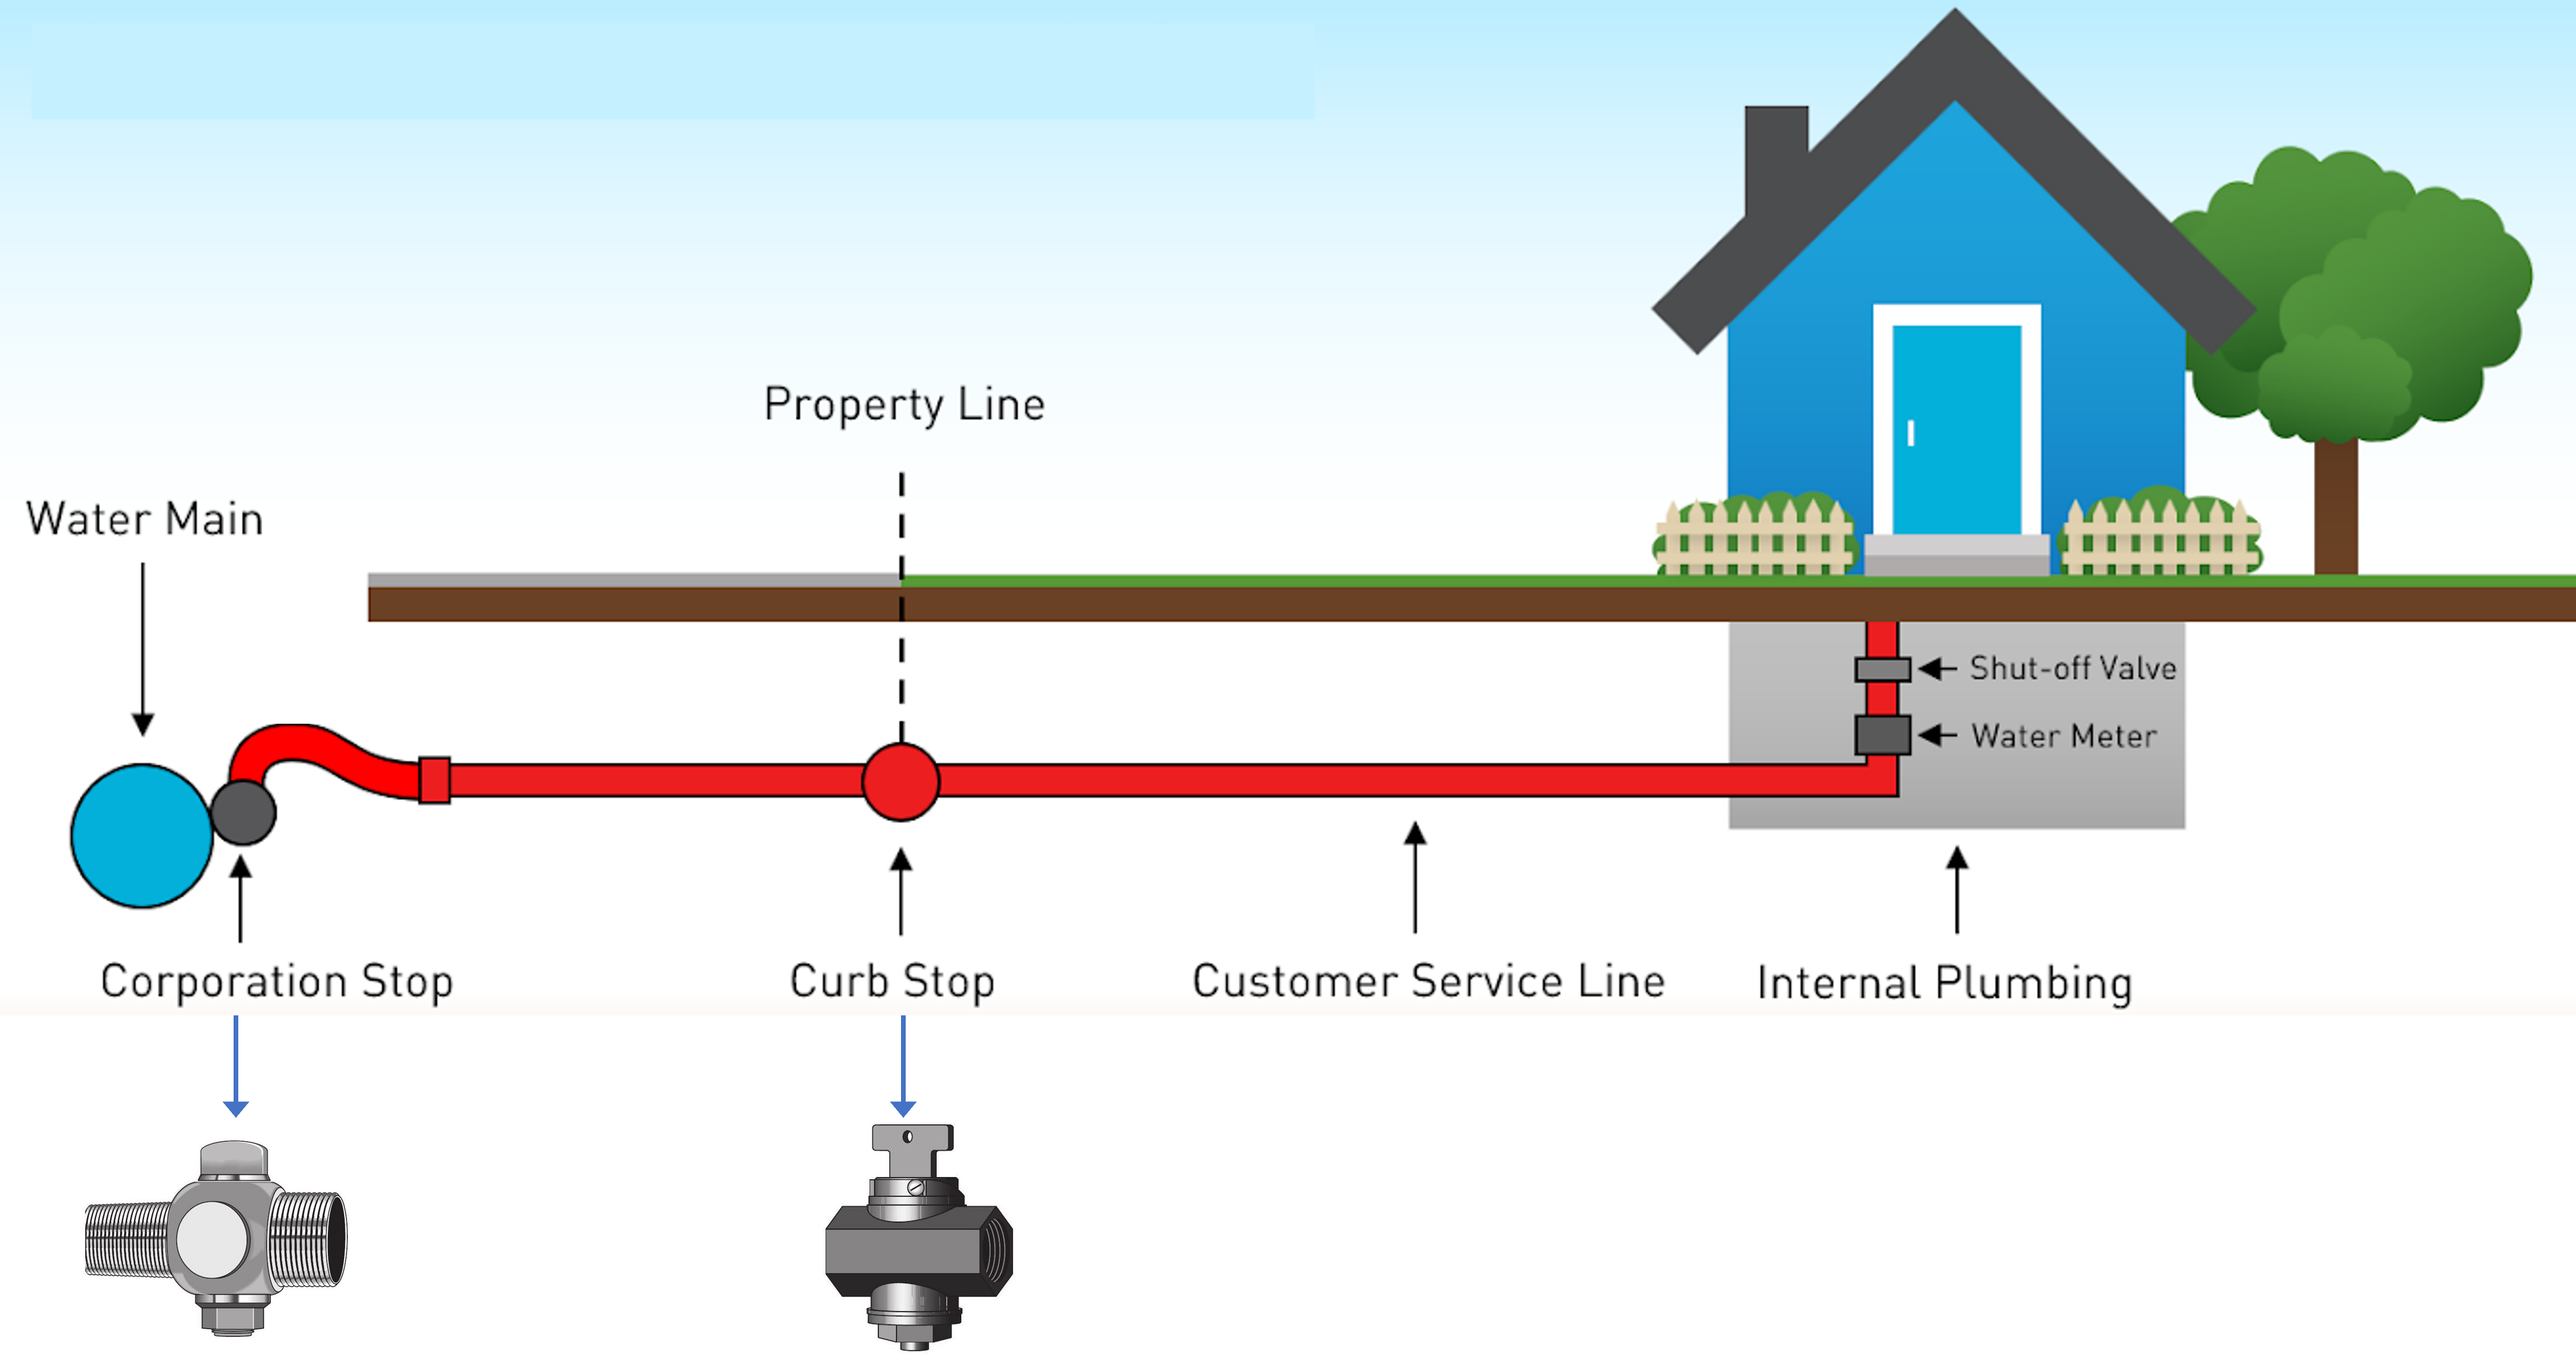
\includegraphics[width=0.85\textwidth]{ServiceLateral}
        \caption{Typical service lateral installation}
\end{center}
\end{figure}


\subsection{Distribution Network Configuration} \index{Distribution network}
\begin{itemize}
\item Distribution network is a system of pipes providing the appropriate quality and quantity of water to a community. 
\item The network construction and layout have to be carefully prepared in order to guarantee enough pressure and ensure hygienically safe water. 
\item Once constructed, maintenance – including repair, leakage control, preventing recontamination, etc. and the operation of pumping stations were gravity pressure is not enough – has to be ensured.
\end{itemize}

The main distribution system network design include:\\
\vspace{1cm}
    \textbf{Dead-end or Tree Distribution System}\index{Distribution network!Dead-end or tree type}\\

    \begin{figure}[H]
        \begin{center}
     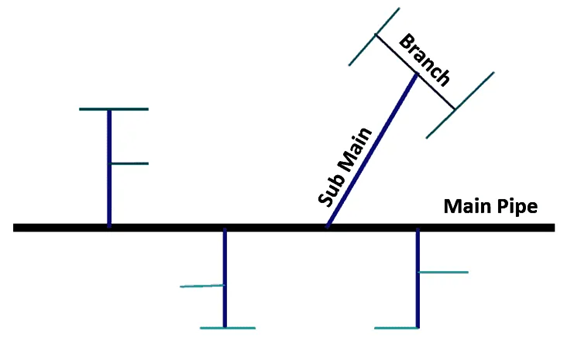
\includegraphics[scale=0.47]{DeadEndTreeDistributionSystem}\\
    \end{center}    
    \end{figure}
\begin{itemize}
\item In this type of water distribution system, one main pipeline runs through the center of the community or building, and the sub-mains branch lines off from both sides. The sub-main lines are  divided into several branch lines for service connection to a particular house.\\
\item Advantages:
      \begin{itemize}[leftmargin=*]
        \item Pipe laying is simple and easy.
        \item Fewer cut-off valves are required - lower O\&M costs.
        \item Maintenance done without disrupting flow
      \end{itemize}
\item Disadvantages:
		\begin{itemize}
		        \item Does not maintain satisfactory pressure in high-rise buildings.
        \item As one pipe provides the water to the entire community or building which is quite risky.
        \item High head loss, requires larger diameter piping
        \item System discharge capacity is limited.
        \item A large number of scour valves are required at the dead ends, which need to be opened periodically for the removal of stale water and sediment
        \item Dead-ends can cause water quality problems and require frequent flushing.
		\end{itemize}
		\end{itemize}
		\newpage
\textbf{Ring Distribution System} \index{Distribution network!Ring type}\\
    \begin{figure}[h!]
        \begin{center}
     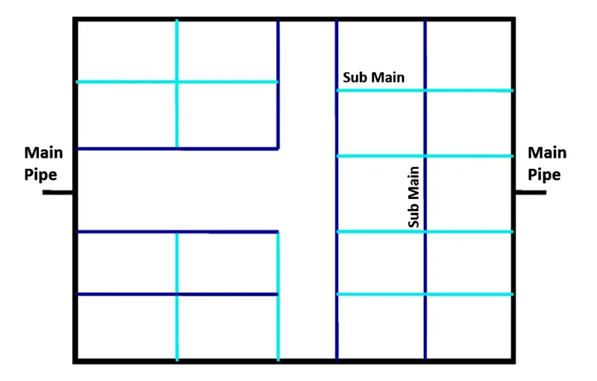
\includegraphics[scale=0.5]{RingDistributionSystem}\\
    \end{center}    
    \end{figure}
\begin{itemize}
\item In this network, the supply main forms a ring around the distribution area.
\item The branches are connected cross-wise to the mains and also to each other.
\item This system is most reliable for a town with well-planned streets and roads.
\item Advantages:\\
\begin{itemize}
        \item Discharge rate is high, low head losses.
        \item Maintenance can be done without disrupting flow.
        \item No endpoints, minimal stagnation.
\end{itemize}
\item Disadvantages:
\begin{itemize}
        \item The length of pipe laying is more which ultimately leads to higher cost.
        \item Several valves are required to control the flow and discharge of water.
\end{itemize}
\end{itemize}
\vspace{1cm}
\textbf{Grid Iron Distribution System}\index{Distribution network!Grid iron type}\\
    \begin{figure}[h!]
        \begin{center}
     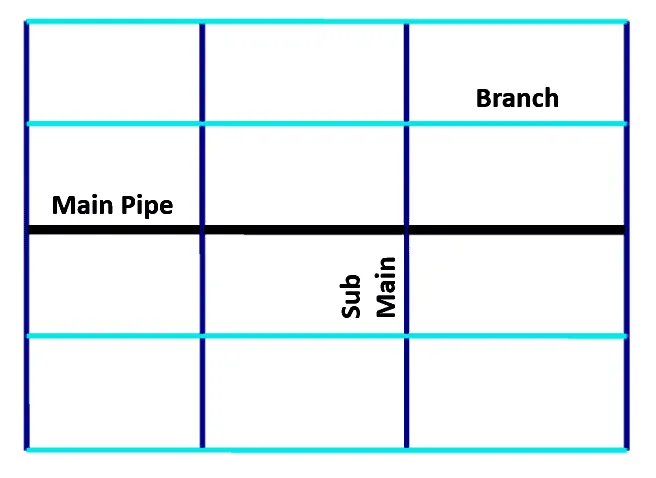
\includegraphics[scale=0.4]{GridIronDistributionSystem}\\
     \end{center}
     \end{figure}
\begin{itemize}
\item Main supply lines run through the center, and sub mains branch off in perpendicular directions. 
\item The branch interconnects the sub-mains. All types of pipes are interconnected - no dead ends.
\item Water can reach any given point from many directions, which allows more flexible operation, particularly for repairs.
\item  It is the most widely used configuration in large municipalities. 
\item Advantages:\\
      \begin{itemize}
        \item Minimal stagnation or sediment deposit.
        \item Water is available at every point with minimum loss of head.
        \item Water is delivered with adequate pressure for firefighting.
        \item During repair, few houses are affected.
      \end{itemize}
\item Disadvantages:\\
       \begin{itemize}
        \item In this system, more cut-off valves are required.
        \item This system requires longer pipe lengths with larger diameters.
        \item The analysis of discharge, pressure, and velocity in the pipes is difficult and cumbersome.
      \end{itemize}
      \end{itemize}

\section{Pipeline Protection} \index{Pipelines! Protection}
Following measures are taken to ensure water distribution pipes are properly installed and protected to reduce risks to prevent contamination of the pipeline contents, protect public health and minimize disruption and costs associated with pipeline failures. 

\subsection{Piping Material Selection}\index{Pipelines! Piping material}
\begin{itemize}
\item The attributes for good pipe materials include:
\begin{itemize}
\item It should have adequate structural strength.

\item Impervious, corrosion-resistant, durable and long, lasting.

\item Cost-effective.

\item Resistance to abrasion.

\item Light weight so that easy to transport and handle.

\item Easy to join, flexible in design, easy to repair and maintain.

\item Environmentally friendly.
\item Ease of locating piping without excavation - pipes with electrical conductive material may be detected using electromagnetic metal detectors whereas pipes made from non-conductive material maybe detected by inducing a signal into the pipe from a valve or hydrant that may be picked up by an above-ground sensor.
\end{itemize}
\item Water distribution pipes material of construction include:
\begin{enumerate}
\item \textbf{Cast iron pipes}
\begin{itemize}
\item Cast iron is the iron made in a foundry via casting - a process that involves melting metal and pouring it into a mold.  It is essentially iron with some carbon in it.  
\item Cast iron typically refers to gray cast iron.  
\item Ductile iron is a type of cast iron but is endowed with higher yield and tensile strength and ductility by the presence of elements including silicon, manganese, magnesium, phosphorus, sulfur, and/or copper.
\item Cast iron pipes attributes:
\begin{itemize}
\item Stable and well suited for high water pressure.
\item  Heavy, which makes them unsuitable for inaccessible places due to transportation problems. 
\item Due to their weight they generally come in short lengths increasing costs for layout and jointing. 
\item Although durable, these pipes are brittle and have a short lifetime. They are subject to cracks and bending from exerted environmental and heavy-traffic pressure, and are susceptible to damage in freezing temperatures caused by expanding ice in the water mains.  
\end{itemize}
\item Ductile iron pipe attributes:
\begin{itemize}
\item Ductile iron pipes are stronger, more durable, and less brittle. 
\item These pipes have more flexibility and are resistant to shocks and vibrations. 
\item Handle freezing temperatures better than cast-iron pipes.
\item Since cast and ductile iron pipes are susceptible to corrosion, a coating is applied to the outside and inside is lined with cement mortar to prevent tuberculation.
\end{itemize}
\end{itemize}

\item \textbf{Steel pipes}\index{Pipelines! Piping material!Steel}
\begin{itemize}
\item Steel is an alloy of iron and carbon.
\item Steel pipes are comparatively expensive, but they are the strongest and most durable of all water supply pipes. 
\item Steel pipes by the virtue of its strength and being lighter than cast-iron pipes, it is an ideal material choice where large diameters pipes are required.
\item They can withstand high water pressure, come in convenient (longer) lengths than most other pipes and thus incur lower installation/transportation costs.
\item They can also be easily welded and are flexible to some extent can be laid on curves.
\item These pipes offer excellent resistance to internal pressure and pressure surges but are susceptible to atmospheric temperature changes which can cause the pipes to buckle.
\item Steel pipes are often provided with an internal asphalt coating to protect against corrosion.
\end{itemize}

\item \textbf{Galvanized pipes} \index{Pipelines! Piping material!Galvanized}
\begin{itemize}
\item Galvanized steel is made from steel that has been coated with a layer of zinc to protect it from rust and corrosion, while galvanized iron is made from iron that has been coated with a layer of zinc.  
\item The use of galvanized steel or iron as a conveyor for drinking water is problematic where water flow is slow or static for periods of time because it causes rust from internal corrosion. 
\item These pipes may also give an unpalatable taste and smell to the water conveyed under corrosive conditions
\end{itemize}

\item \textbf{Asbestos cement (AC) or Transite pipes} \index{Pipelines! Piping material!Asbestos cement (AC) or Transite}
\begin{itemize}
\item In the early 1900s, asbestos cement pipe was first developed by reinforcing concrete with asbestos.
\item Asbestos gave the pipes increased strength, so they could operate under higher pressures. 
\item These pipes were affordable, durable and easy to handle.
\item In the early 1980s, the EPA banned use of all asbestos-related products.
\item Although these asbestos-lined pipes were discontinued, existing AC pipes were not replaced. 
\item Currently, AC pipes account for over 600,000 miles of the United States and Canada’s water distribution pipes.
\end{itemize}

\item \textbf{Concrete pipes} \index{Pipelines! Piping material!Concrete}
\begin{itemize}
\item Reinforced Concrete Pipe (RCP) is made from concrete reinforced with steel
\item RCP pipes can be used up to the head of 60 in and for higher head pre-stressed concrete can be used.
\item There are pipes that are most durable with usual life of about 75 years.
\item The pipes can be cast at site work and thus there is the reduction in transport charges.
\item Although the initial cost is high, overall maintenance cost is less.
\item Inside surface of the pipe can be made smooth and there is no danger of rusting.
\item Transportation and repairs are difficult.
  \end{itemize} 


\item \textbf{High density polyethylene (HDPE) pipes} \index{Pipelines! Piping material!HDPE}
\begin{itemize}
\item HDPE pipe is a popular choice for water mains because of its durability and non-corrosive qualities.
\item These pipes are highly flexible and resistant to fatigue — they can handle usual pressure and pressure from recurring surges which is common in any water distribution system.
\item HDPE pipes cope with high impact not only from traffic but also from soil movement, making these pipes suitable for earthquake-prone regions.
\item These pipes are invaluable for water mains due to the strong joints fused together with heat and pressure. The joint is stronger that the actual pipe and prevents zero water loss, an important aspect for any efficient water distribution system.
\item HDPE to have pipe walls that are 2½ times as  thick in order to provide equivalent pipe strength and safety factor. This adds significantly to the resources  consumed and the cost of the pipe and appurtenances.
\end{itemize}

\item \textbf{Polyvinyl chloride (PVC) pipes} \index{Pipelines! Piping material!PVC}
\begin{itemize}
\item PVC water pipe is made by extrusion of unplasticized polyvinyl chloride. \item PVC pipes used for water mains comply with the AWWA C-900 standard for PVC pipes. This distinguishes it from other PVC water pipe that has a thinner wall.
\item The material is lightweight and easy to install. 
\item One disadvantage to PVC pipe is installation in contaminated soils, where fuel oils, gasoline, and other organic compounds may permeate the pipe wall.
\end{itemize}
\end{enumerate}
\end{itemize}

\subsection{Pipeline Joints and Couplings}  \index{Pipelines!Joints}
\begin{itemize}
\item Joints and couplings join individual pipes and to other appurtenances including valves, hydrants etc. together, creating a continuous flow path in the piping systems. 
\item These are designed to provide secure and leak-free connections, ensuring the efficient transfer of fluids or gases and pipe material specific.
\item Typically used joints and couplings:
\begin{enumerate}
\item Mechanical joint (MJ) \index{Pipelines!Joints!Mechanical joint}\\
\begin{minipage}{0.3\textwidth}
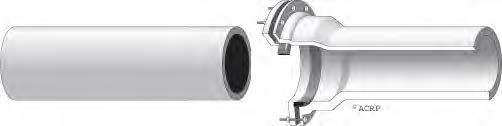
\includegraphics[width=1\linewidth]{MechanicalJoint2}
\end{minipage}
\begin{minipage}{0.1\textwidth}
\end{minipage}
\begin{minipage}{0.55\textwidth}
\begin{itemize}
\item Originally developed for use with cast iron and ductile iron water mains.
\item Primarily used for connecting pipes, valves and hydrants.
\item MJ is combined with thrust blocks for a fully restrained installation.
\item Mechanical joint restraints use a flange/gland) with set screws and lug-style clamping devices and a gasket to make a watertight seal.
\end{itemize}
\end{minipage}
\vspace{0.3cm}
\item Rubber ring push-on joint \index{Pipelines!Joints!Rubber ring push-on}\\
\begin{minipage}{0.3\textwidth}
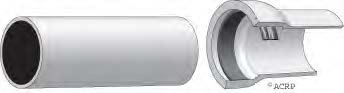
\includegraphics[width=1\linewidth]{RubberRingPushonJoint}
\end{minipage}
\begin{minipage}{0.1\textwidth}
\end{minipage}
\begin{minipage}{0.55\textwidth}
\begin{itemize}
\item Push-on joints are comprised of a special bell with an internal groove, a plain end, and rubber gasket which is seated into the bell's groove.
\item This joint forms a watertight seal.
\item Used with ductile iron pipe installation.
\end{itemize}
\end{minipage}
\vspace{0.3cm}
\item Dresser coupling \index{Pipelines!Joints!Dresser coupling}\\
\begin{minipage}{0.3\textwidth}
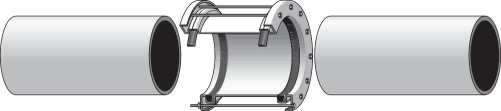
\includegraphics[width=1\linewidth]{DresserCoupling1}
\end{minipage}
\begin{minipage}{0.1\textwidth}
\end{minipage}
\begin{minipage}{0.55\textwidth}
\begin{itemize}
\item Dresser coupling joint is a type of mechanical coupling.
\item It is used to join two plain ends of pipes.
\item It consists of a cylindrical sleeve with two serrated ends, which grips the spigot (male end) and socket (female end) of two pipes.
\item Dresser couplings are suitable for joining steel, cast and ductile iron, PVC and HDPE pipes.
\item Dresser couplings create flexible, non-rigid pipeline joints accepting
expansion, contraction, vibration and line deflection.
\end{itemize}
\end{minipage}
\vspace{0.3cm}
\item Bell and spigot joint \index{Pipelines!Joints!Bell and spigot joint}\\
\begin{minipage}{0.3\textwidth}
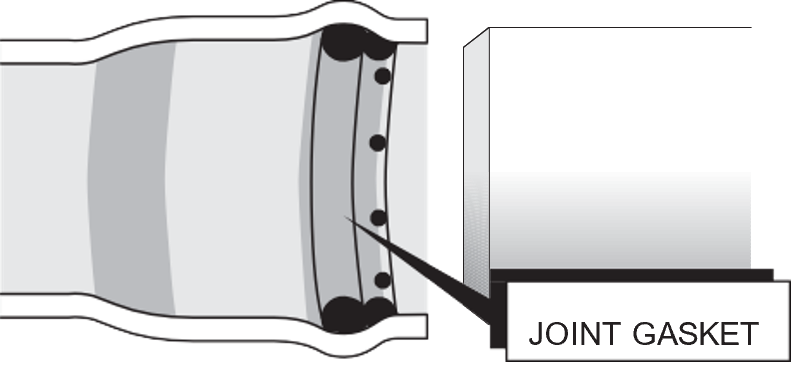
\includegraphics[width=0.7\linewidth]{BellandSpigotJoint1}
\end{minipage}
\begin{minipage}{0.1\textwidth}
\end{minipage}
\begin{minipage}{0.55\textwidth}
\begin{itemize}
\item A form of joint used on pipes that have an enlarged diameter or bell at one end and a spigot at the other that fits into and is laid in the bell.
\item Used for joining ductile iron and copper pipes.
\end{itemize}
\end{minipage}
\vspace{0.3cm}
\item Flange joint \index{Pipelines!Joints!Flange joint}\\
\begin{minipage}{0.3\textwidth}
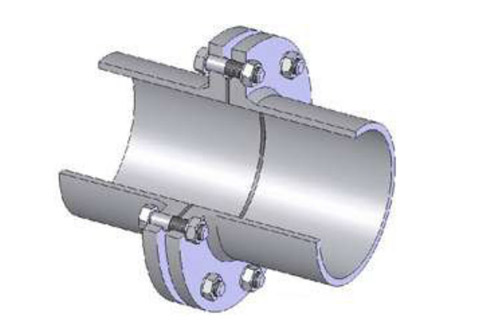
\includegraphics[width=0.8\linewidth]{FlangeJoint1}
\end{minipage}
\begin{minipage}{0.1\textwidth}
\end{minipage}
\begin{minipage}{0.55\textwidth}
\begin{itemize}
\item Flanged pipe is generally specified for above ground service where rigid, restrained joints are needed.
\item The main use of flange is to connect pumps, pipes, valves, and other equipment.
\end{itemize}
\end{minipage}
\vspace{0.3cm}
\item Victaulic coupling \index{Pipelines!Joints!Victaulic coupling}\\
\begin{minipage}{0.3\textwidth}
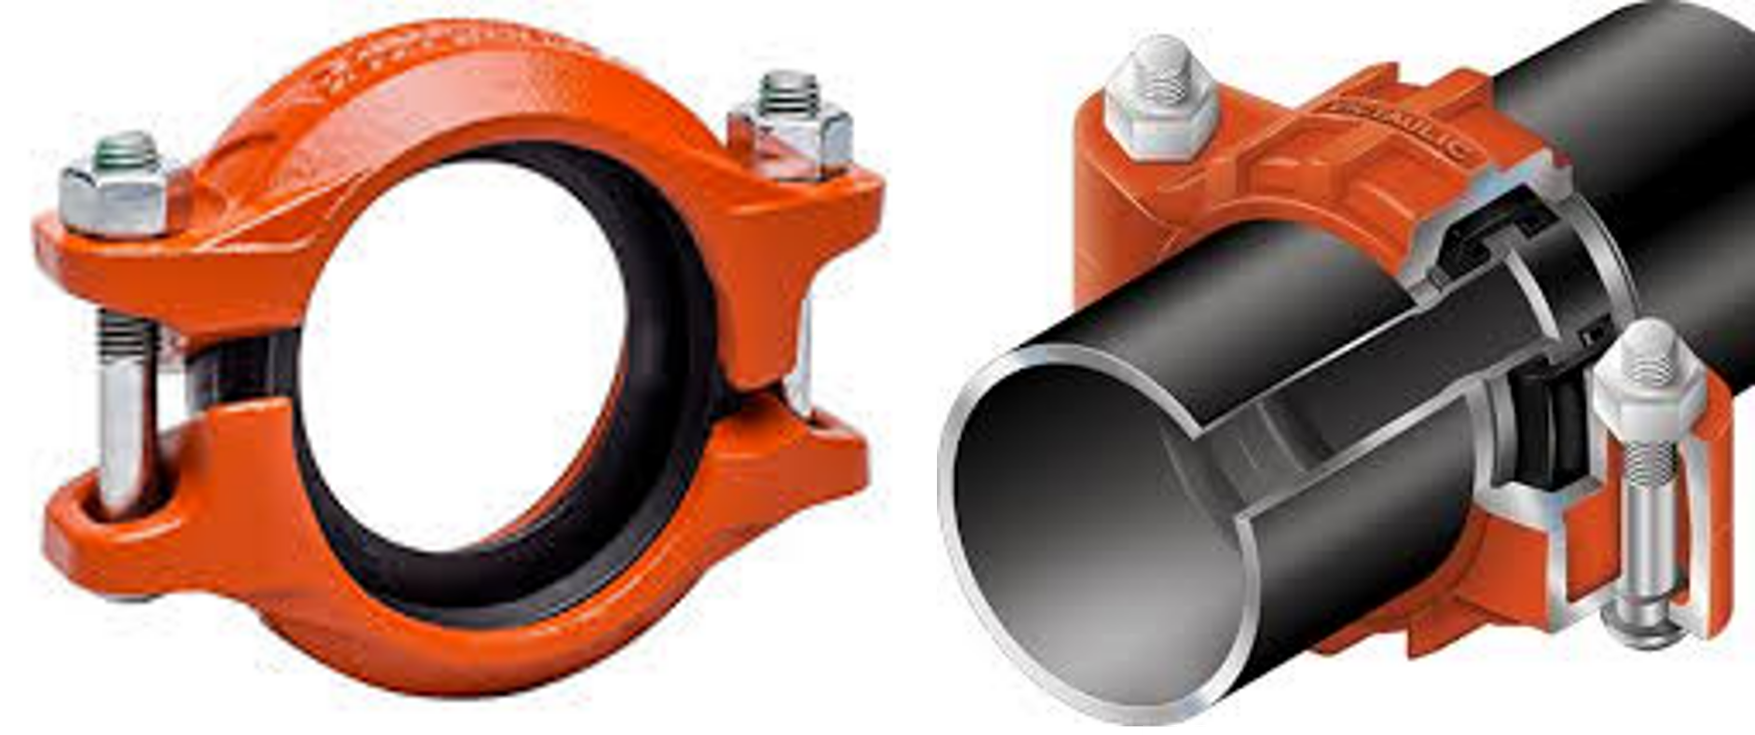
\includegraphics[width=1\linewidth]{Victaulic}
\end{minipage}
\begin{minipage}{0.1\textwidth}
\end{minipage}
\begin{minipage}{0.55\textwidth}
\begin{itemize}
\item In the Victaulic coupling a groove is formed near the ends of the two pipes that are to be joined. A flexible (often rubber) gasket is placed around both pipe ends, connecting them. The metal housing – a sleeve of sorts – is then placed over the gasket and joined pipes and tightened with nuts and bolts.
\item Victaulic couplings now exist that can accommodate most types of piping material, including steel, PVC, HDPE, ductile iron and copper tubing.
\end{itemize}
\end{minipage}
\end{enumerate}
\end{itemize}
\vspace{0.3cm}
\subsection{Basic Water Main Installation} \index{Water main installation}
\begin{enumerate}
\item Trenching and trench preparation
\begin{itemize}
\item To prevent drinking water contamination from adjacent sewage and other water pipes, drinking water pipes must meet standards Meeting standards to ensure California Code of Regulations, Title 22,
Division 4, Chapter 16, Section 64572 establishes criteria for the separation of new water mains from non-potable pipelines. These standards include:
\begin{itemize}
\item New water mains and new supply lines shall not be installed in the same trench as and \textbf{shall be at least 10 feet horizontally from and one foot vertically above, any parallel pipeline} conveying untreated/treated sewage, disinfected secondary recycled water or hazardous fluids such as fuels, industrial wastes, and wastewater sludge.
\item New water mains and new supply lines shall be installed at \textbf{least 4 feet horizontally from, and one foot vertically above, any parallel pipeline conveying tertiary recycled water, and storm drainage.}
\item New water mains \textbf{shall not be installed within 100 horizontal feet of the nearest edge of any sanitary landfill, wastewater disposal pond, or hazardous waste disposal site, or within 25 horizontal feet of the nearest edge of any cesspool, septic tank, sewage leach field, seepage pit, underground hazardous material storage tank, or groundwater recharge project site.}
\end{itemize}
\item Water main installation begins with excavation which is expensive and dangerous.  Before excavation can begin, the project must be well planned and all safety elements must be considered.
\item All trenching and excavations related safety hazards needs to be mitigated and applicable  To protect the trench and workers from traffic.
\item After the trench is prepared, inspect the pipe for defects, damage, oil, dirt, grease, and/or foreign matter.
\item Any unsound material should be replaced and all foreign matter or dirt should be removed from the interior of the pipe before lowering into the trench.
\item Before lowering the pipe into the trench the trench bottom should be smooth and free of material like large stones or large dirt clods.
\end{itemize}
\item Pipe installation
\begin{itemize}
\item Lower the pipes, and other necessary equipment carefully into the trench.
\item Before connecting the pipe:
\begin{itemize}
  \item Inspect the pipe ends to be sure that no dirt or foreign material is on the joint locations.
  \item Clean the pipe end around the entire circumference from the end spigot to 1 inch above the reference line.
  \item Once the pipe is cleaned, be careful during installation to ensure gravel does not enter into the line.
\item Bedding is a granular material placed in the bottom of a pipe trench to support the pipe. 
\item Types of bedding include pea gravel, sand, and select native soil material.
\item A lack of proper uniform support can lead to “beam” breakage \index{Beam breakage} of the pipe.
\end{itemize}
\item To prevent pipe joints from uncoupling due to thrust forces created in a pipeline where it changes direction, and other damage from internal pressure or water hammer, thrust blocks are used.
\item Thrust blocks are often made of concrete and steel reinforcement rods cast in place or large precast concrete blocks. 
\item It is important that thrust blocks rest against undisturbed soil with sufficient bearing area. 
\item There are standard engineering formulas to determine the thrust exerted within a pipeline and the size of thrust block necessary for a given type of soil.
    \begin{figure}[H]
        \begin{center}
     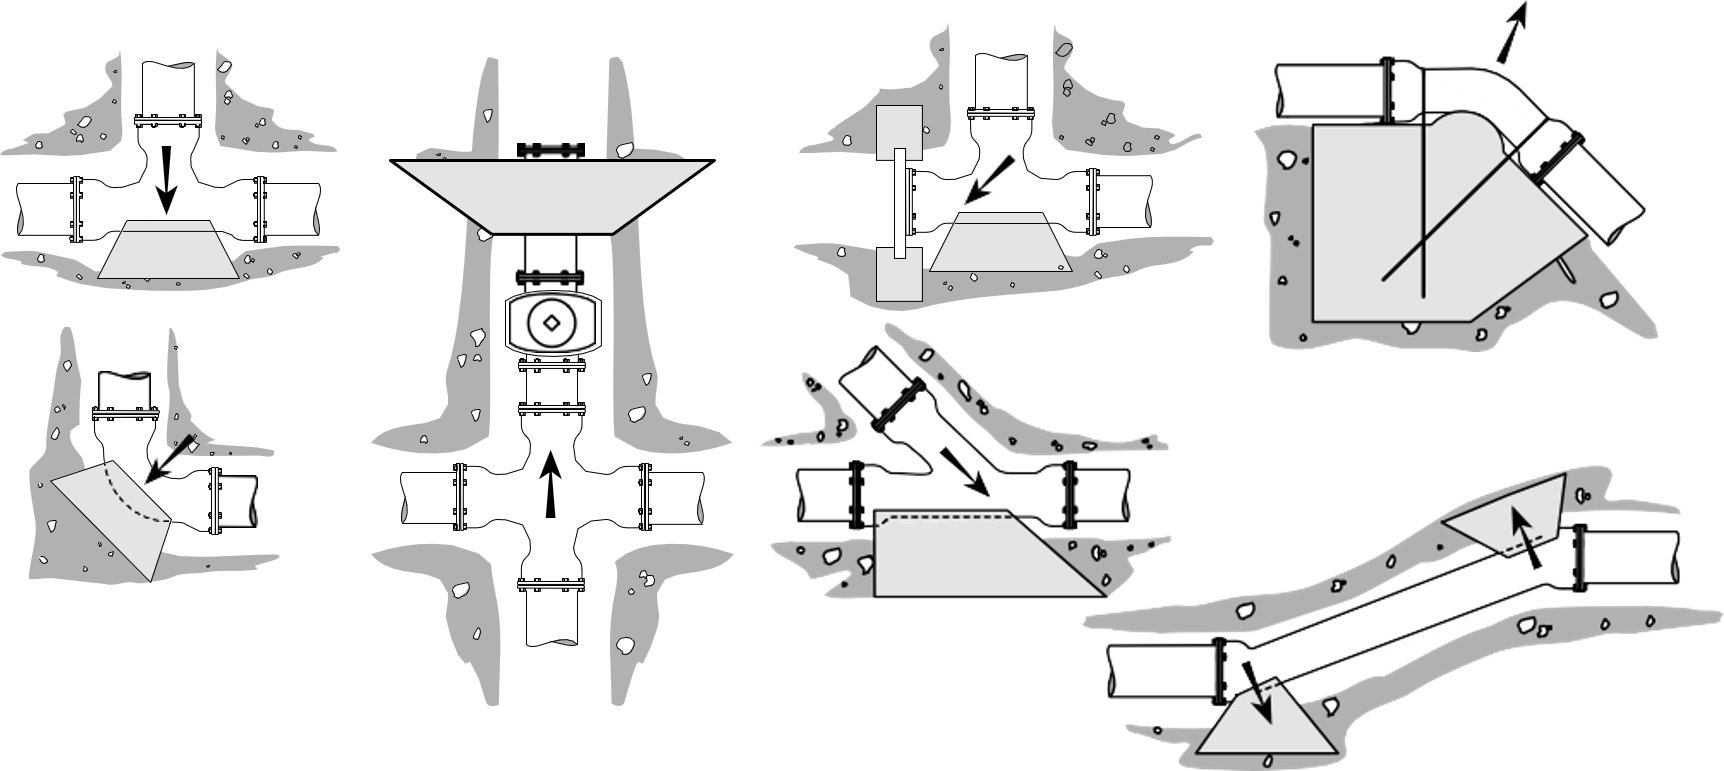
\includegraphics[scale=1]{ThrustBlocks1}
     \caption{Thrust blocks} \index{Thrust blocks}
    \end{center}    
    \end{figure}
\item After the water main pipe and fittings have been installed in the trench, the excavation must be backfilled with suitable material.
\item Only clean sand or selected soil should be used for the first layer. The bedding around the pipe should be of uniform size and material. Allowing materials of various sizes such as large rocks could cause the pipe to fracture during settlement.
\item The first layer of backfill should be placed equally on both sides of the pipe, up to about the center of the pipe. This material should then be compacted, a process often called haunching.
\item Depending on the area and conditions, generally another layer of backfill is placed over the pipe and again compacted to protect and secure the pipe.
\item The trench needs refilled appropriately. The backfill material should be compacted at 12 inch intervals to minimize settlement.
\item Backfill practices vary depending on type of pipe, local soil conditions and regulatory requirements. Proper backfilling is very important:
\item Improper compaction could result in a lack of proper uniform pipe support which may lead to “beam” breakage of the pipe. 
\item Large backfill material will increase probability of main break
\item After the trench has been backfilled, the new main must be pressure tested to determine whether there are any leaks.
\item The top of the pipe should be buried not less than 1 foot below the frost line. In those locations where frost is not a factor, the depth of cover should be not less than 2-1/2 feet to prevent mechanical damage.
\end{itemize}
\item Pipe disinfection
\begin{itemize}
\item All new sections of water mains must be thoroughly disinfected per AWWA Standard C651-05.
\item Sections of pipes, fittings and valves and other items that will be not disinfected by the filled line must be pre-cleaned and disinfected.
\item To properly disinfect water mains, different methods can be applied. Due to the dangers of chlorine it is advised that the operator choose the best method that suits the facility's needs.
\item The pipe disinfection process involves use of chlorine disinfectant of a specified concentration and time followed by flushing and sampling for bacteriological quality.
\item One or more fire hydrants should be used for flushing so that a velocity of around $5 \mathrm{ft} / \mathrm{s}$ is obtained in the pipe.
\item This velocity should be maintained long enough to allow two or three complete changes of water and for the water to run visibly clean. - Gravel in the line is an indication of improper installation.
\item The highly chlorinated water will probably kill grass, so the flow should be carried to a disposal site through hoses.
\item In some cases, the water may need dechlorinated before it is released to a waterway.

\end{itemize}

\end{enumerate}

\section{Water storage}\index{Water storage}
\begin{itemize}
\item Water  storage reservoir in a water distribution system allows for:
\begin{enumerate}
\item Maintaining water supply pressure - typically maintained by the water level in the storage reservoir.
\item As water demand changes during the day, the water reservoir provides the buffer capacity to meet the demand during peak period.  Allows for leveling out the pumping demands by allowing the pumping system to fill the reservoir to a specific level after which the pumps are shut off, and water is drawn from the reservoir until the level drops to a predetermined point at which time the pumps restart.
\item Providing fire fighting demand which may account for as much as fifty percent of total storage. In addition, fire-fighting demands must be met during main line breaks, power outages, and maximum customer demands.
\item Providing a point to blend different water supplies.
\item Providing ability to supply water during power outages and during maintenance of transmission mains.
\item Providing the detention time for chlorine disinfection to meet the water quality requirements.
\end{enumerate}
\item There are four basic type of storage reservoirs: \index{Water storage!Types of reservoirs}
\begin{enumerate}
\item Underground reservoir
\item Ground level reservoir
\item Elevated reservoirs which include elevated tanks and standpipes
\item Hydropneumatic tanks which are tanks which contain 1/3 air and 2/3 water.  The air in the tank is compressed as the tank fills with water and the pressurized air pushes water out of the tank.
\end{enumerate}
\item Typical material of construction include welded and bolted steel and cast-in-place and pre-stressed concrete.  Some smaller tanks such as the hydropneumatic tank is made from fiberglass.
\item Newly-installed distribution reservoir or distribution reservoir that has been taken out of service for repair or inspection is required to be disinfected and sampled for bacteriological quality in accordance with the American Water Works Association Standard C652-02 \index{Disinfection!AWWA Standard!C652-02 Disinfection of distribution reservoir}. If the results of the bacteriological sampling are positive for coliform bacteria, the reservoir shall be re-sampled for bacteriological quality and the test results shall be submitted to the State Board for review and approval before the reservoir is placed into service.
\begin{figure}[h]
\begin{center}
        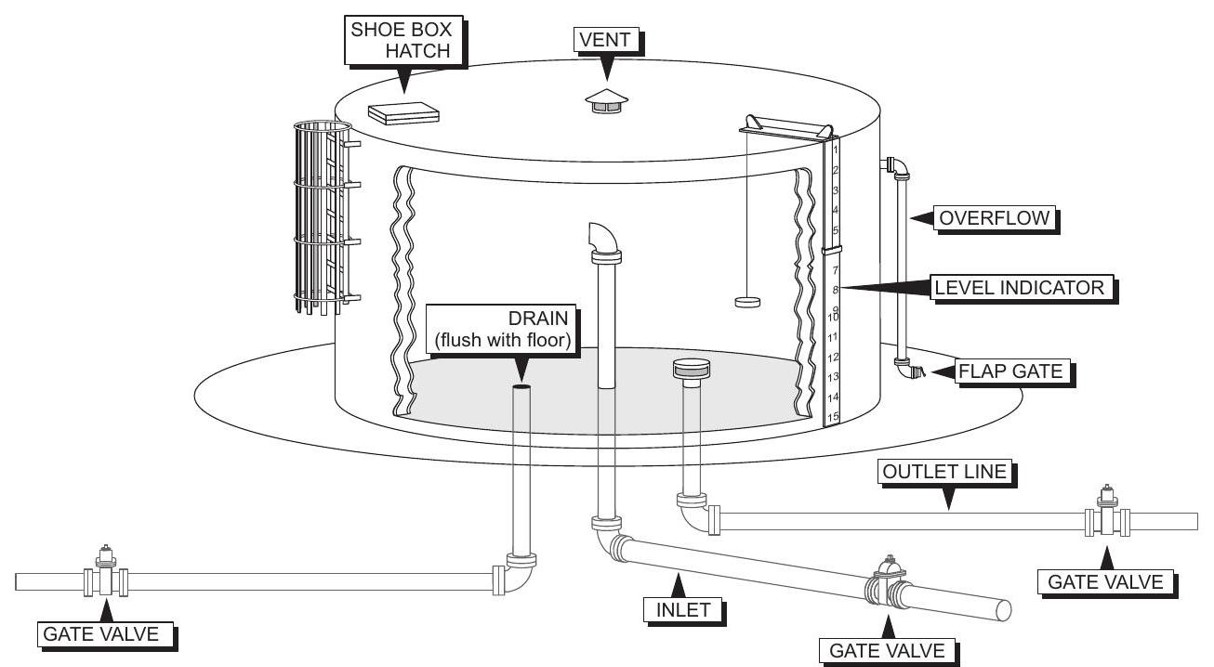
\includegraphics[scale=0.3]{ReservoirPiping}
        \caption{Typical reservoir piping}
\end{center}
\end{figure}
\end{itemize}
   \vspace{-2em} 
\section{Valves Used in Water Distribution}\index{Valves used in water distribution}
\begin{itemize}
\item  Valves are a critical component of every water systems.
\item Main type of valves used in the water distribution system include:
\begin{enumerate}
\item Flow control and isolation valves
\item Air valves
\item Backflow prevention valves
\end{enumerate}
\item Valves can be classified based upon the movement of the closure element as:
\begin{enumerate}
\item Rotary valve:
\begin{itemize}
\item The stem modes from fully open to fully closed position by rotating 90 degrees. 
\item Rotary valves include:  plug, ball and butterfly valves.
\end{itemize}
\item Linear valves:
\begin{itemize}
\item Also known as multi-turn valves, these have a sliding-stem design that pushes a closure element into an open or closed position.
\item Linear valves include:  globe, gate and check valves.
\item They offer flow control capabilities.
\end{itemize}
\end{enumerate}
\item Valves are used for the following applications:
\begin{itemize}
\item Flow and pressure regulation
\item System isolation
\item Air relief
\item Backflow or cross-connection prevention
\item Pressure reducing and pressure sustaining
\item Controlling levels and preventing overflow in elevated tanks and standpipes - Altitude valves
\item Blowoff and drain valves for removing accumulated sediments from low spots and for dewatering lines and reservoirs.
\item Controlling level of water in tanks and activating controls - Float valves
\end{itemize}
\end{itemize}
%   \vspace{-2em} 
\subsection{Flow Control and Isolation Valves}\index{Valves}
\begin{itemize}
\item These valves are used for controlling flows or for isolation of pipelines.
\item Valve selection is based upon the application elements including size of pipe and water pressure.
\item Tables ~\ref{table:Valve1} and ~\ref{table:Valve2} summarize the properties and use of the commonly used distribution system valves. 
\end{itemize}
\newpage
\thispagestyle{empty}
   \vspace{-2em} 
\begin{landscape}
\begin{table}
  \centering
  \begin{tabular}{| m{7cm} m{10cm} | m{7cm} | }
    \hline
\multicolumn{2}{c}{Globe Valve} & \multicolumn{1}{c}{Use} \\ \hline
    \begin{minipage}{.5\textwidth}
    \begin{center}
    \hspace{0.5cm}
%    \tcbox[colframe=green!30!black,
%           colback=green!30]{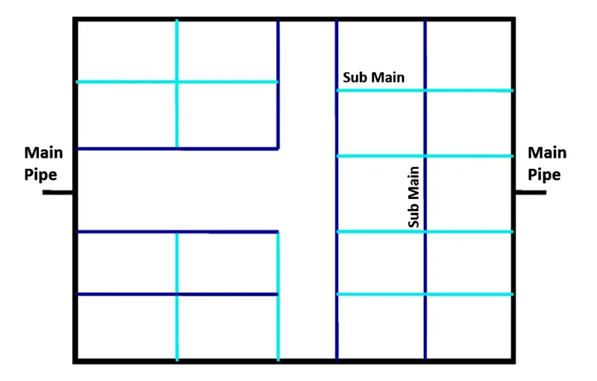
\includegraphics[scale=0.5]{RingDistributionSystem}}    
     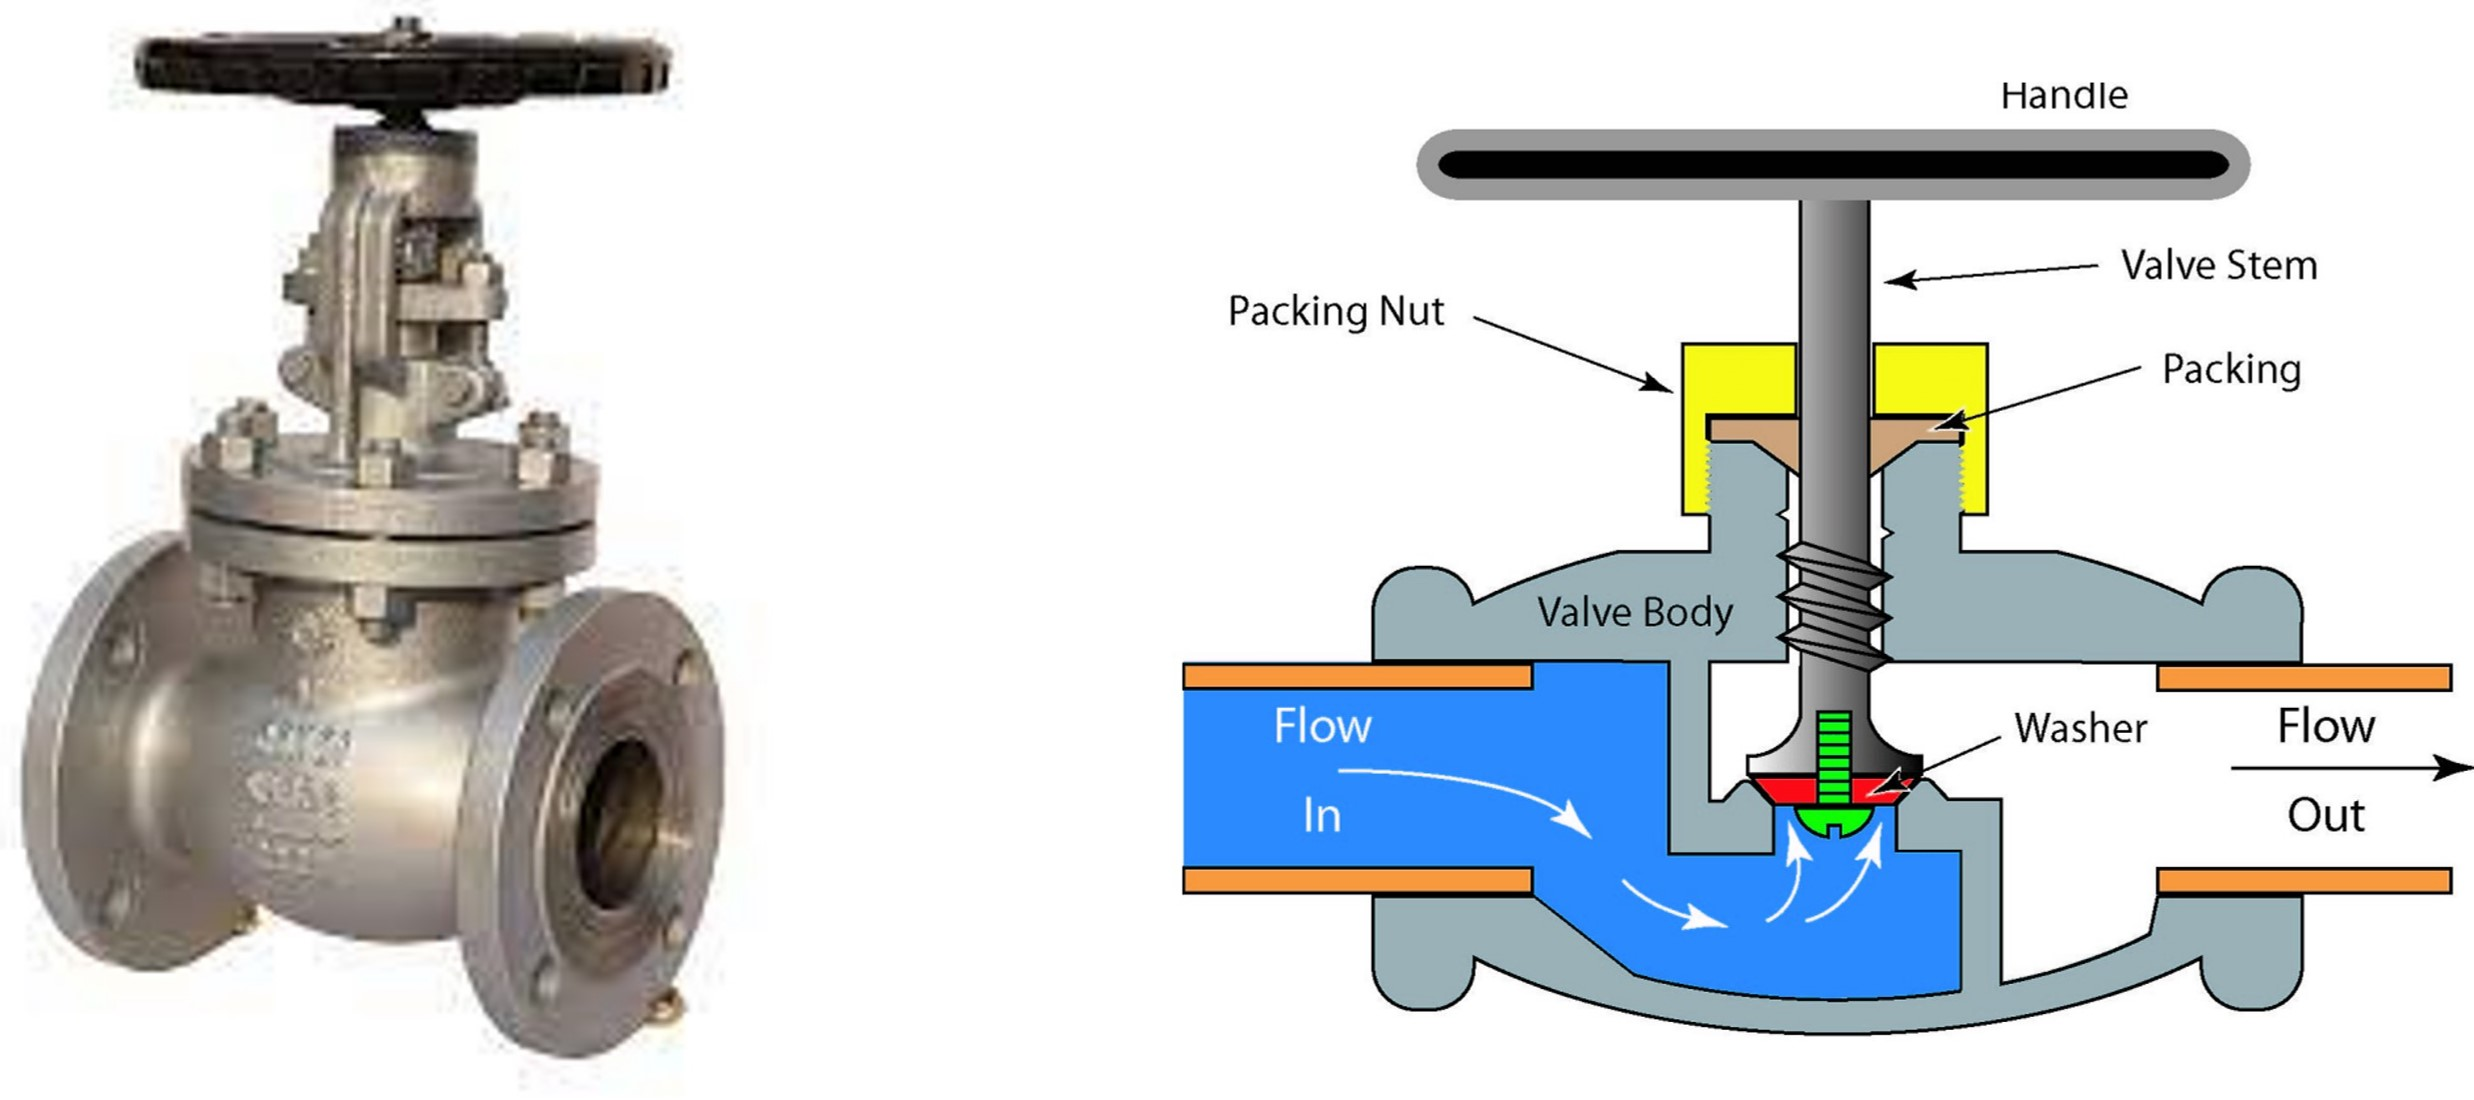
\includegraphics[scale=0.35]{GlobeValve1}\\
     \end{center}
    \end{minipage}
    &
  \scriptsize{\begin{itemize}[topsep=5pt, partopsep=0pt]
  \item Linear stroke type valve \item Has a spherical shape of valve body. \item Globe valves have a movable closure that moves up and down inside of the valve body. \item Valve body is divided into two halves by a partition or baffle.  \item A small horizontal disc or plug is the closure member which can move up and down attached to the stem, thus opening or closing the valve. \item The discs in contact with the seat closes the valve. The seat can be damaged by formation of solid deposits. Hence globe valves are suitable only for clean service.
  \end{itemize}}  
    &
    %\begin{minipage}[t]{5cm}
        \vspace{0.4cm}
      \begin{itemize}[leftmargin=*]
      \scriptsize{
       \item Globe valves have higher pressure drops in comparison to other valves.
        \item \textbf{Used for flow and pressure control in large size applications and for isolation in small sizes.  }
        \item The torturous path of the flow through a globe valve causes a larger pressure drop compared to other valves. 
        \item An \textbf{altitude valve} is a type of a globe valve, is used for controlling the level of water in a reservoir.  It opens and closes to fill a high-level tower or tank hydraulically and it functions by sensing the static level of water in the tower.}
      \end{itemize}
    %\end{minipage}
  
    \\ \hline

\multicolumn{2}{c}{Plug Valve} & \multicolumn{1}{c}{Use} \\ \hline
    \begin{minipage}{.3\textwidth}
%    \tcbox[colframe=green!30!black,
%           colback=green!30]{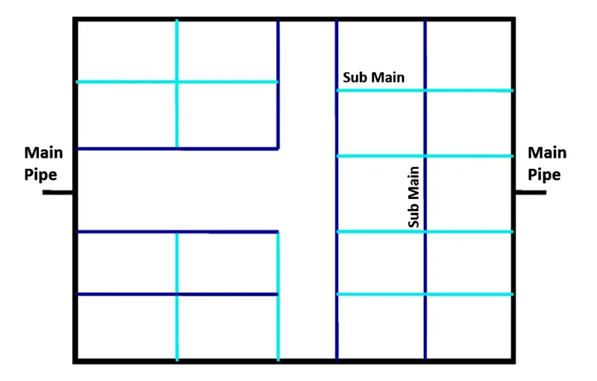
\includegraphics[scale=0.5]{RingDistributionSystem}}    
   \vspace{-2em} 
     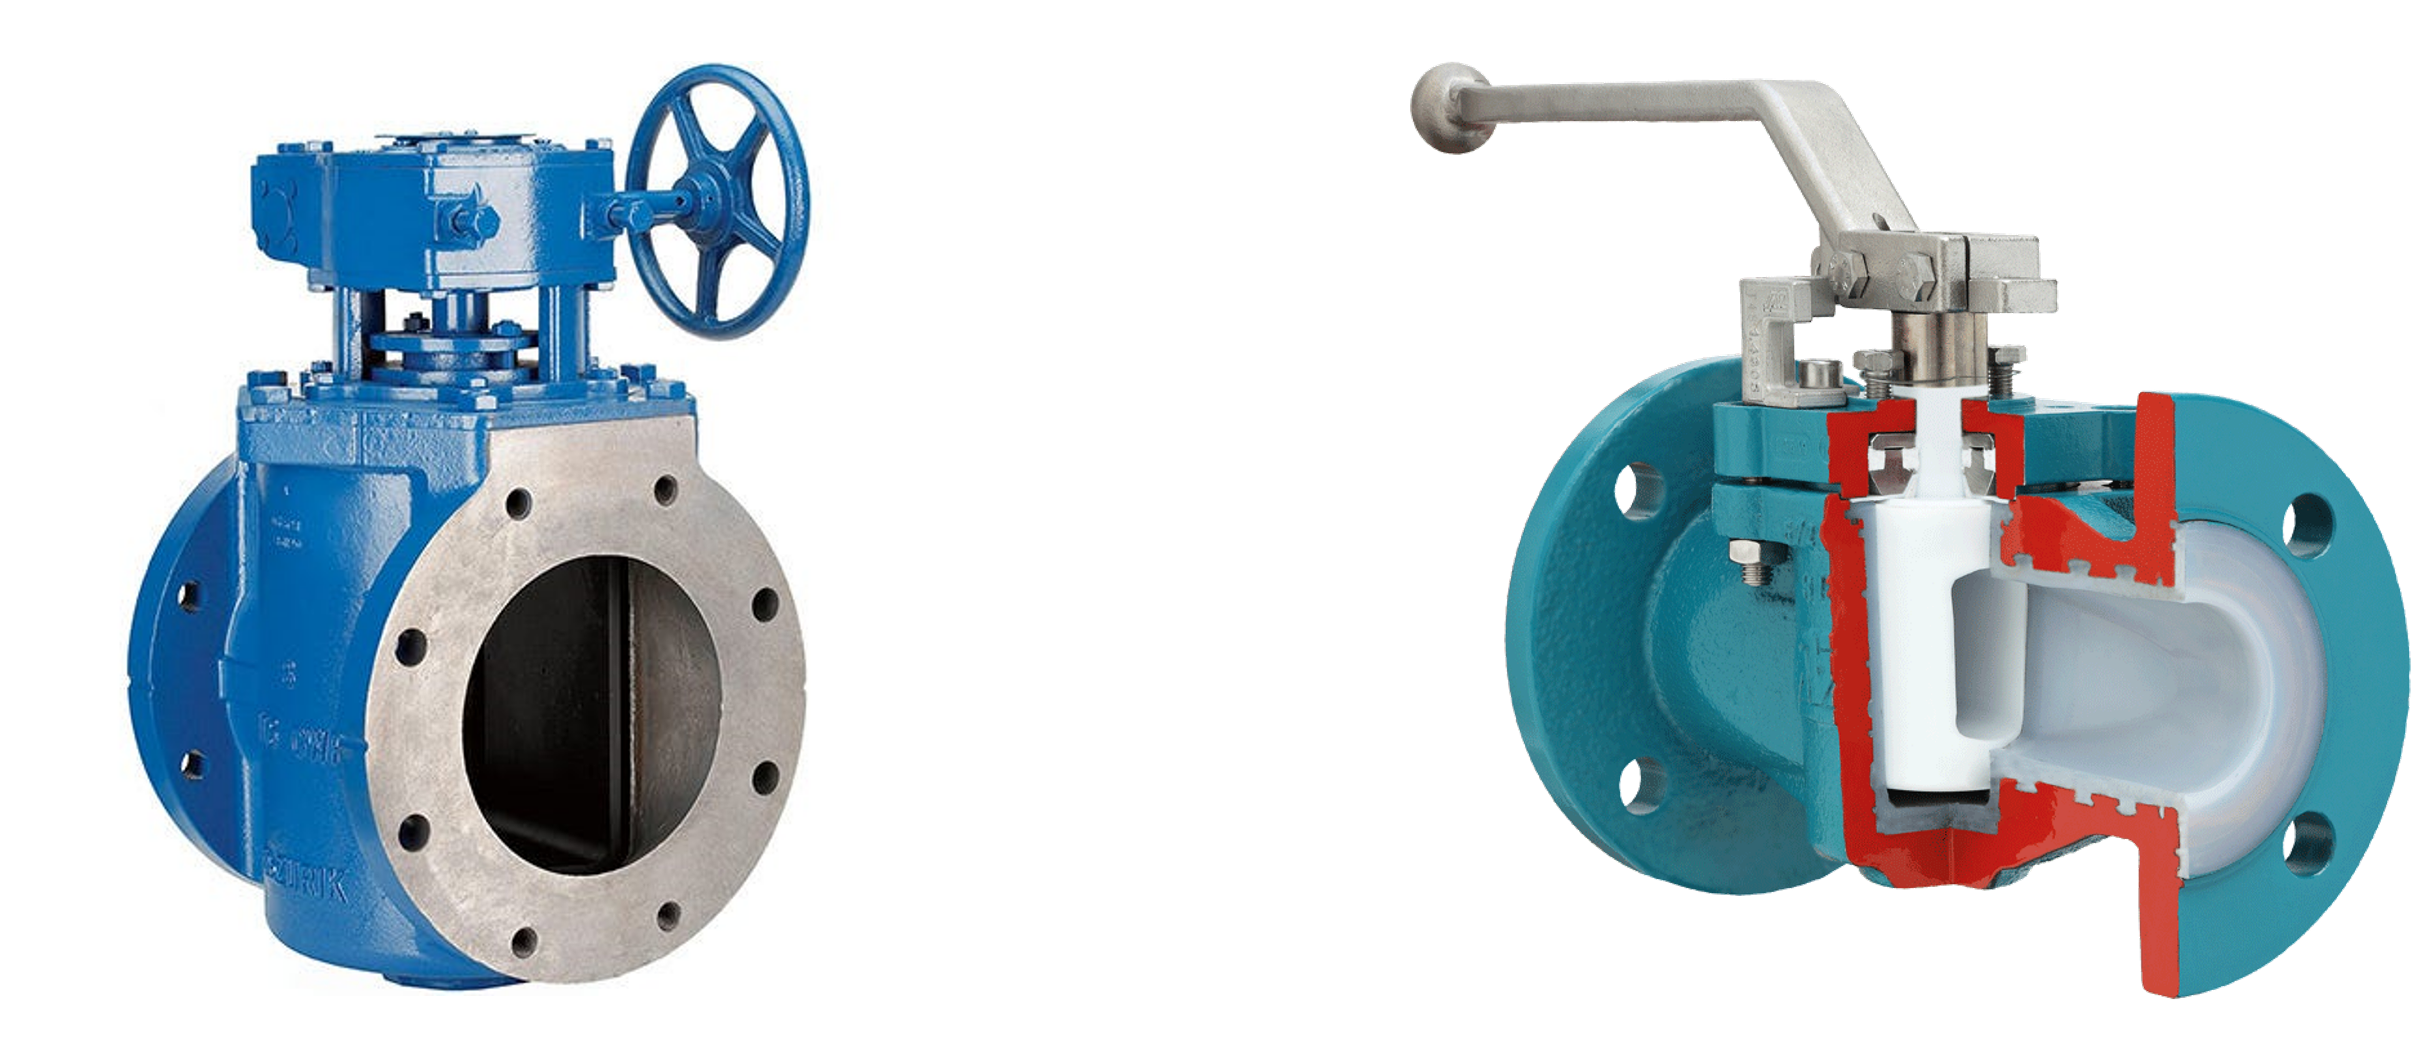
\includegraphics[scale=0.4]{PlugValve1.png}\\
    \end{minipage}
    &
  \scriptsize{\begin{itemize}[topsep=5pt, partopsep=0pt]
  \item Rotary stroke type valve \item Valves have a cylindrical or conically tapered "plugs" which can be rotated inside the valve body to control flow through the valve. \item The plugs in plug valves have one or more hollow passageways going sideways through the plug, so that fluid can flow through the plug when the valve is open.
  \end{itemize}}  
    &
    %\begin{minipage}[t]{5cm}
        \vspace{0.4cm}
      \begin{itemize}[leftmargin=*]
      \scriptsize{
        \item The plug valve is the simplest of all valves. \item The movable closure has a hole through which water is permitted to pass. \item $\mathrm{A} 1 / 4$ turn turns the valve from open to closed. \item \textbf{Commonly used as the isolation valves on the customer service lines Corporation Stops.} }
      \end{itemize}
    %\end{minipage}
  
    \\ \hline
\multicolumn{2}{c}{Gate Valve} & \multicolumn{1}{c}{Use}\\ \hline
    \begin{minipage}{.3\textwidth}
%    \tcbox[colframe=green!30!black,
%           colback=green!30]{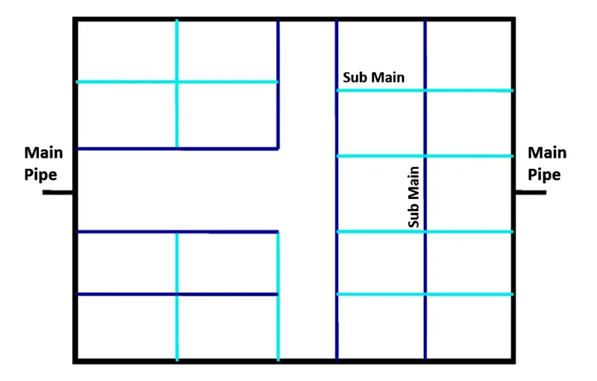
\includegraphics[scale=0.5]{RingDistributionSystem}}    
   \vspace{-2em} 
     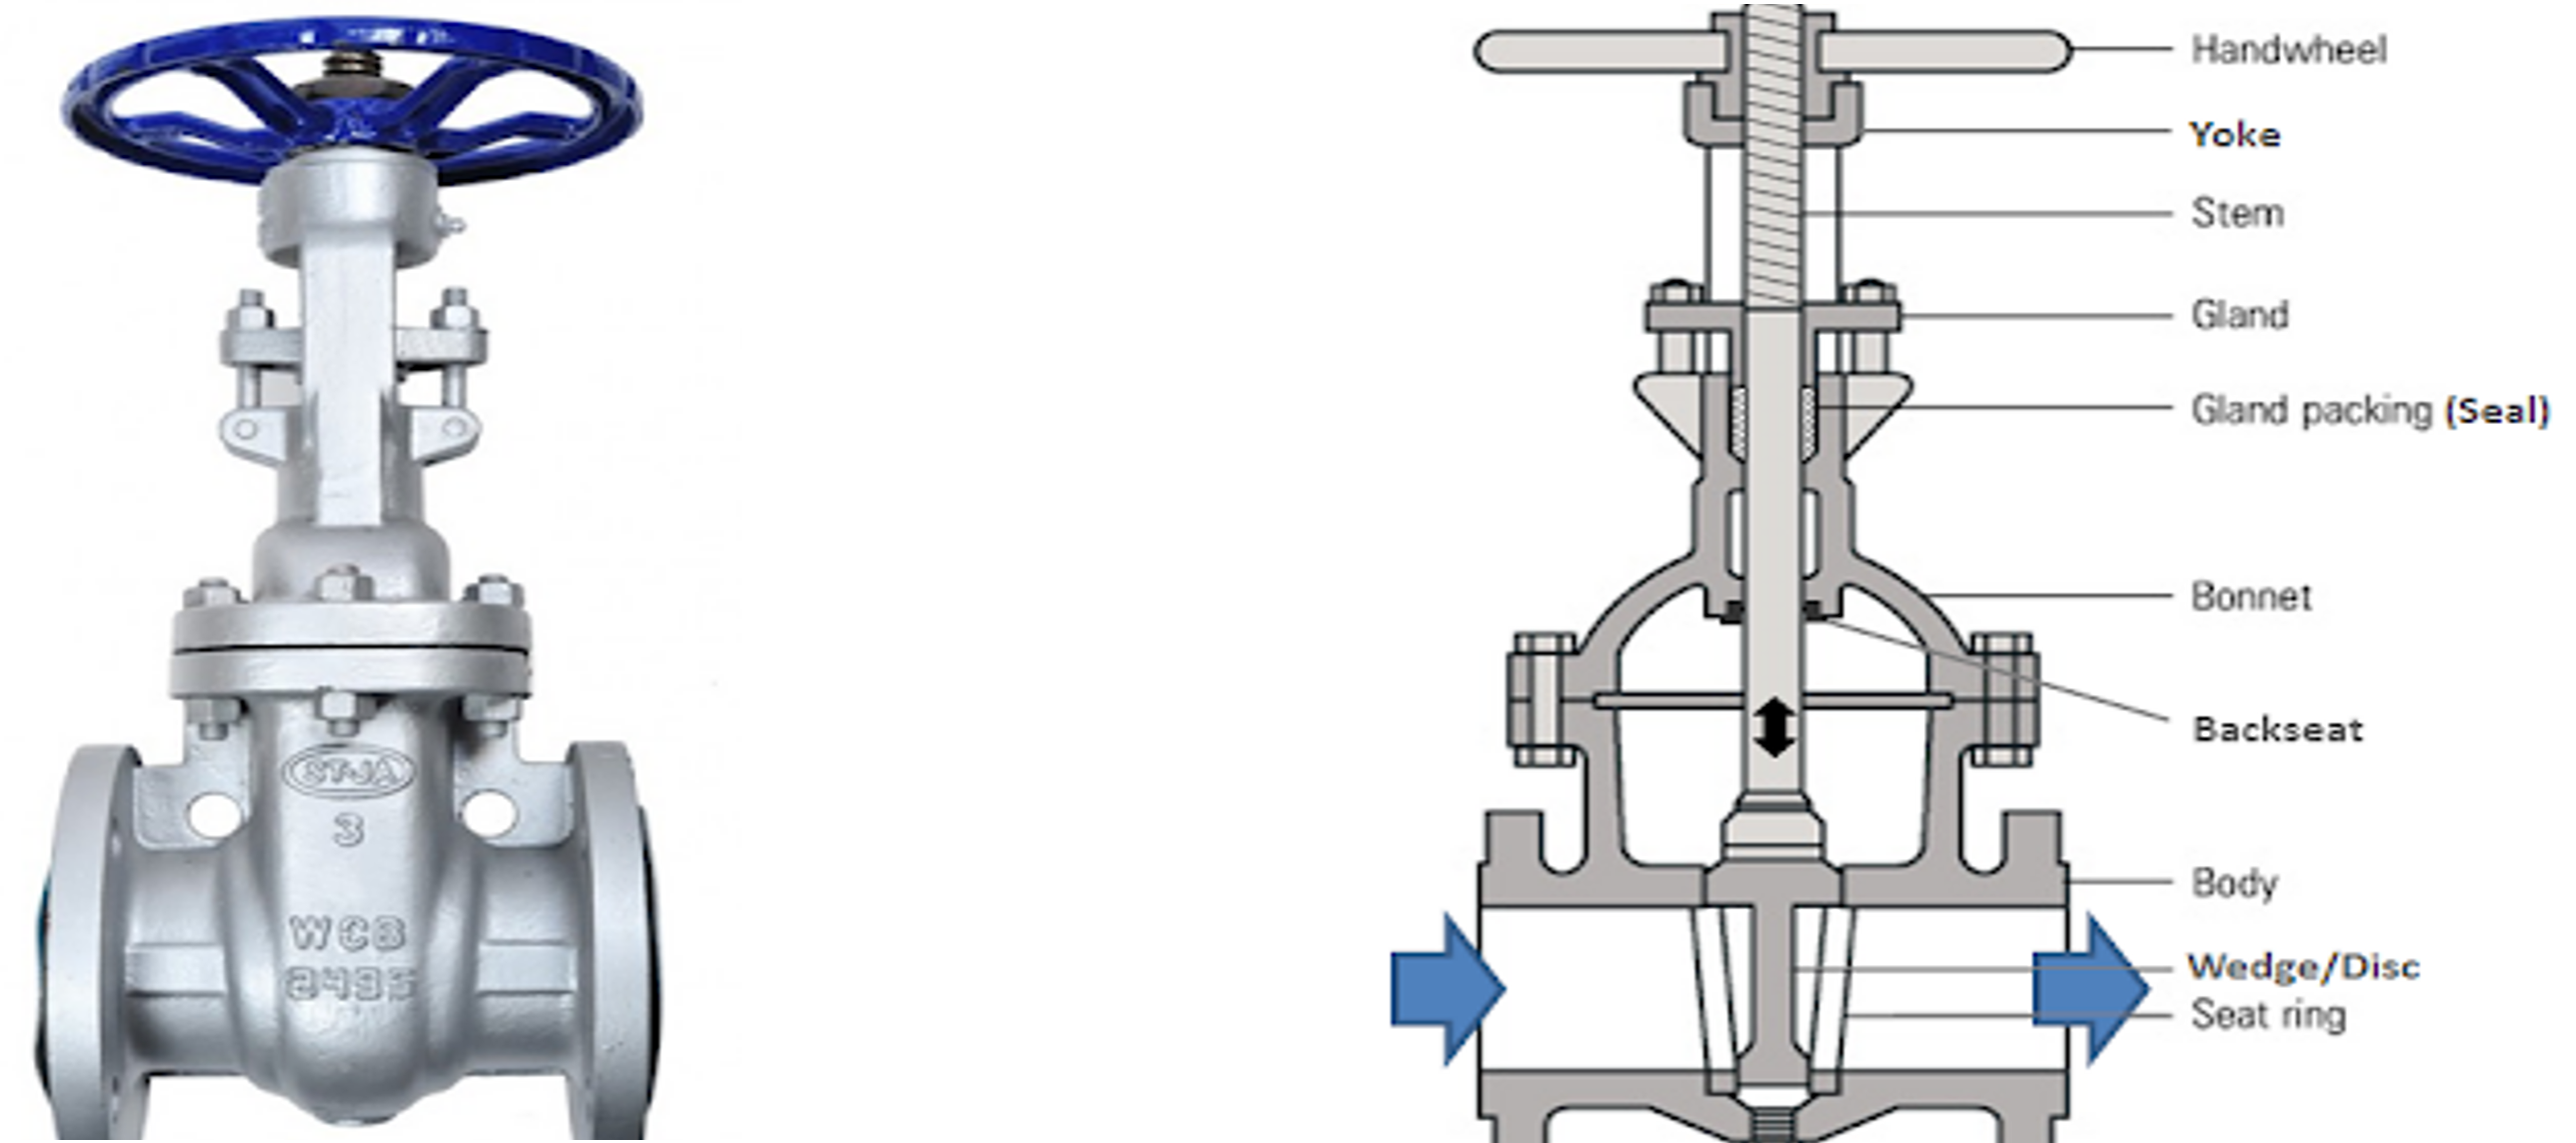
\includegraphics[scale=0.33]{GateValve2.png}\\
    \end{minipage}
    &
            \vspace{0.7cm}
  \scriptsize{\begin{itemize}[topsep=5pt, partopsep=0pt]
  \item Linear stroke type valve \item A gate valve, also known as a sluice valve, is a valve that opens by lifting a barrier (gate) out of the path of the fluid. \item Gate valves require very little space along the pipe axis and hardly restrict the flow of fluid when the gate is fully opened. \item The gate faces can be parallel but are most commonly wedge-shaped (in order to be able to apply pressure on the sealing surface).
  \end{itemize}}  
    &
    %\begin{minipage}[t]{5cm}
        \vspace{0.4cm}
      \begin{itemize}[leftmargin=*]
      \scriptsize{
        \item \textbf{Main application in to isolate sections of mains}
        \item Gate valves are mostly used with larger pipe diameters (from 2" to the largest pipelines) since they are less complex to construct than other types of valves in large sizes. \item Gate valves should not be used to throttle flow as the high velocity of water through a small valve opening can cause cavitation and scour damage to the valve. }
      \end{itemize}
    %\end{minipage}
  
    \\ \hline
   \end{tabular}
\caption{Flow control and isolation valves - Table 1 of 2}
   \label{table:Valve1}  
\end{table}

\end{landscape}

\newpage
\thispagestyle{empty}
\begin{landscape}

   \vspace{-2em} 
\begin{table}
  \centering
  \begin{tabular}{| m{7cm} m{10cm} | m{7cm} | }
    \hline
\multicolumn{2}{c}{Butterfly Valve} & \multicolumn{1}{c}{Use} \\ \hline
    \begin{minipage}{.5\textwidth}
    \begin{center}
%    \tcbox[colframe=green!30!black,
%           colback=green!30]{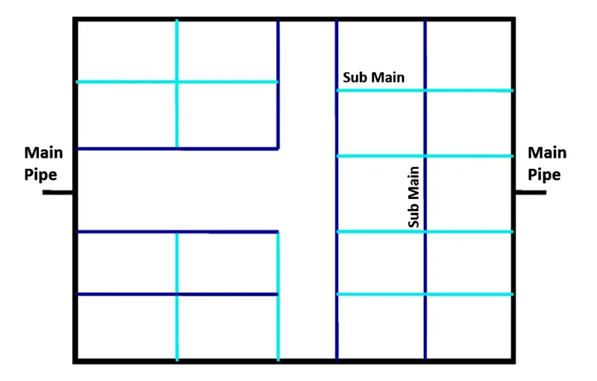
\includegraphics[scale=0.5]{RingDistributionSystem}}    
     \includegraphics[scale=0.25]{ButterflyValve1}\\
     \end{center}
    \end{minipage}
    &
  \scriptsize{\begin{itemize}[topsep=5pt, partopsep=0pt]
  \item Rotary stroke type valve \item Butterfly valves are a family of quarter-turn rotational motion valves that are used in pipelines to shut-off flow. \item The butterfly valve has a disc gate to stop or throttle fluid flow.   \item When closed, the disc seats against a rubber-like seal set into the valve body.  \item In the closed position, the disc blocks the valve bore while in the open position, the disc is oriented perpendicular to the flow direction to allow flow.
  \end{itemize}}  
    &
    %\begin{minipage}[t]{5cm}
      \begin{itemize}[leftmargin=*]
      \scriptsize{
        \item Butterfly valves offer some restriction to flow, which increases headloss. \item However, they are much easier to open and close in large lines than gate valves. \item The butterfly valve is not 100 \% watertight when closed.  \item Typically used as a shut-off valve and not for regulating flow.}
      \end{itemize}
    %\end{minipage}
  
    \\ \hline

\multicolumn{2}{c}{Ball Valve} & \multicolumn{1}{c}{Use} \\ \hline
    \begin{minipage}{.3\textwidth}
%    \tcbox[colframe=green!30!black,
%           colback=green!30]{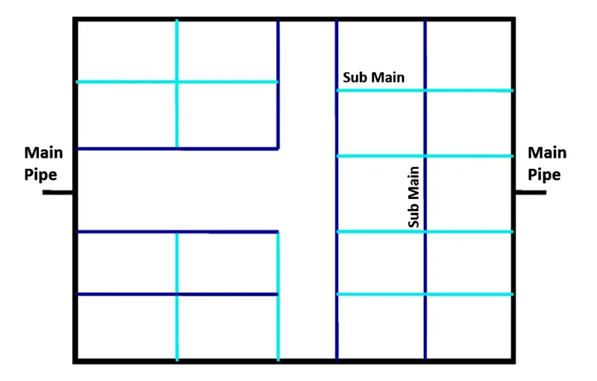
\includegraphics[scale=0.5]{RingDistributionSystem}}    
   \vspace{-2em} 
     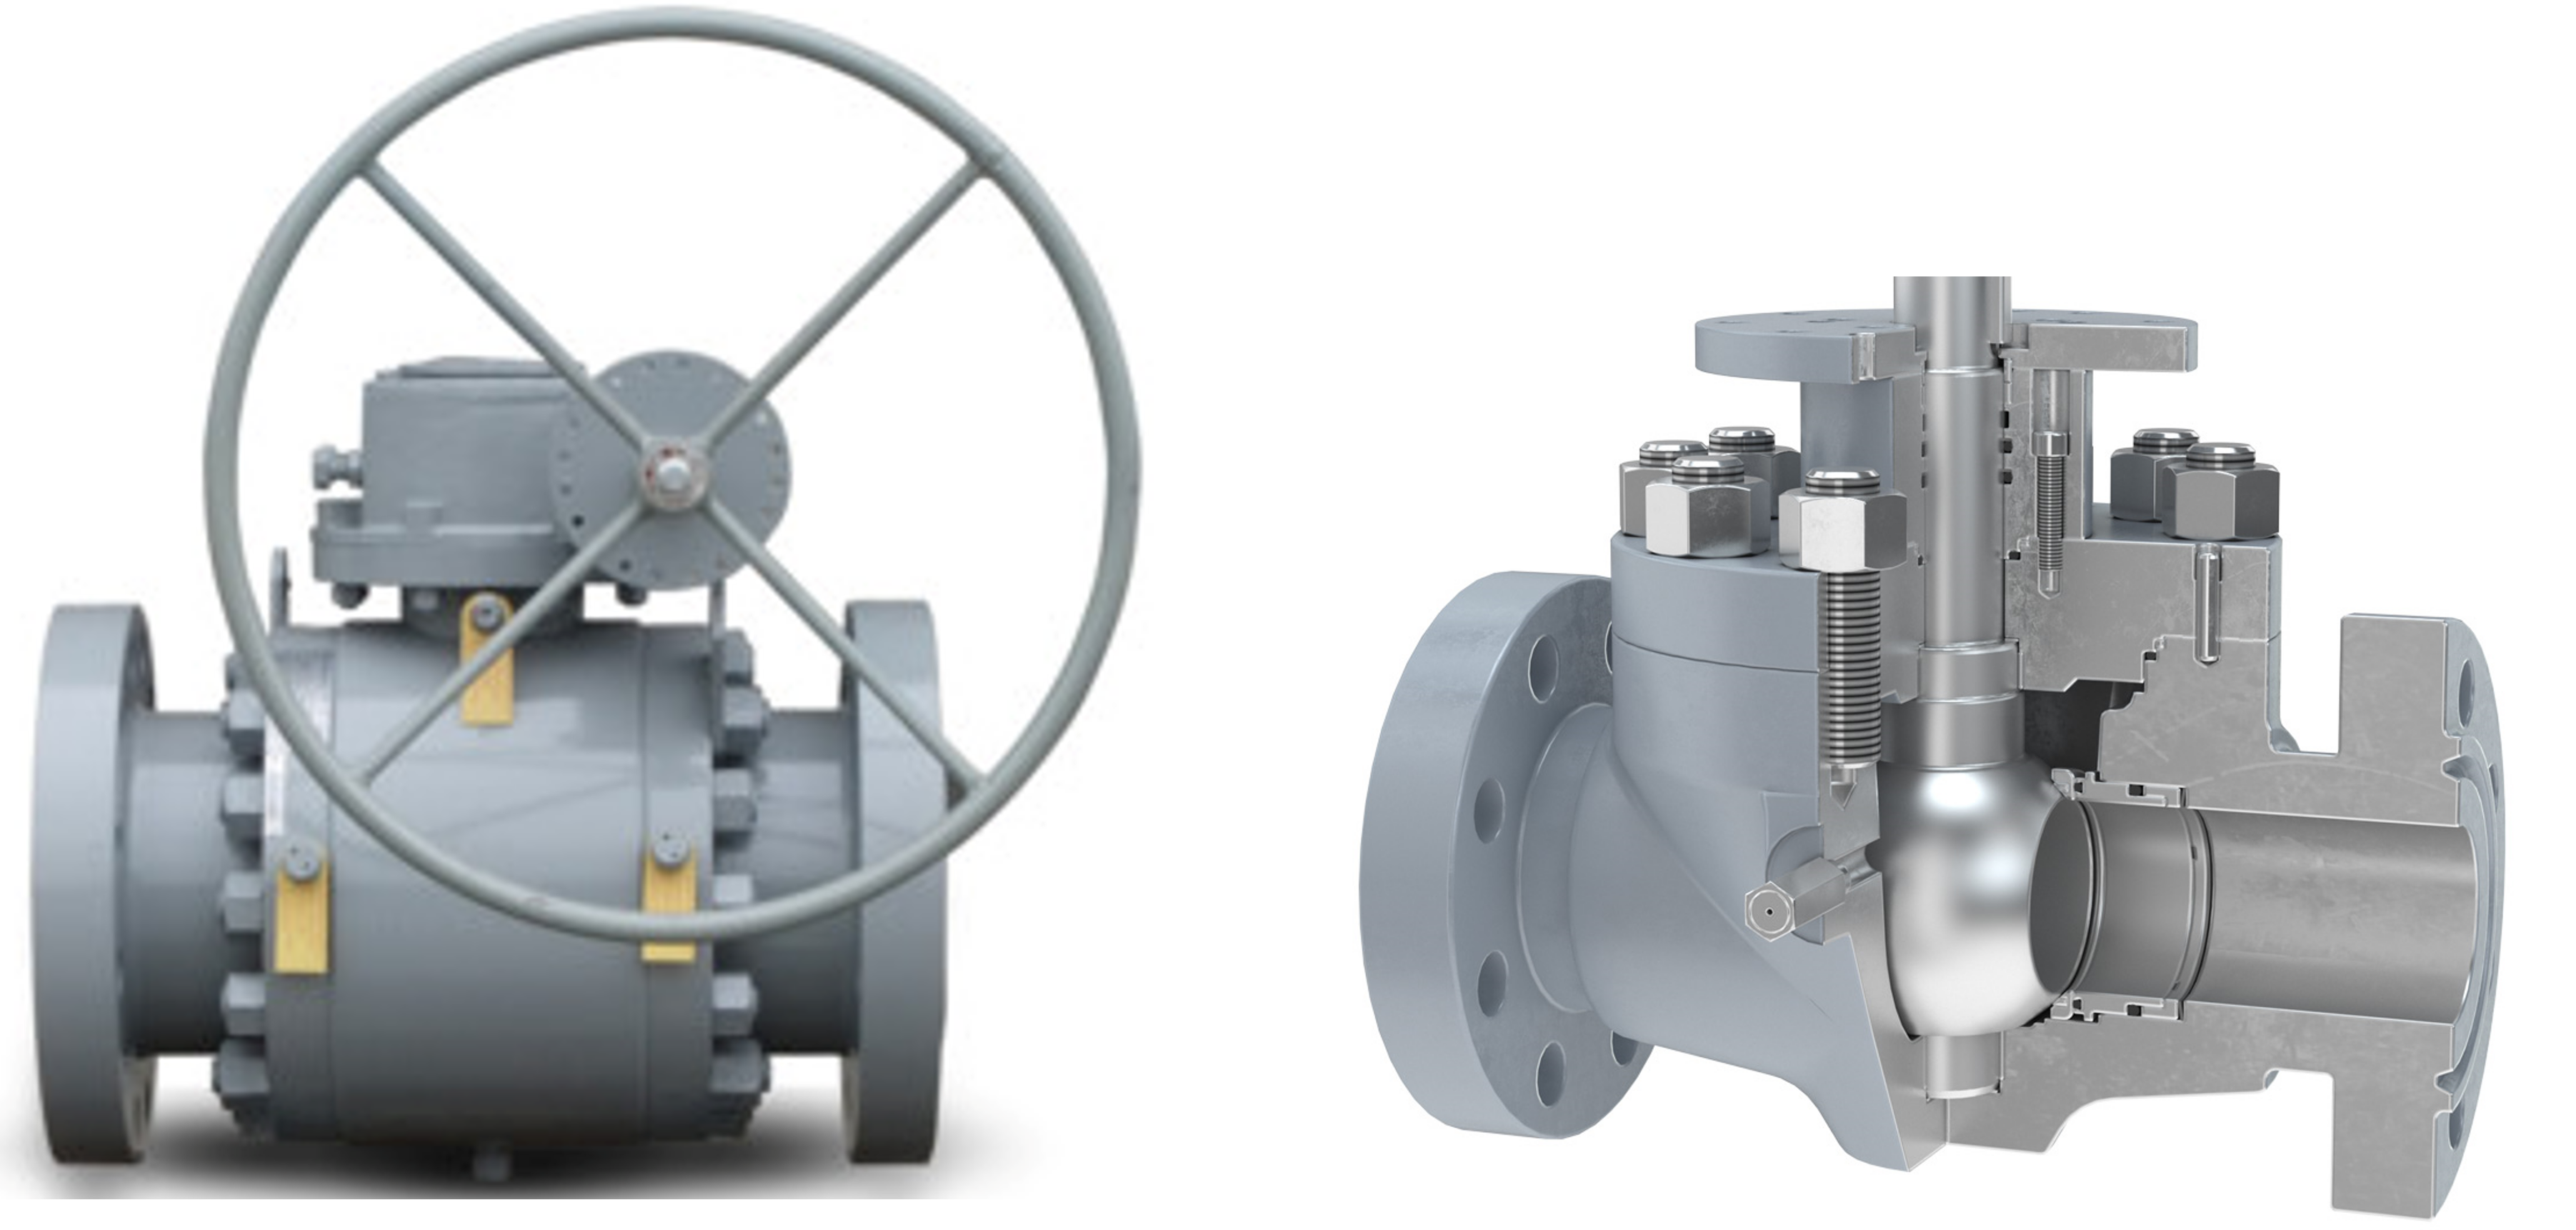
\includegraphics[scale=0.25]{BallValve2}\\
    \end{minipage}
    &
  \scriptsize{\begin{itemize}[topsep=5pt, partopsep=0pt]
  \item Rotary stroke type valve \item Typically used as a shut-off valve. \item Water flow is controlled through a rotational ball containing a hole through its centre placed in the middle of the valve. \item When the ball’s hole is parallel to the water inlet, water can flow through.  When the hole is rotated a quarter turn - 90\si{\degree} to the pipe the passage is blocked, and water cannot flow through.
    \end{itemize}}  
    &
    %\begin{minipage}[t]{5cm}
        \vspace{0.4cm}
      \begin{itemize}[leftmargin=*]
      \scriptsize{
        \item Ball valves are durable, performing well after many cycles, and reliable, closing securely even after long periods of disuse.  }
      \end{itemize}
    %\end{minipage}
  
    \\ \hline
\multicolumn{2}{c}{Foot Valve} & \multicolumn{1}{c}{Use}\\ \hline
    \begin{minipage}{.3\textwidth}
%    \tcbox[colframe=green!30!black,
%           colback=green!30]{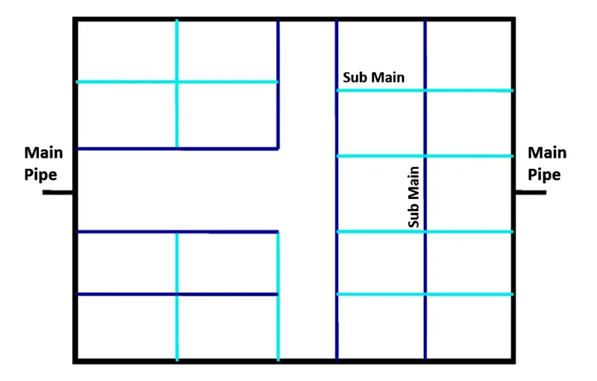
\includegraphics[scale=0.5]{RingDistributionSystem}}    
   \vspace{-2em} 
     \includegraphics[scale=0.35]{FootValve1}\\
    \end{minipage}
    &
  \scriptsize{\begin{itemize}[topsep=5pt, partopsep=0pt]
  \item Linear stroke type valve \item While the pump is running, there’s a constant column of water in the pipe as a result of the suction that’s created. But when the pump is shut off, the suction disappears, the water will flow downward through the pipe because of gravity, back to its original source. The pipe would be left empty of water, instead filled with air.\item Foot valve is a check valve which helps prevent draining of the pump suction pipe after the pump is turned off keeping the pump primed. \item Foot valves open in one direction and close off when the direction of flow is reversed. That means that in an application such as pumping from a well, the water can only be extracted out of the well. 

  \end{itemize}}  
    &
    %\begin{minipage}[t]{5cm}
        \vspace{0.4cm}
      \begin{itemize}[leftmargin=*]
      \scriptsize{
        \item Foot valves are used for suction lift applications, like a well pump. help keep a pump primed therefor stopping your pump from burning out.}
      \end{itemize}
    %\end{minipage}
  
    \\ \hline
   \end{tabular}
   \caption{Flow control and isolation valves - Table 2 of 2} 
      \label{table:Valve2}  
\end{table}

\end{landscape}

\subsection{Air Valves}\index{Air valves}

  \begin{itemize}
   \item Air valves are an essential component of the water supply system
\item Air and vacuum formed in water mains may lead to serious operating problems and even some dramatic consequences. Air can enter piping systems in several ways:
\begin{itemize}
\item Empty Pipelines:  Pipelines not in operations are occupied with air. Most of it is evacuated during startup, but some air pockets can remain in the system.
 
\item Dissolved air in water: Depending on the temperature and pressure, water can contain trapped or dissolved air. During fluid flow, it separates from the liquid and can become trapped at the system’s high points. Also, in pipelines conveying sewage, the liquid waste can undergo chemical reactions and evolve into gases that can get trapped in the wastewater system.
 
\item Mechanical equipment: Air can also get into the pipeline through mechanical systems like pumps, pipe joints, valves, etc. Leaks or faulty seals in these components.

\end{itemize}
\item Consequences of air and vacuum in pipelines include:
\begin{itemize}
\item Reduced pumping efficiency: Air in pipelines can reduce the efficiency of the pumping system. The air trapped at the high points of the system blocks flow, increasing the pressure head and thus the energy required for flow to occur.
 
\item Pipeline corrosion: Depending on the pipeline's temperature, oxygen in the trapped air can be a powerful corrosive agent. The oxygen oxidizes the metal gradually, which leads to rusting, blockage, and structural failure of the pipe.
 
\item Faulty metering and instrumentation devices: Air pockets and vacuums can cause problems for flow measuring and control devices. They affect the ability of the devices to accurately measure and control the flow.
 
\item Air hammer: When a trapped air pocket is present in a pipe, pressure builds up around the blockage. The pressure of the water swirling around this blockage sends vibrations throughout the pipe. This vibration, known as an air hammer, can potentially damage the distribution system components.
 
\item Pipe failure: Vacuums can cause catastrophic failures in pipelines. If there is a substantial vacuum, the pipe can collapse inwards due to the pressure difference on both sides of the pipe's walls.
\end{itemize}
\item Table ~\ref{table:Airvalve} summarizes the properties and use of the commonly used distribution system air valves and Figure ~\ref{fig:Airvalve1} provides a schematic of the air valve applications.
\end{itemize}

\newpage
\thispagestyle{empty}
\begin{landscape}
\begin{table}[h!]
  \centering
  \begin{tabular}{| m{7cm} m{10cm} | m{7cm} | }
    \hline
\multicolumn{2}{c}{\scriptsize{Air and vacuum valves}} & \multicolumn{1}{c}{\scriptsize{Use}} \\ \hline
    \begin{minipage}{.5\textwidth}
    \begin{center}
    \hspace{0.5cm}
%    \tcbox[colframe=green!30!black,
%           colback=green!30]{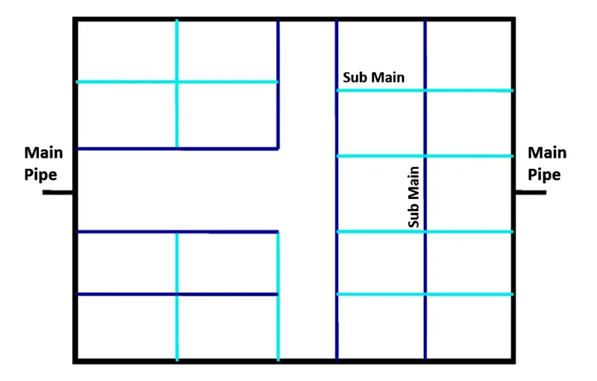
\includegraphics[scale=0.5]{RingDistributionSystem}}    
     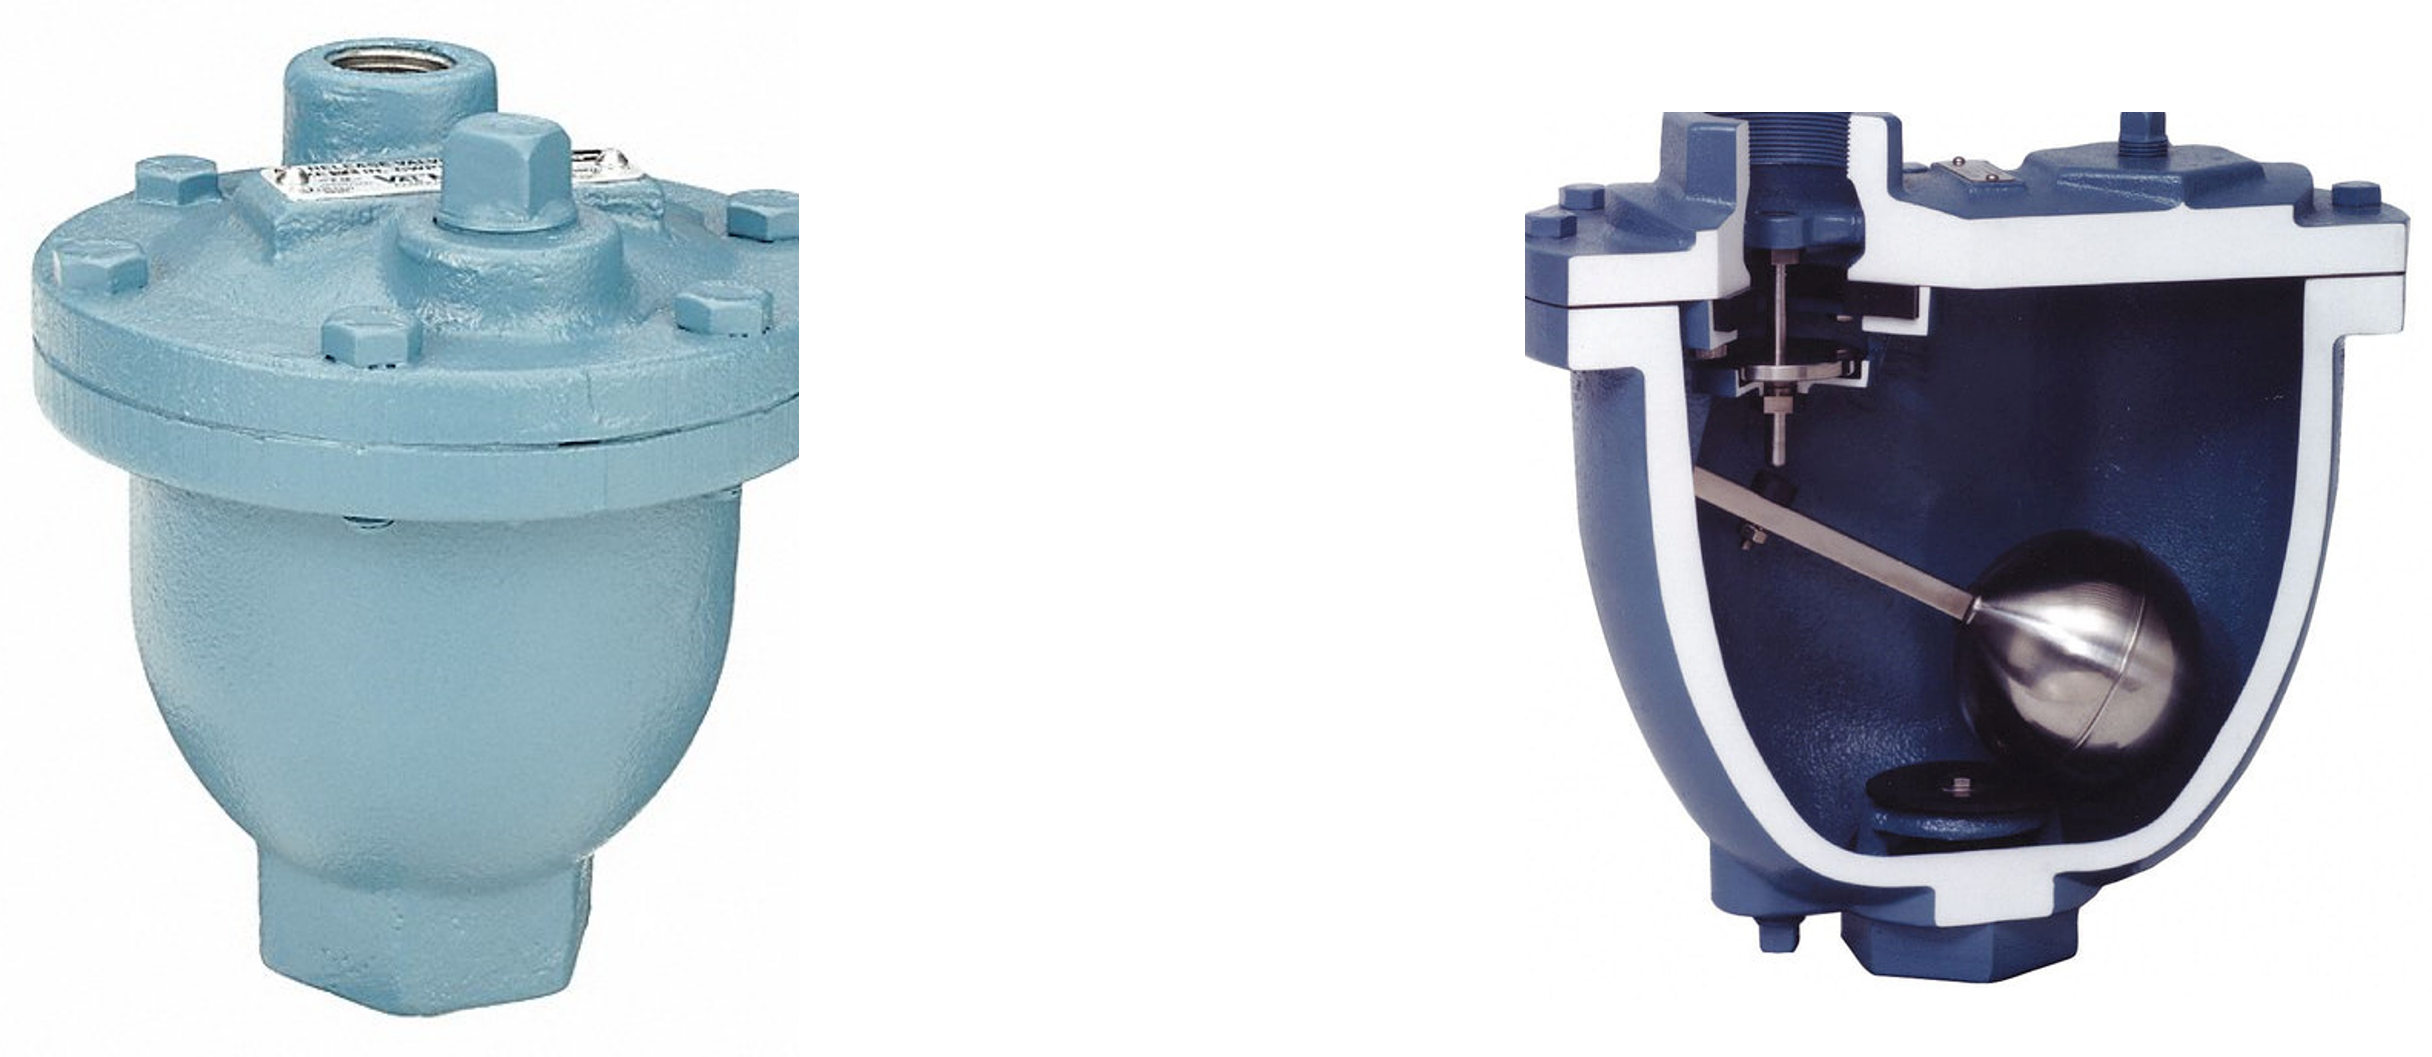
\includegraphics[scale=0.25]{AirVacuumValve1}\\
     \end{center}
    \end{minipage}
    &
  \scriptsize{\begin{itemize}[topsep=5pt, partopsep=0pt]
  \item These float operated valves allow the escape of air while the line is being filled. \item Once the line is filled, the pressure in the valve keeps the valve from opening even if air accumulates in the valve. \item When the line is drained and the internal pressure drops below atmospheric, the valve opens, allowing air in preventing a vacuum and possible pipeline collapse. \item These valves are also referred to as air relief valves.
  \end{itemize}}  
    &
    %\begin{minipage}[t]{5cm}
        \vspace{0.4cm}
      \begin{itemize}[leftmargin=*]
      \scriptsize{
        \item Exhausts large quantities of air at system start-up. \item Provides pipeline vacuum protection. \item Admits large quantities of air to prevent loss of pressure during power failures, line breaks and drainage}
      \end{itemize}
    %\end{minipage}
  
    \\ \hline
\multicolumn{2}{c}{\scriptsize{Air Release Valve}} & \multicolumn{1}{c}{\scriptsize{Use}} \\ \hline
    \begin{minipage}{.3\textwidth}
%    \tcbox[colframe=green!30!black,
%           colback=green!30]{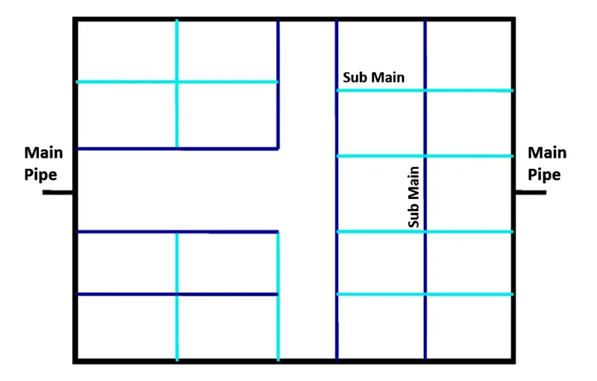
\includegraphics[scale=0.5]{RingDistributionSystem}}    
   \vspace{-0.5em} 
     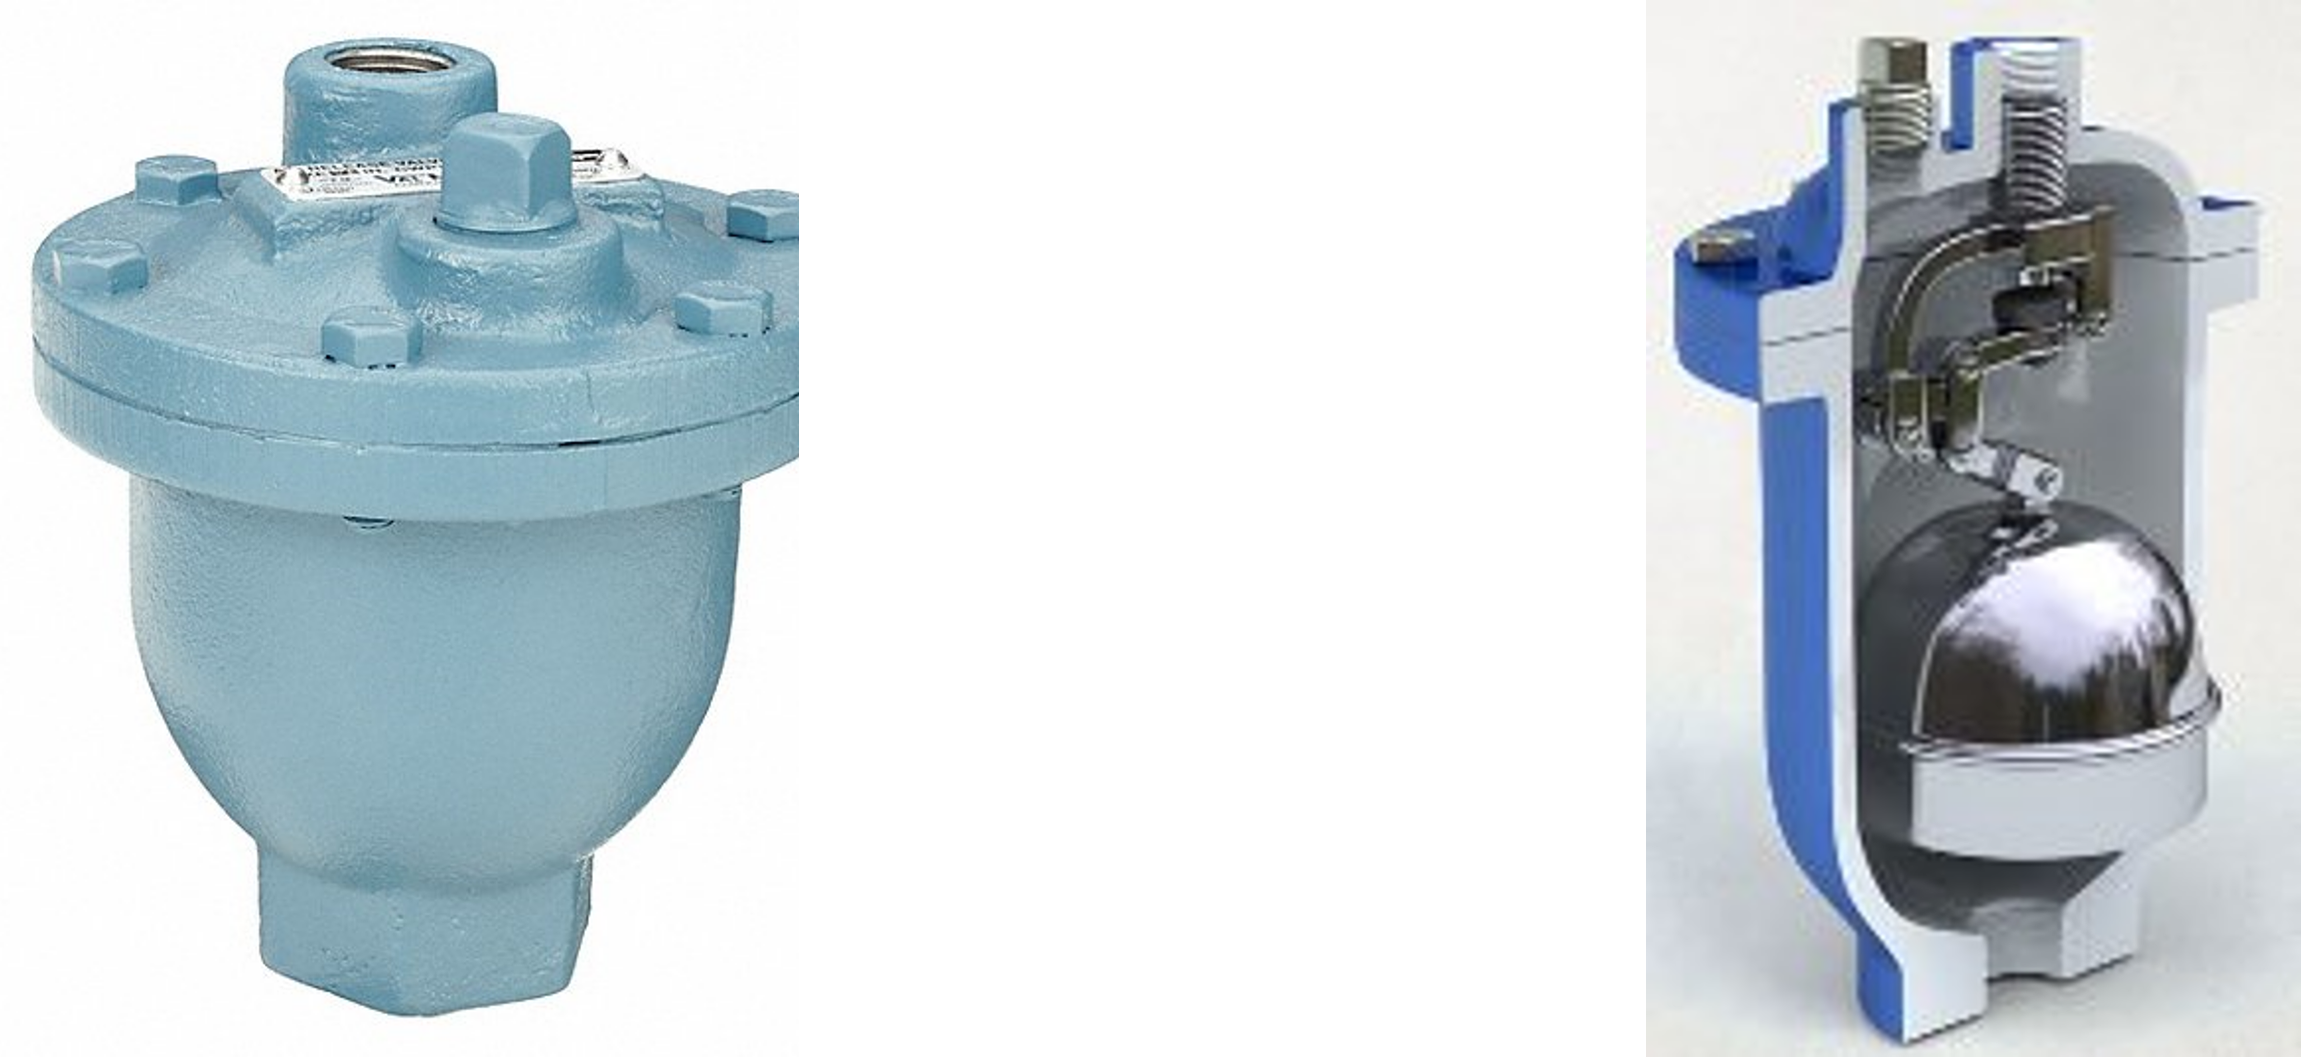
\includegraphics[scale=0.3]{AirReleaseValve3.png}\\
    \end{minipage}
    &
  \scriptsize{Automatic air release valves are installed at the highest points in a pipeline where air naturally collects. Air bubbles enter the valve and displace the liquid inside, lowering the liquid level. When the level drops to where it no longer buoys the float, the float drops. This motion pulls the seat away from the orifice, triggering the valve to open and vent the accumulated air into the atmosphere.
}  
    &
    %\begin{minipage}[t]{5cm}
        \vspace{0.4cm}
      \begin{itemize}[leftmargin=*]
      \scriptsize{
        \item Air is from: the pipeline itself,  air dissolved in the water pumped and drawn in from equipment like pumps, joints etc. \item Prevents pressure surges, water hammer and prevent flow stoppage due to air binding.}
      \end{itemize}
    %\end{minipage}
  
    \\ \hline
\multicolumn{2}{c}{\scriptsize{Combination Valves}} & \multicolumn{1}{c}{\scriptsize{Use}}\\ \hline
    \begin{minipage}{.3\textwidth}
%    \tcbox[colframe=green!30!black,
%           colback=green!30]{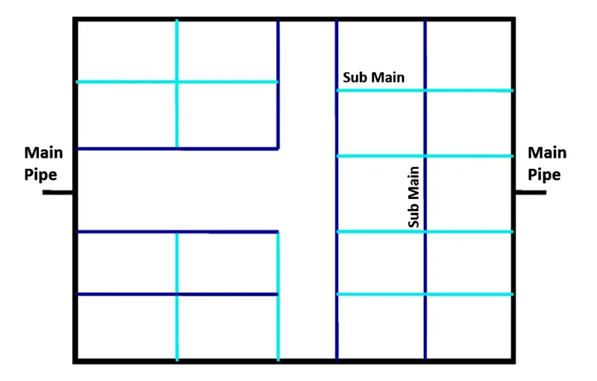
\includegraphics[scale=0.5]{RingDistributionSystem}}    
   \vspace{-2em} 
     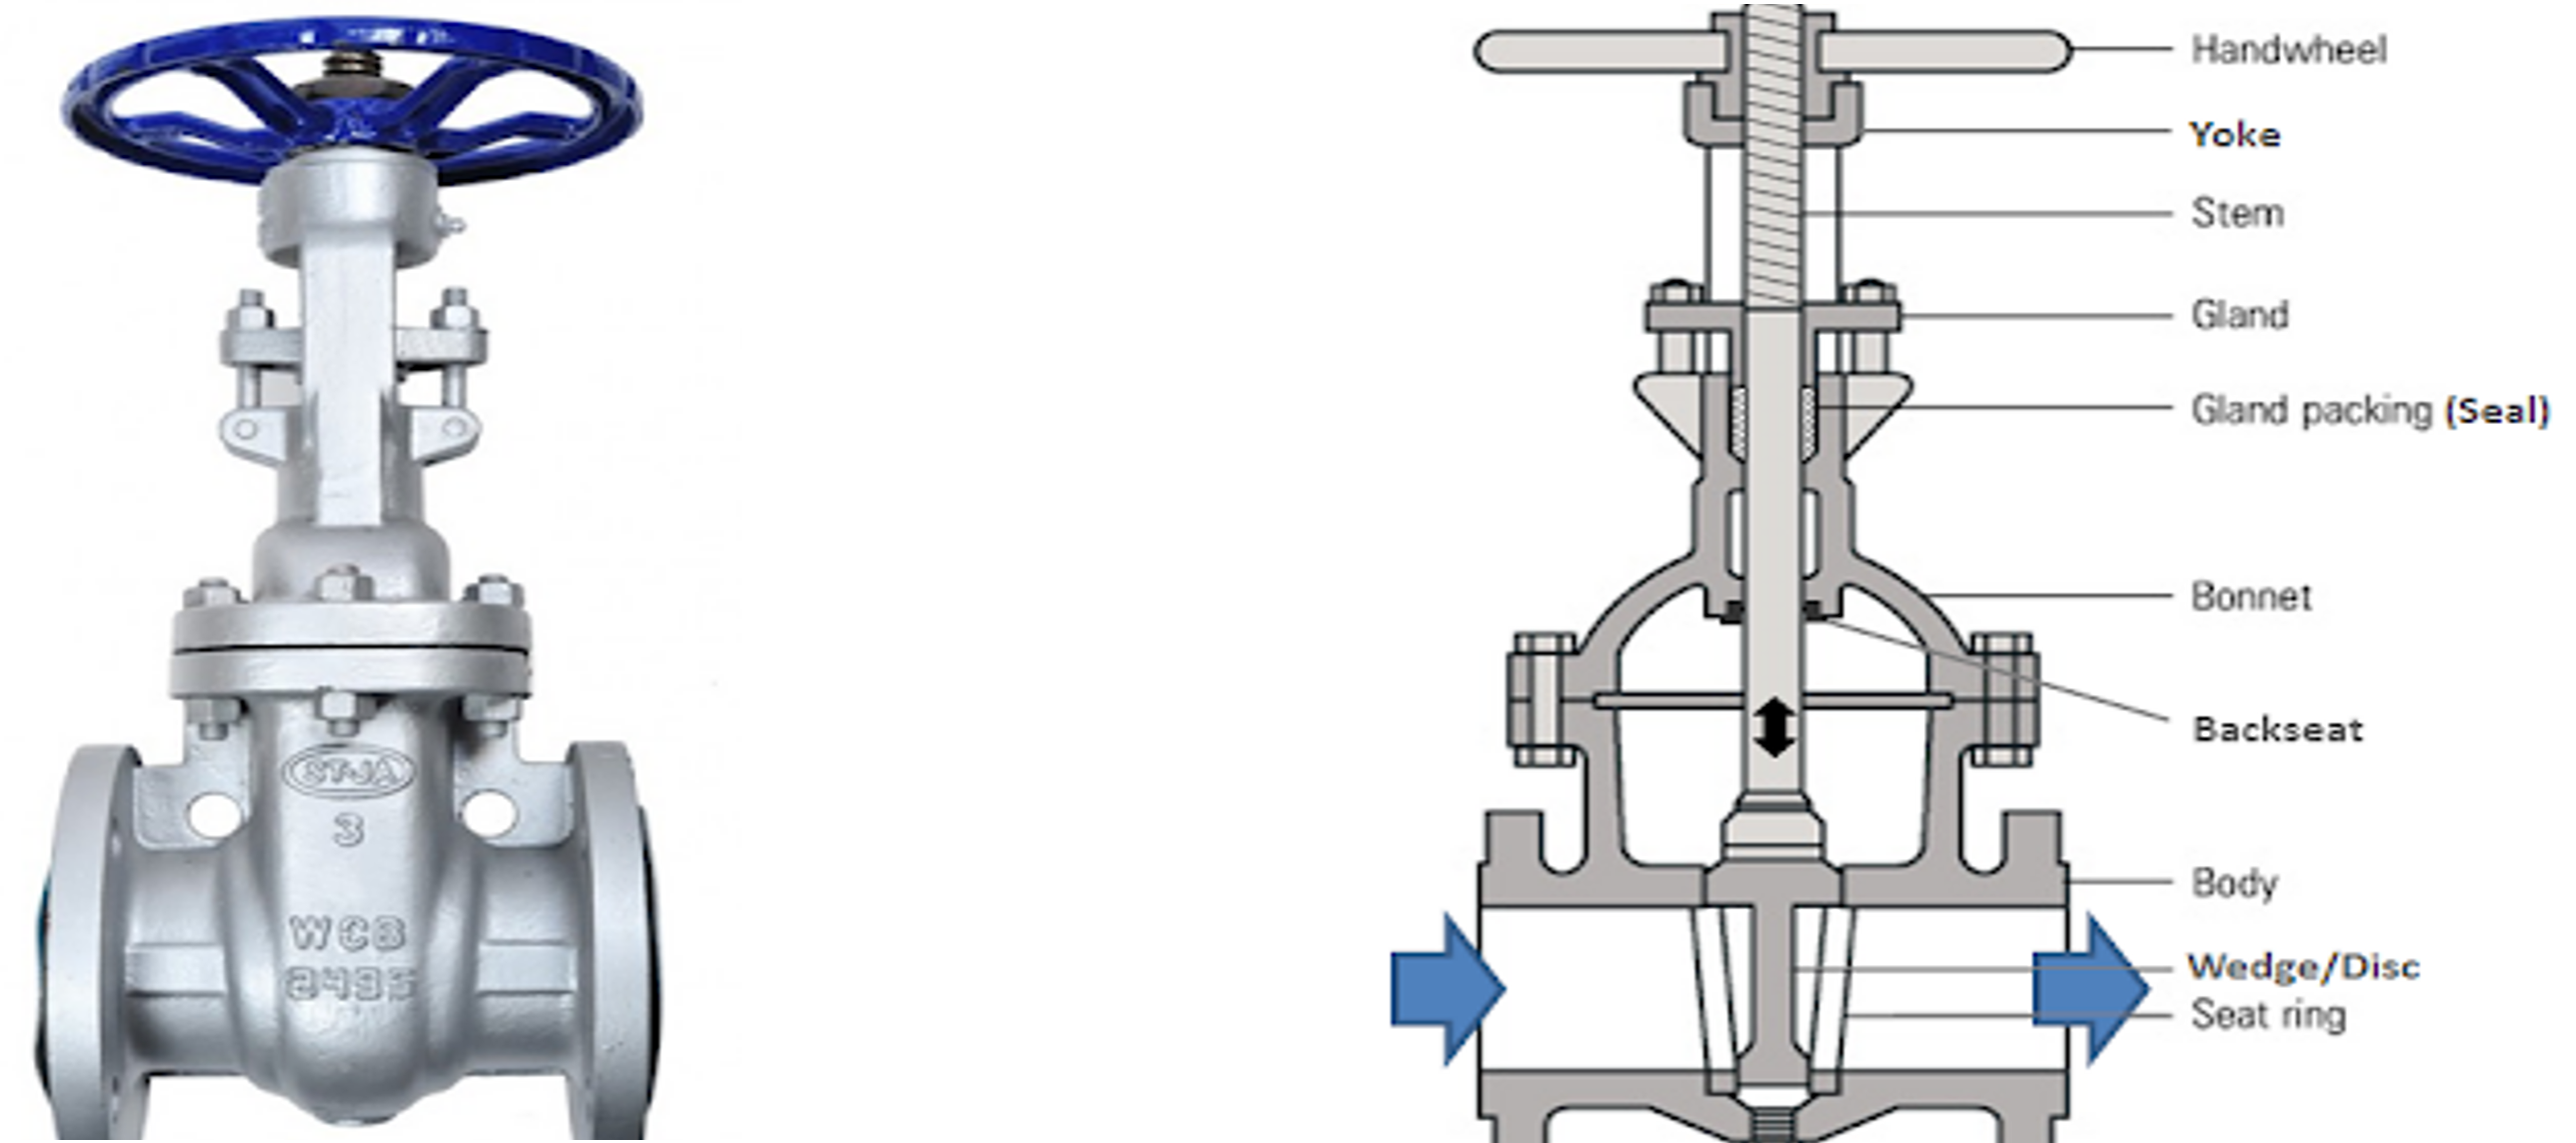
\includegraphics[scale=0.3]{GateValve2.png}\\
    \end{minipage}
    &
\phantom{\tiny{Phantom}}   \vspace{-1em}
  \scriptsize{\begin{itemize}\setlength\itemsep{1em}
  \item There are two types of combination valves. \begin{enumerate} \item The most common is the combination of air release and vacuum relief often referred to simply as an air vac valve. \item The second combination valve is one designed with two orifices, one for high airflow and one for low airflow.\end{enumerate} \item Combination air vac valves are installed at high points in the line to allow air in and out of the line to reduce problems due to a blockage by air. \item Allowing air when the line may be being emptied prevents the low internal pressure from drawing a joint gasket into the pipe and thus causing a leak..
  \end{itemize}}  
    &
    %\begin{minipage}[t]{5cm}
        \vspace{0.4cm}
      \begin{itemize}[leftmargin=*]
      \scriptsize{
        \item Gate valves are used to shut off the flow of liquids rather than for flow regulation. \item Gate valves are mostly used with larger pipe diameters (from 2" to the largest pipelines) since they are less complex to construct than other types of valves in large sizes. }
      \end{itemize}
    %\end{minipage}
  
    \\ \hline
   \end{tabular}
     \caption{Air valves in water system}
                \label{table:Airvalve} 
\end{table}

\end{landscape}



\thispagestyle{empty}
\begin{landscape}
 \vspace{3cm}
\hspace{1cm}
\begin{figure}
     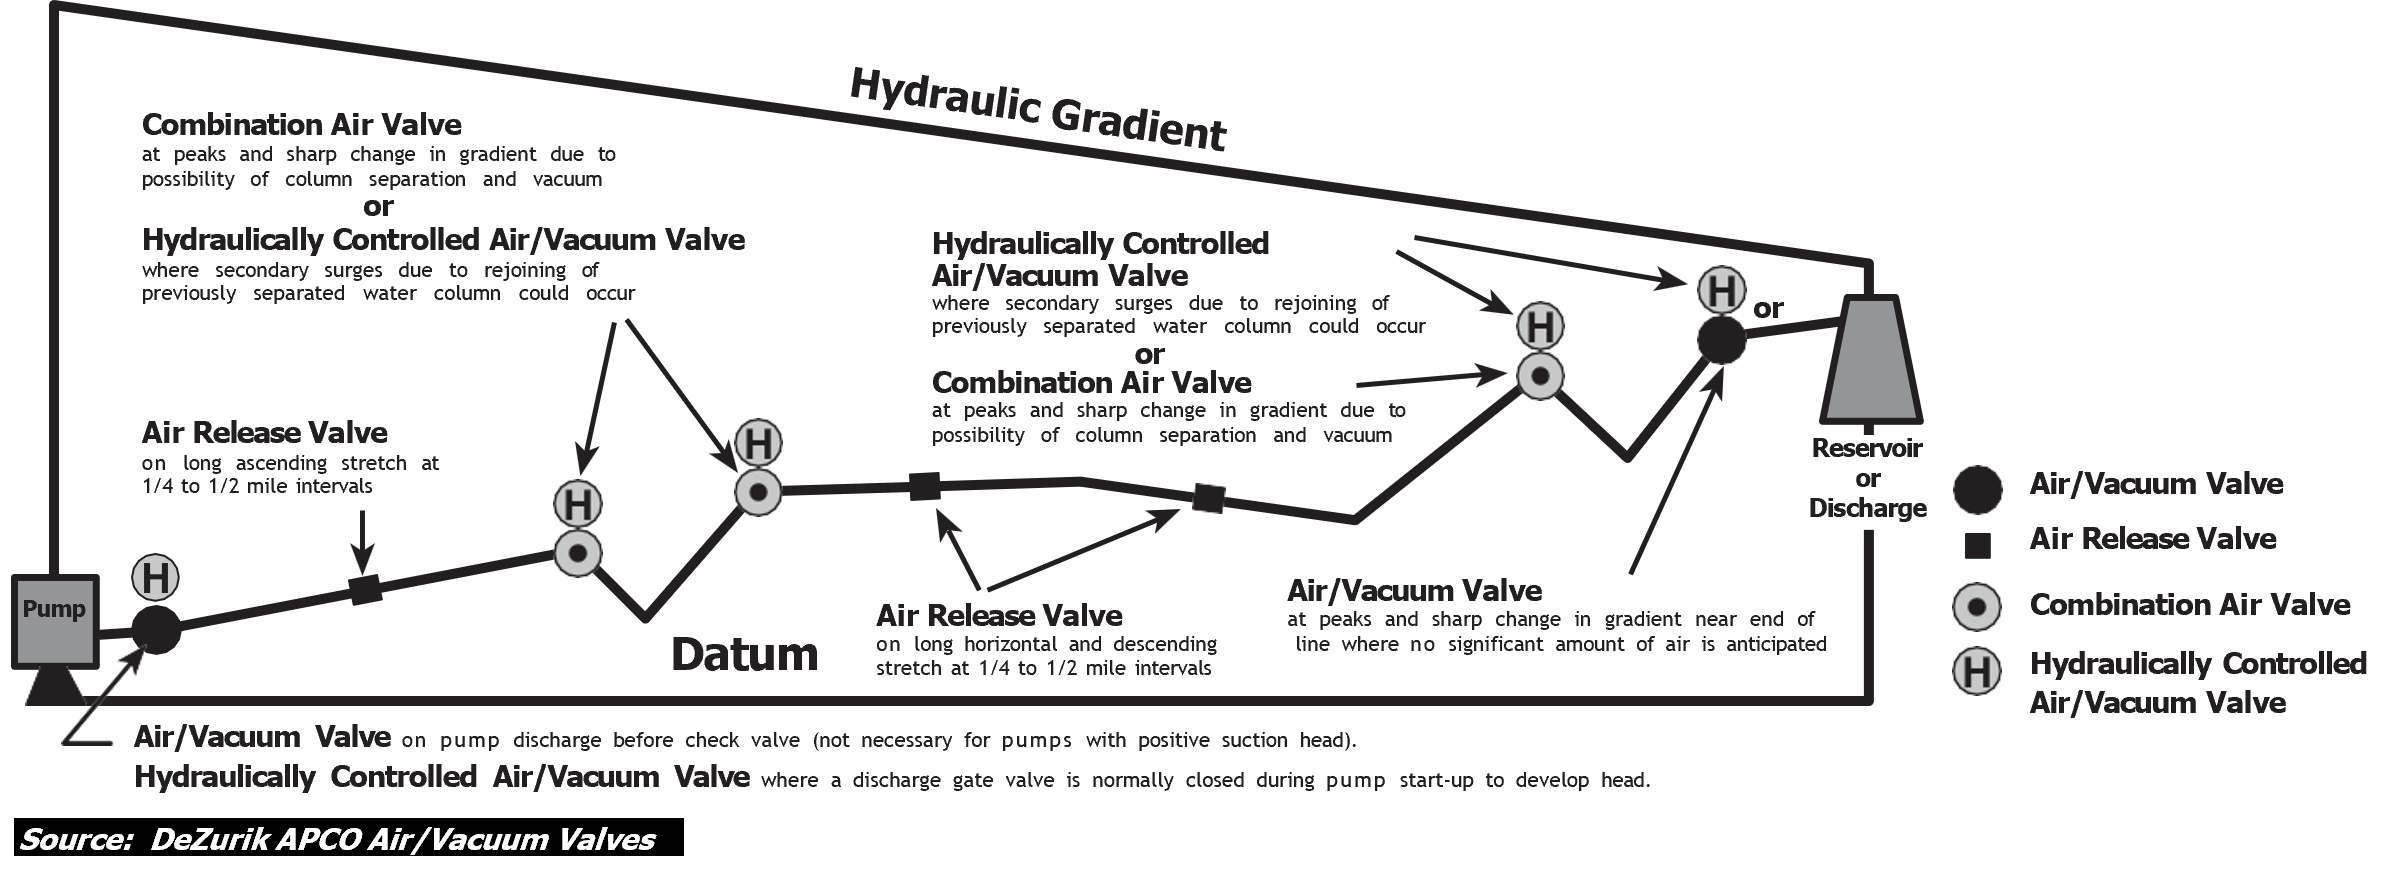
\includegraphics[scale=1.35]{AirValvesApplication}
     \caption{Summary of air valve applications}
\label{fig:Airvalve1}
     \end{figure}
     \end{landscape}

\subsection{Backflow Prevention}\index{Backflow}
\begin{itemize}[itemsep=0.5em,parsep=-0.5em]
\item Backflow means the undesirable reversal of flow of a liquid, gas, or suspended solid into the potable water supply.
\item A backflow preventer is designed to keep this from happening. 
\item Points at which a potable water system connects with a non-potable water system are called cross connections. Such connections occur naturally in appliances such as clothes washers and dishwashers, but they must be carefully designed and installed to prevent backflow. 
\item Back-siphonage:\index{Backflow!Back siphonage}
\begin{itemize}
\item This is when higher pressure fluids, gases, or suspended solids move to an area of lower pressure fluids. A significant drop of pressure in a water delivery system creates a similar suction, pulling possibly undesirable material into the system. The effect is similar to drinking water through a straw. 
\item This is an example of an indirect cross-connection.\index{Backflow!Indirect cross-connection}
\end{itemize}

\item Back-pressure: \index{Backflow!Back-pressure}
\begin{itemize}
\item Occurs when a fluid under a higher pressure from systems like boilers, heat exchanging equipment, power washing equipment, fire sprinklers, or pumps enter potable water piping. This is an example of a \colorbox{green}{direct cross-connection}, with undesirable material being pushed into the system.
\end{itemize}
\item To reduce the risk of contamination, a backflow preventer can be fitted. A backflow preventer is also important when potentially toxic chemicals are used, for instance for commercial/industrial descaling of boilers, or when chemical bleaches are used for residential power washing.
\item Another common location for a backflow preventer is the connection of a fire sprinkler system to a water main, to prevent pressurized water from flowing from the fire suppression system into the public water supply. \index{Backflow!Backflow preventer}
\item Backflow preventers are categorized into three groupings: Assembly, Device or Method. 
\item Tables ~\ref{table:Backflow1} and ~\ref{table:Backflow2} summarize the properties and use of the commonly used backflow devices. 
\end{itemize}

\newpage
\thispagestyle{empty}
\begin{landscape}
\begin{table}[h!]
  \begin{tabular}{|c m{20cm} |}
    \hline
\multicolumn{2}{c}{Air Gap} \index{Backflow!Prevention devices!Air gap}\\ \hline
    \begin{minipage}{.3\textwidth}
    \hspace{1cm}
%    \tcbox[colframe=green!30!black,
%           colback=green!30]{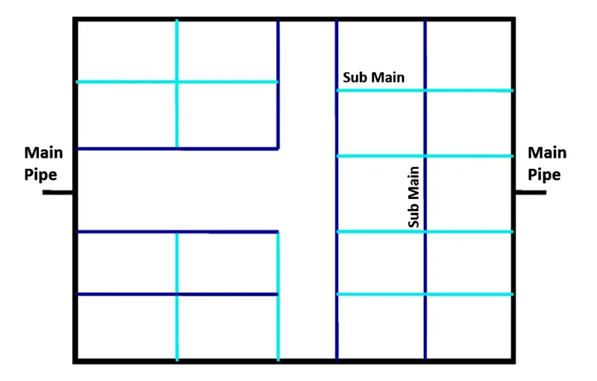
\includegraphics[scale=0.5]{RingDistributionSystem}}    
     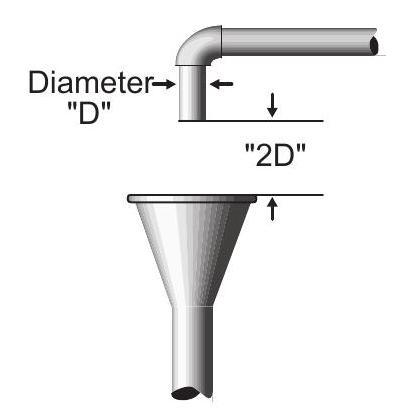
\includegraphics[scale=0.16]{AirGap}\\
    \end{minipage}
     &
    \vspace{0.3cm}
    %\begin{minipage}[t]{5cm}
\scriptsize{\begin{itemize}[topsep=5pt, partopsep=0pt]
\item A physical separation between the free-flowing discharge end of a potable water supply pipeline and an open or non-pressure receiving vessel. 
\item Should not be used in an area with dangerous atmosphere.
\item An "approved air gap" shall be at least twice the diameter of the supply pipe measured vertically above the overflow rim of the receiving vessel; in no case less than 1 inch $(2.54 \mathrm{~cm})$.

\textbf{Common Applications - Lethal hazards (raw sewage, recycled water, auxiliary water supply}
\end{itemize}}
\\ \hline

\multicolumn{2}{c}{Atmospheric Vacuum Breaker Assembly (AVB)}\\ \hline \index{Backflow!Prevention devices!Atmospheric vacuum breaker assembly (AVB) }
    \begin{minipage}{.3\textwidth}
%    \tcbox[colframe=green!30!black,
%           colback=green!30]{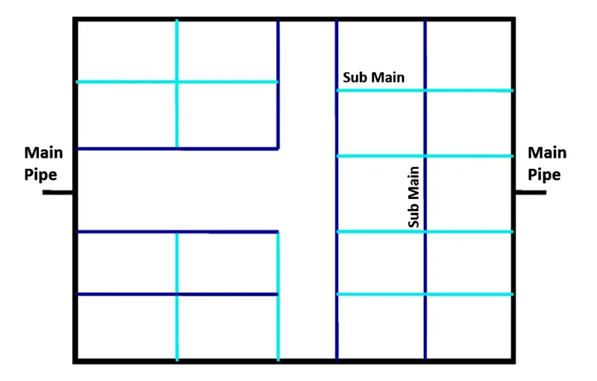
\includegraphics[scale=0.5]{RingDistributionSystem}}    
     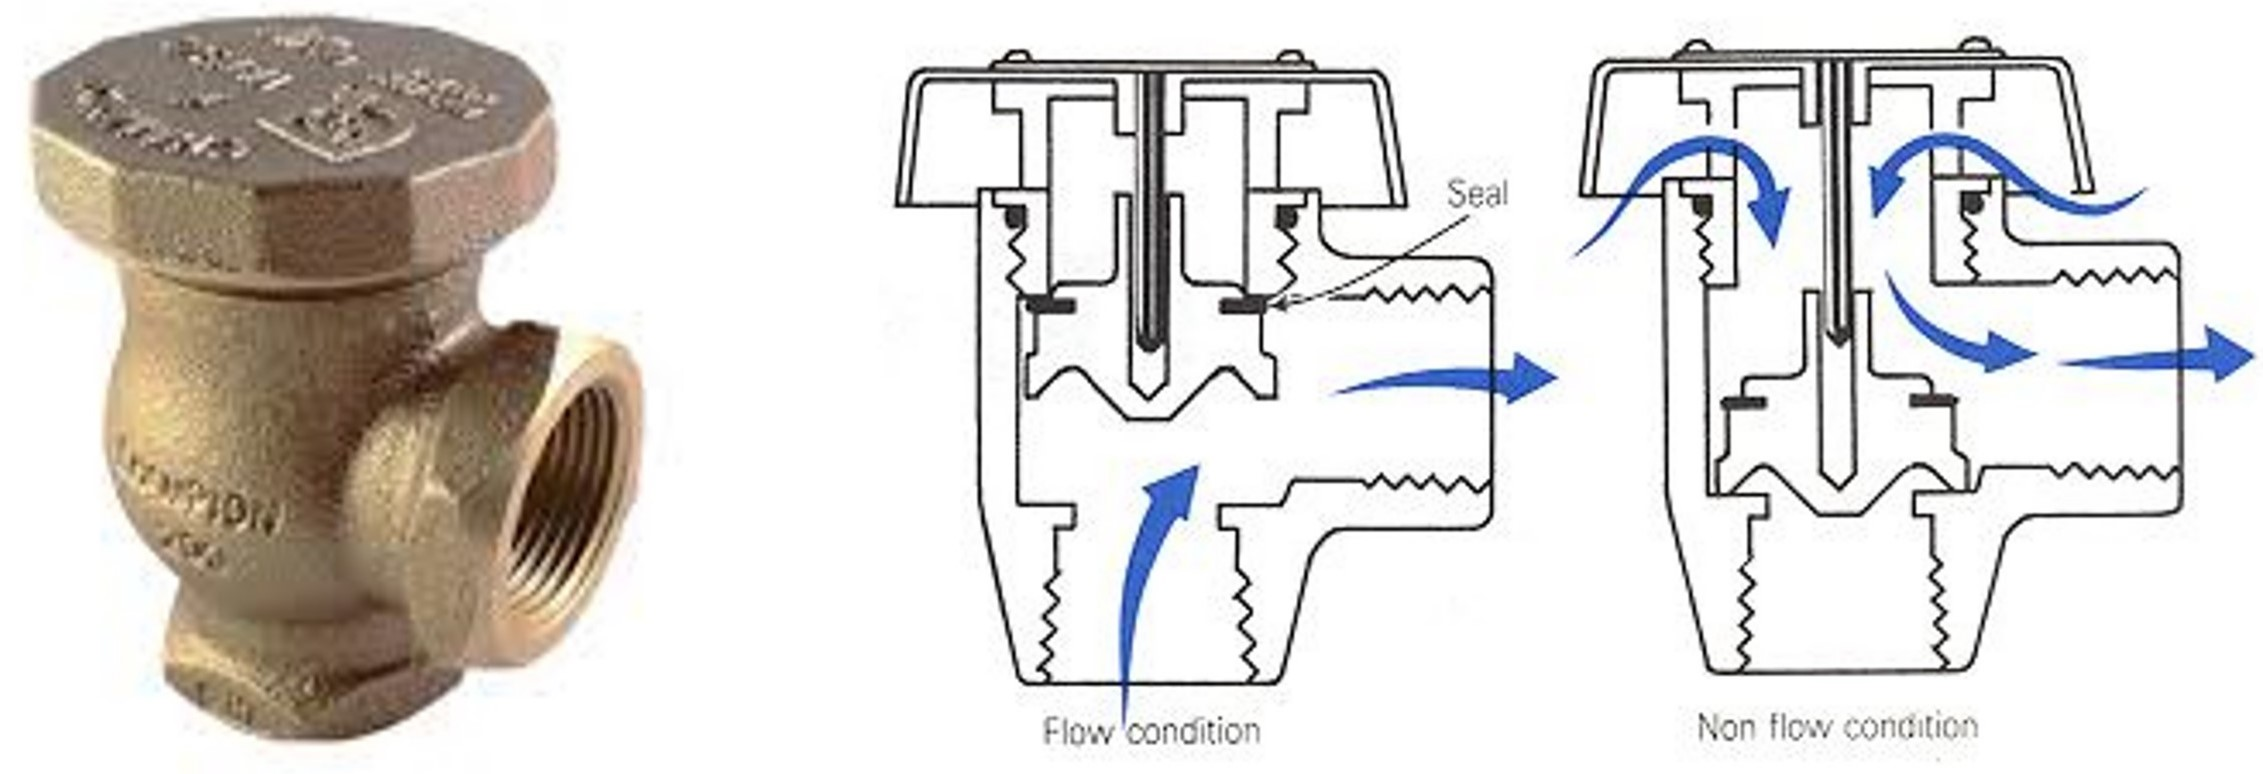
\includegraphics[scale=0.32]{AtmosphericVacuumBreaker(3)}\\
    \end{minipage}
     &
    \vspace{0.3cm}
    %\begin{minipage}[t]{5cm}
\scriptsize{\begin{itemize}[topsep=5pt, partopsep=0pt]
\item Also known as the non-pressure type vacuum breaker, it consists of an air inlet valve, a check seat and an air inlet port(s). (.) The flow of water into the body causes the air inlet valve to close the air inlet port(s). 
\item When the flow of water stops the air inlet valve falls and forms a check valve against backsiphonage. At the same time it opens the air inlet port(s) allowing air to enter and satisfy the vacuum. 
\item A shutoff valve immediately upstream may be an integral part of the assembly, but there shall be no shutoff valves or obstructions downstream. 
\item An atmospheric vacuum breaker is designed to protect against a non-health hazard (i.e., pollutant) or a health hazard (i.e., contaminant) under a back-siphonage condition only.

\textbf{Common Applications - Irrigation systems}


\end{itemize}}
    %\end{minipage}
    
    \\ \hline
\multicolumn{2}{c}{Spill Resistant Vacuum Breaker} \index{Backflow!Prevention devices!Spill resistant vacuum breaker}\\ \hline
    \begin{minipage}{.3\textwidth}
%    \tcbox[colframe=green!30!black,
%           colback=green!30]{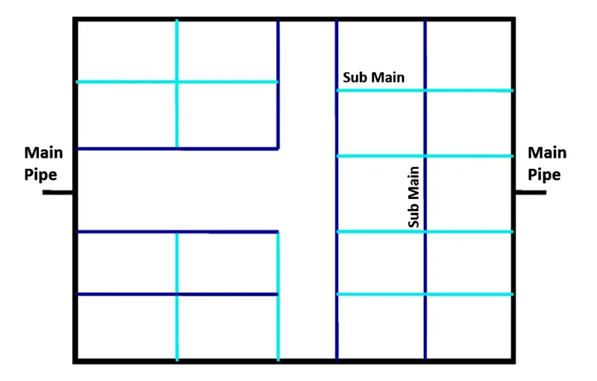
\includegraphics[scale=0.5]{RingDistributionSystem}}    
     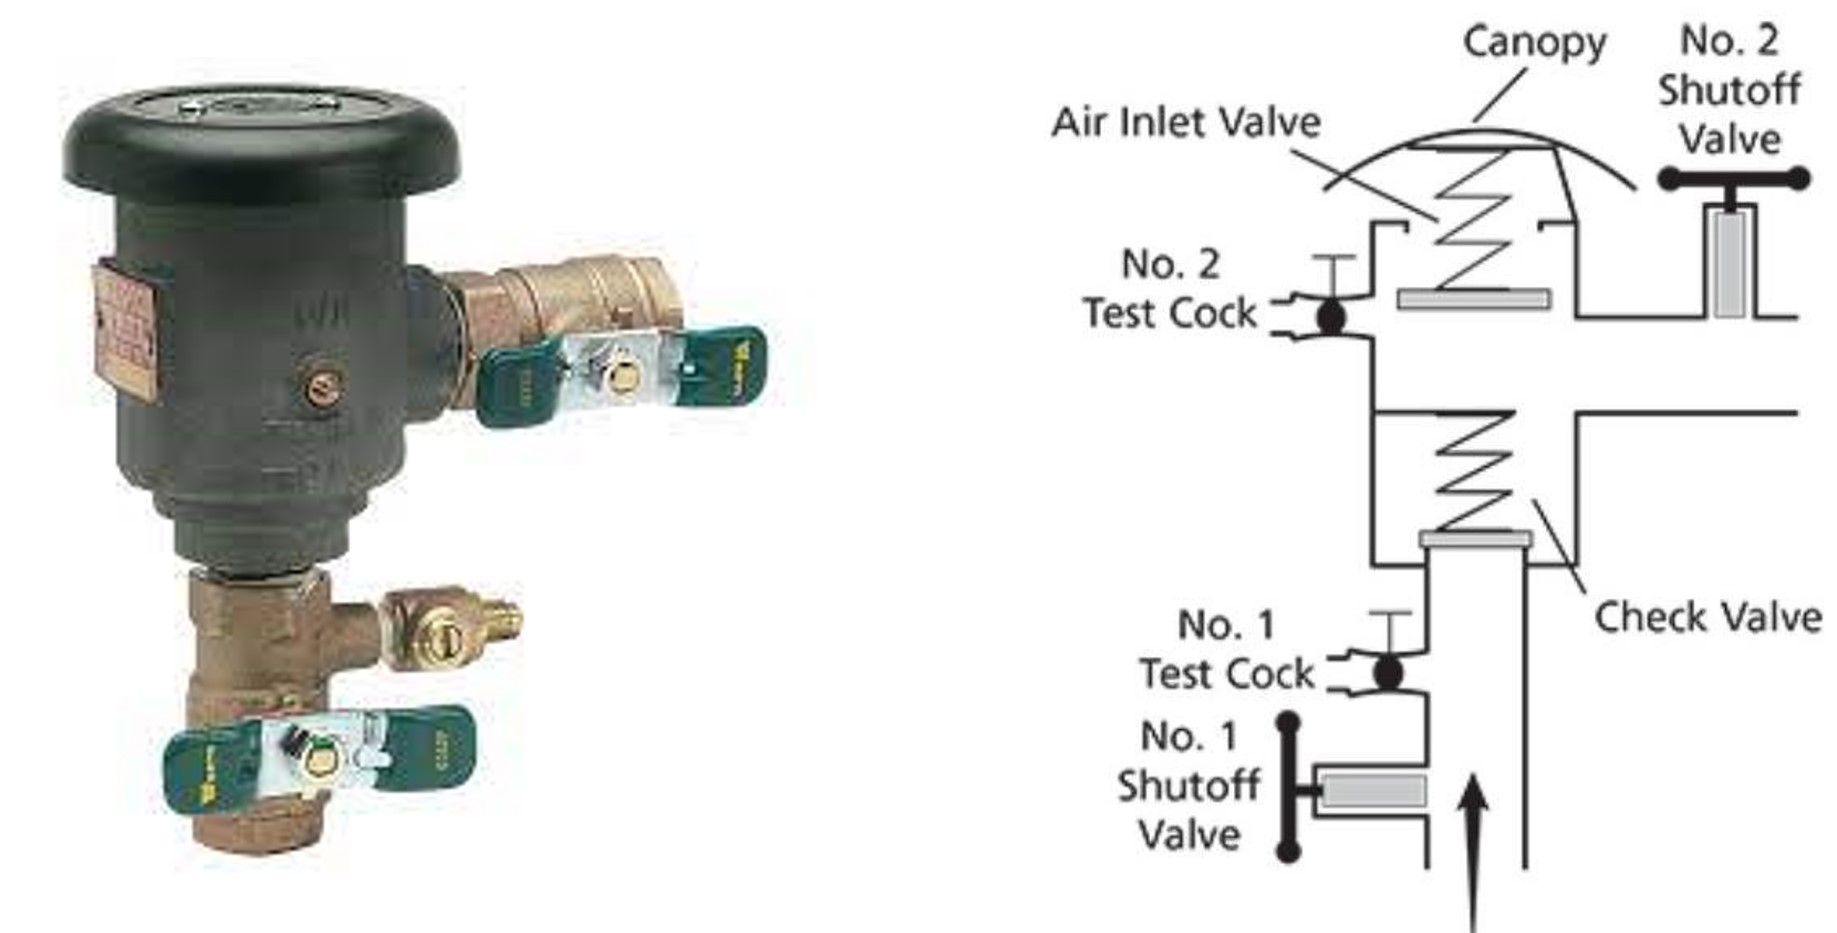
\includegraphics[scale=0.38]{SpillResitantVacuumBreaker1}\\
    \end{minipage}
     &
    \vspace{0.4cm}
    %\begin{minipage}[t]{5cm}
 \scriptsize{\begin{itemize}[topsep=5pt, partopsep=0pt]
\item Its assembly consists of an independently operating internally loaded check valve and independently operating loaded air inlet valve located on the discharge side of the check valve. 
\item The assembly is to be equipped with a properly located resilient seated test cock, a properly located bleed/vent port, and tightly closing resilient seated shutoff valves attached at each end of the assembly. 
\item This assembly is designed to protect against a non-health hazard(i.e., pollutant) or a health hazard (i.e., contaminant) under a backsiphonage condition only.

\textbf{Common Applications - Irrigation systems}
\end{itemize}}
\\ \hline

\multicolumn{2}{c}{Swing Check Valve} \index{Backflow!Prevention devices!Swing check valve}\\ \hline
    \begin{minipage}{.3\textwidth}
%    \tcbox[colframe=green!30!black,
%           colback=green!30]{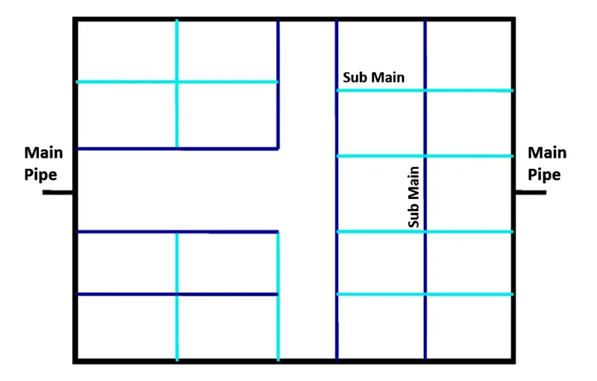
\includegraphics[scale=0.5]{RingDistributionSystem}}    
     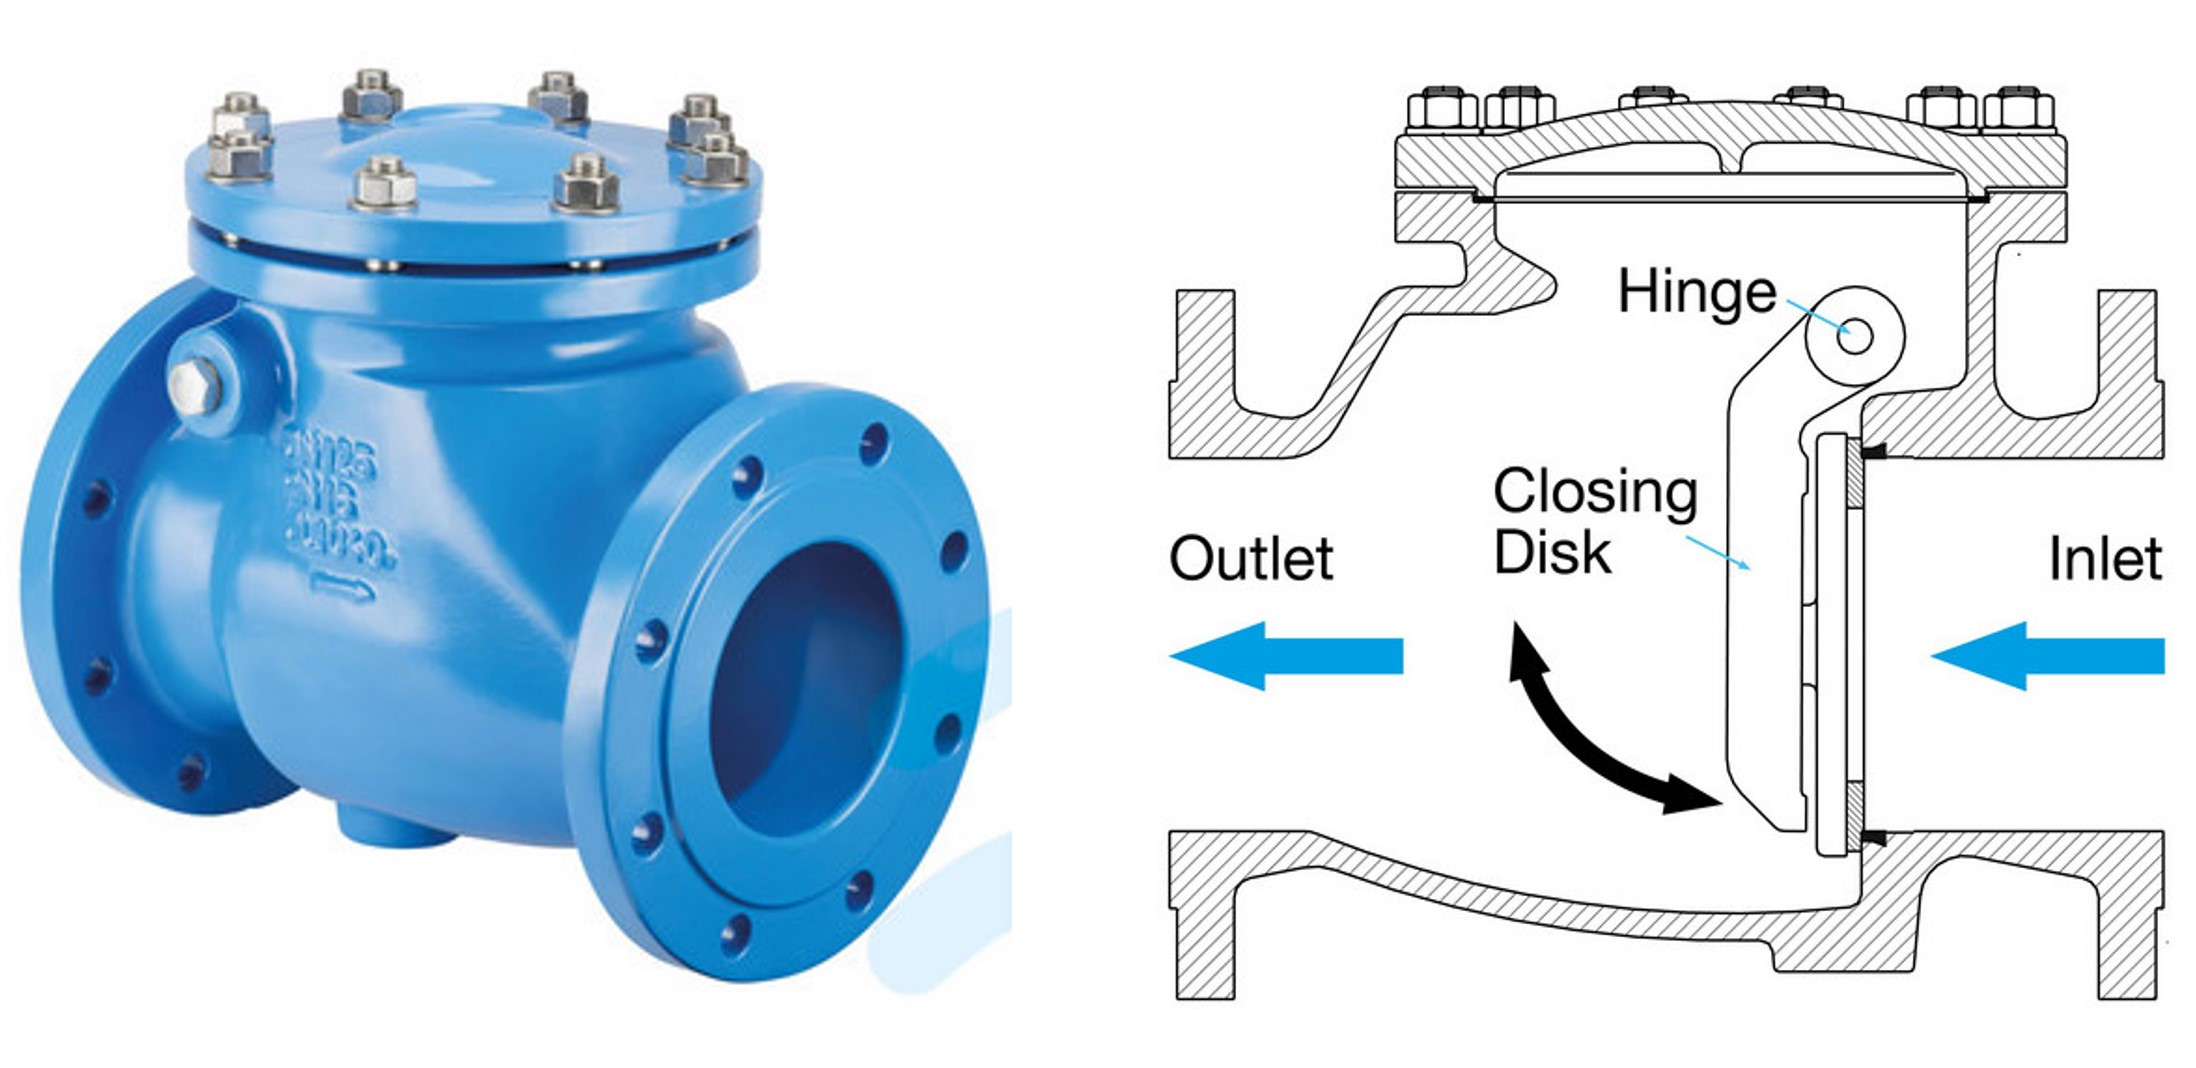
\includegraphics[scale=0.3]{SwingCheckValve1}\\
    \end{minipage}
     &
    \vspace{0.4cm}
    %\begin{minipage}[t]{5cm}
 \scriptsize{\begin{itemize}[topsep=5pt, partopsep=0pt]
\item The swing check valve consists of a valve body, seat, and disc linked to the hinge. 
\item Upon encountering a specified flow rate, the disc rotates to a horizontal position, enabling forward flow. It returns to the valve seat when the flow stops to prevent backflow. 
\item It provides a simple way to prevent backflow due to back pressure.

\textbf{Common Applications - Pumping systems}
\end{itemize}}
\\ \hline
    %\end{minipage}
\end{tabular}
\caption{Backflow prevention devices - Table 1 of 2}  
                \label{table:Backflow1} 
\end{table}
\vspace{-2em}

\end{landscape}

\thispagestyle{empty}
\begin{landscape}





\begin{table}[h!]
  \begin{tabular}{|c m{20cm} |}
    \hline
\multicolumn{2}{c}{Double Check Valve Assembly} \index{Backflow!Prevention devices!Double check valve assembly}\\ \hline
    \begin{minipage}{.3\textwidth}
    \hspace{1cm}
%    \tcbox[colframe=green!30!black,
%           colback=green!30]{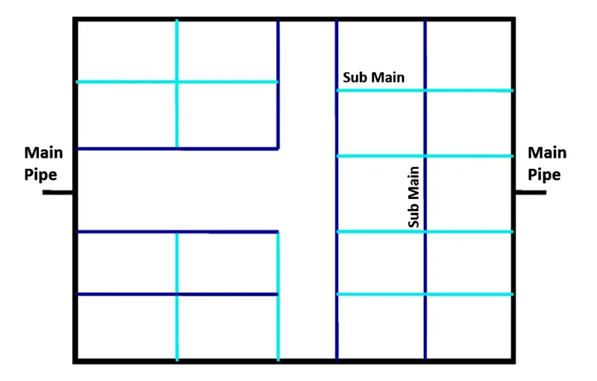
\includegraphics[scale=0.5]{RingDistributionSystem}}    
     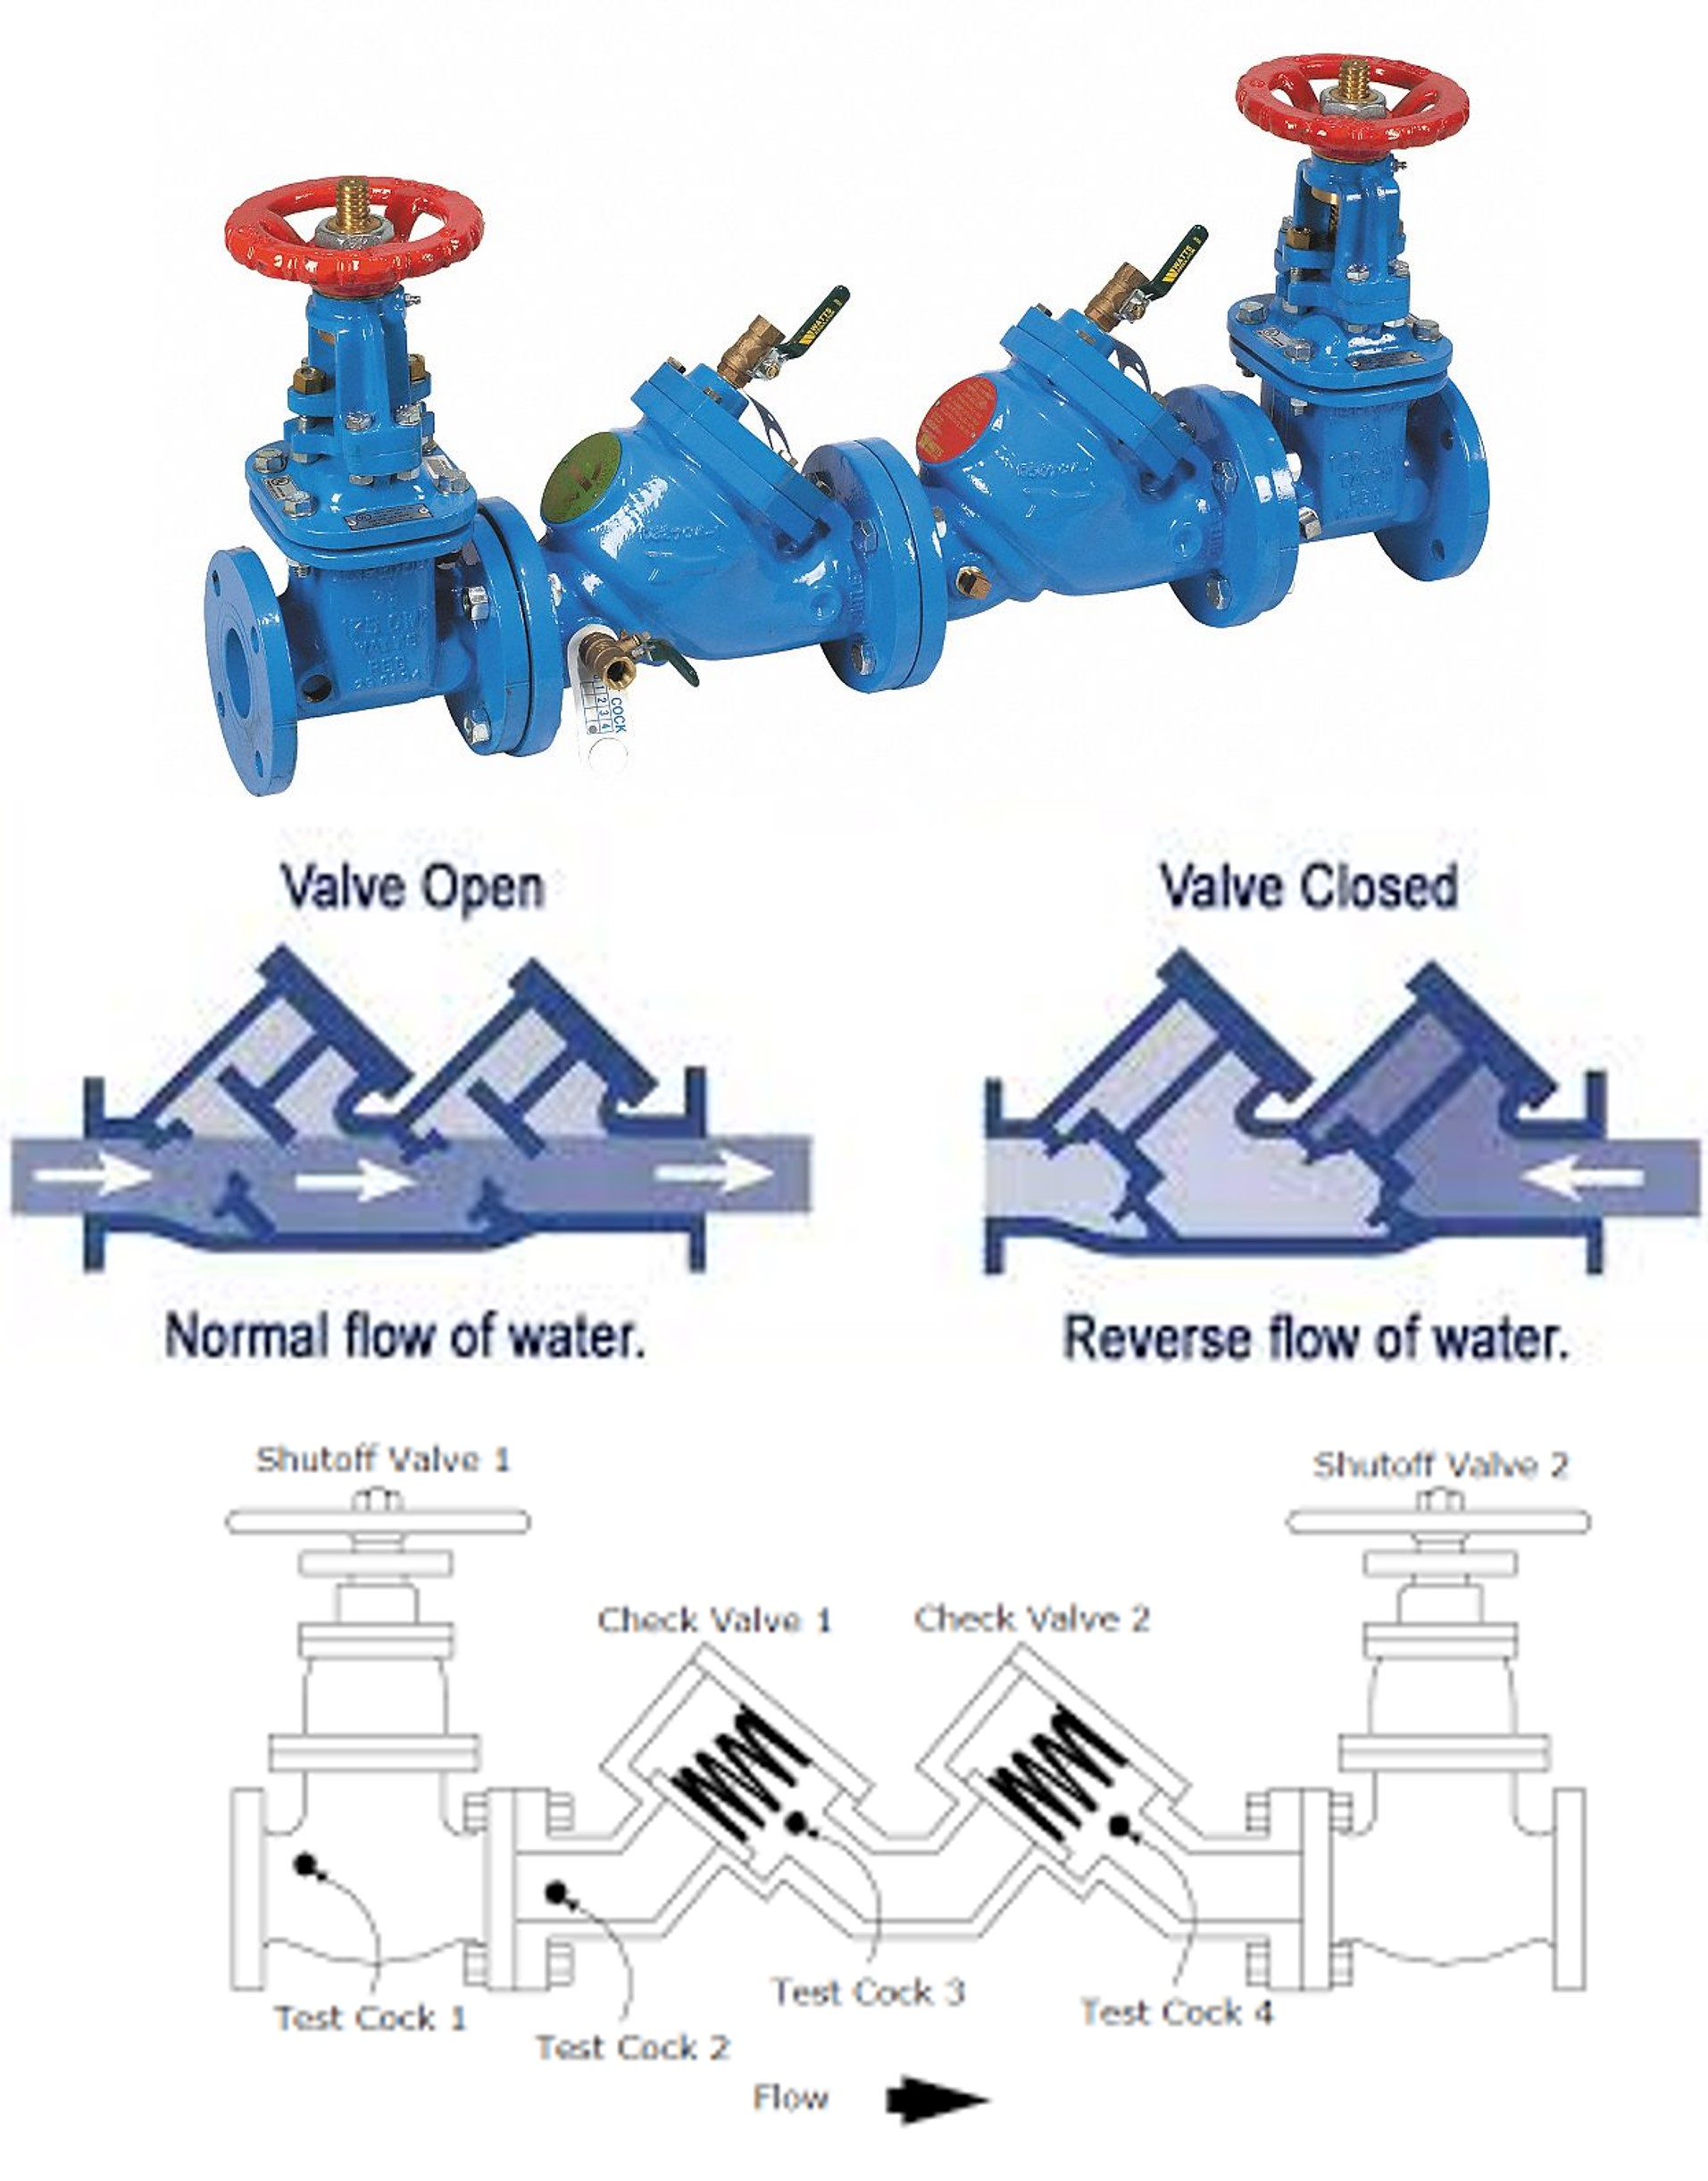
\includegraphics[scale=0.35]{DoubleCheckValve1}\\
    \end{minipage}
     &
    \vspace{0.8cm}
    %\begin{minipage}[t]{5cm}
\scriptsize{\begin{itemize}[topsep=5pt, partopsep=0pt]
\item Its assembly is composed of two independently acting, approved check valves, including tightly closing resilient seated shutoff valves attached at each end of the assembly and fitted with properly located resilient seated test cocks.
\item This assembly is used to protect against a non-health hazard (i.e., pollutant)

\textbf{Common Applications - Fire sprinkler systems, non-hazardous irrigation, combi-boilers, non-health hazards}

\end{itemize}}
\\ \hline

\multicolumn{2}{c}{Reduced Pressure Zone Assembly} \index{Backflow!Prevention devices!Reduced pressure zone (RPZ)}\\ \hline
    \begin{minipage}{.3\textwidth}
    \hspace{0.3cm}
%    \tcbox[colframe=green!30!black,
%           colback=green!30]{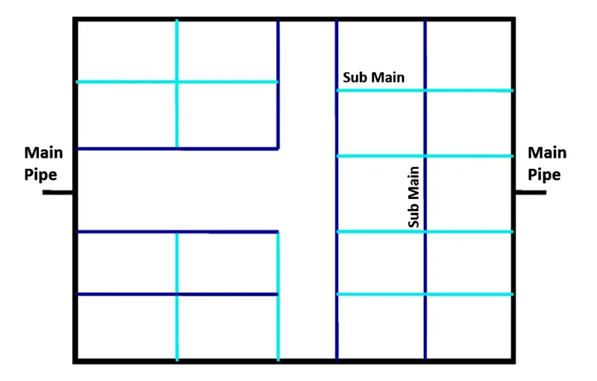
\includegraphics[scale=0.5]{RingDistributionSystem}}    
     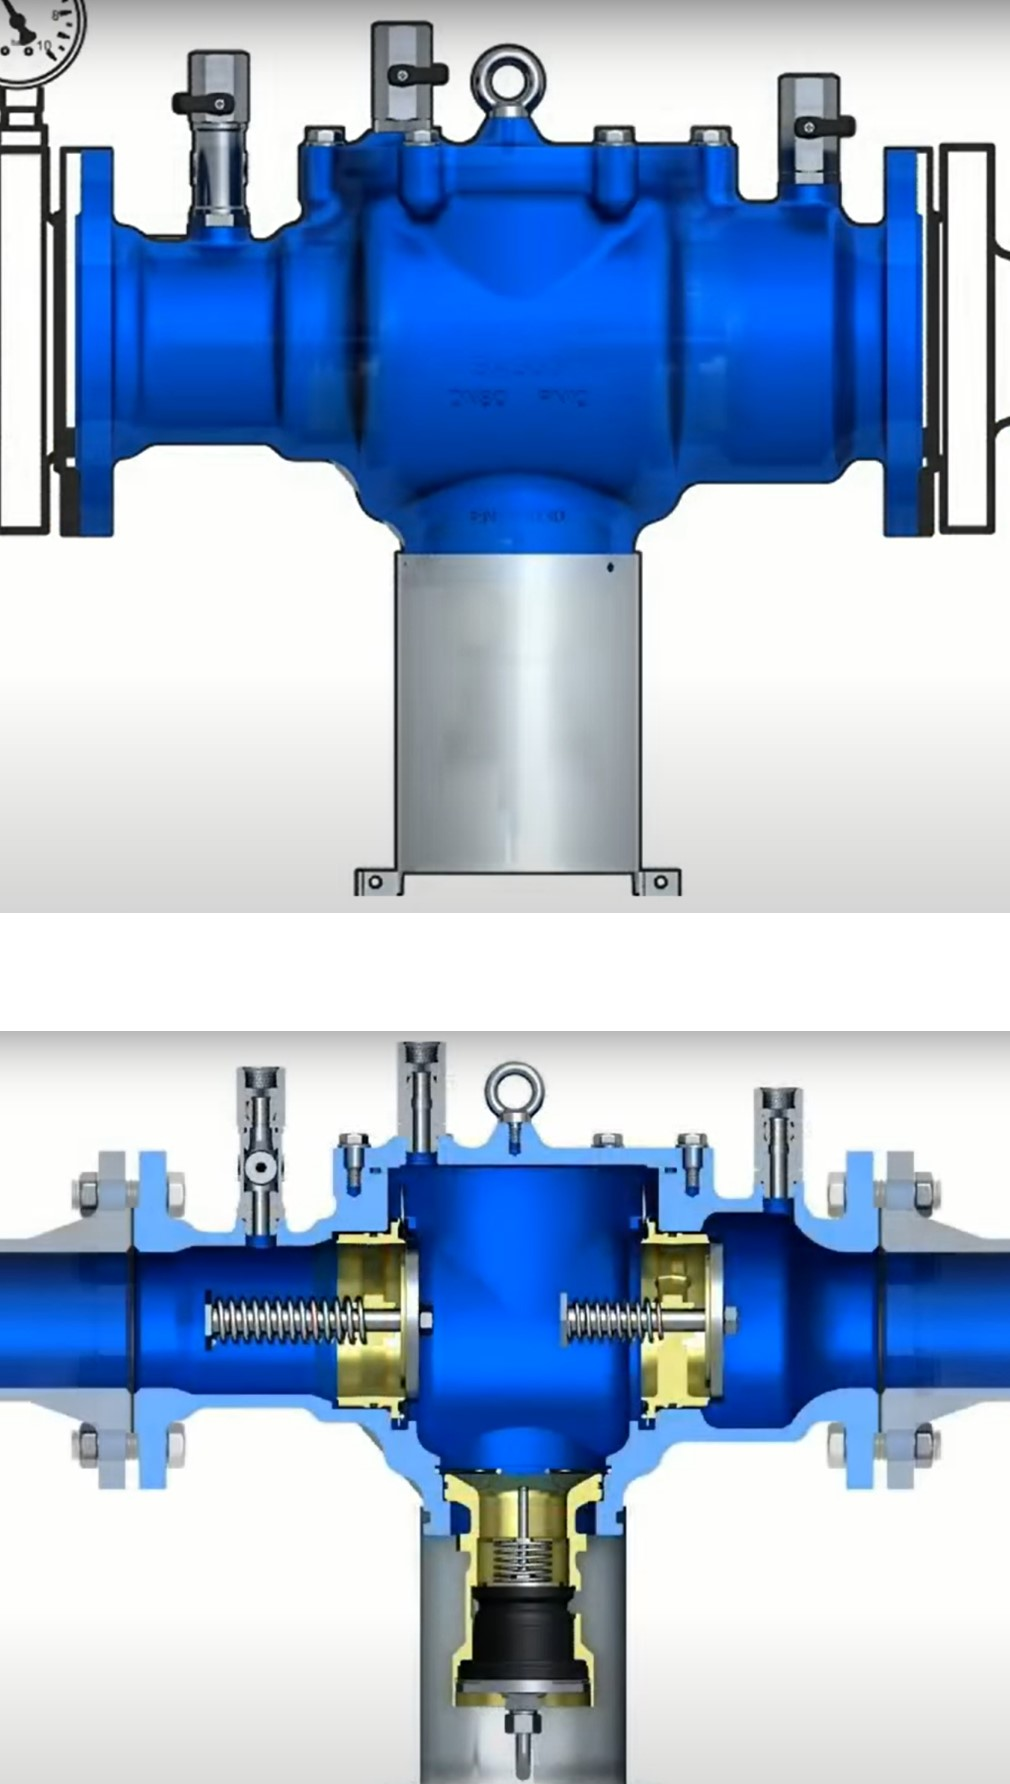
\includegraphics[scale=0.32]{ReducedPressurePrinciple1}\\
    \end{minipage}
     &
    \vspace{0.8cm}
    %\begin{minipage}[t]{5cm}
\scriptsize{\begin{itemize}[topsep=5pt, partopsep=0pt]
\item This assembly includes two independently acting check valves and an intermediate relief valve that opens to the atmosphere if both check valves should fail. \item Also includes properly located resilient seated test cocks and tightly closing resilient seated shutoff valves at each end of the assembly.

\item This is considered suitable for significant hazard applications that is, where the consequence of backflow into the water supply would cause significant harm.
\item They are considered suitable because they prevent both back pressure and back-siphonage, 
\item Its redundant design allows it to provide protection even with two check valves broken
\item  This assembly is not for backflow protection of sewage or reclaimed water.

\textbf{Common Applications – Domestic water and irrigation service protection, health hazards}
\end{itemize}}
\\ \hline
    %\end{minipage}
\end{tabular}
\caption{Backflow prevention devices - Table 2 of 2}  
                \label{table:Backflow2} 
\end{table}

\end{landscape}

\section{Fire Hydrants}\index{Fire hydrants}
\begin{itemize}
\item Fire hydrants is a visible connection pint in the water distribution system to provide water at a high flow rates primarily for:
\begin{itemize}
\item Fire fighting
\item  Flushing distribution systems
\item For other utilities, such as street cleaning and sewer cleaning
\end{itemize}
\item Hydrants can be categorized as:
\begin{itemize}
\item Wet barrel \index{Fire hydrants!Wet barrel}
\begin{itemize}
\item Have the operating valve in the nozzle section
of the hydrant and are operated by rotating the operating stem on each of the outlets.
\item These hydrants are used in warm climates where it rarely freezes.
\item Their main advantage is the ease of connecting a second fire truck. 
\item Each discharge port is independently valved.
\end{itemize}
\item Dry barrel \index{Fire hydrants!Dry barrel}
\begin{itemize}
\item These have the operating valve installed below
ground.
\item The hydrant is equipped with a special drain valve that allows the above ground portion to automatically drain when not in use. 
\item The dry barrel
hydrant is widely used in colder climates. 
\item Its main advantage is that it is less
likely to freeze and normally not loose water when hit by a vehicle.
\item The dry-barrel hydrant must always be opened completely and never partially as the partially opened hydrant will allow pressurized flow through the drain valve, which may wash away the soil from the area surrounding the base, or the partially open main valve may trap small stones or other debris between the valve seal and seat.
\end{itemize}
\item A flush hydrant sits flush with the
surface of the ground and is used in airports, on bridges, and other places where the exposure of the hydrants is more of a hazard than the difficulty of connecting to a ground-level hydrant. 
\end{itemize}
\newpage
\end{itemize}
\begin{table}[H]
\begin{center}
        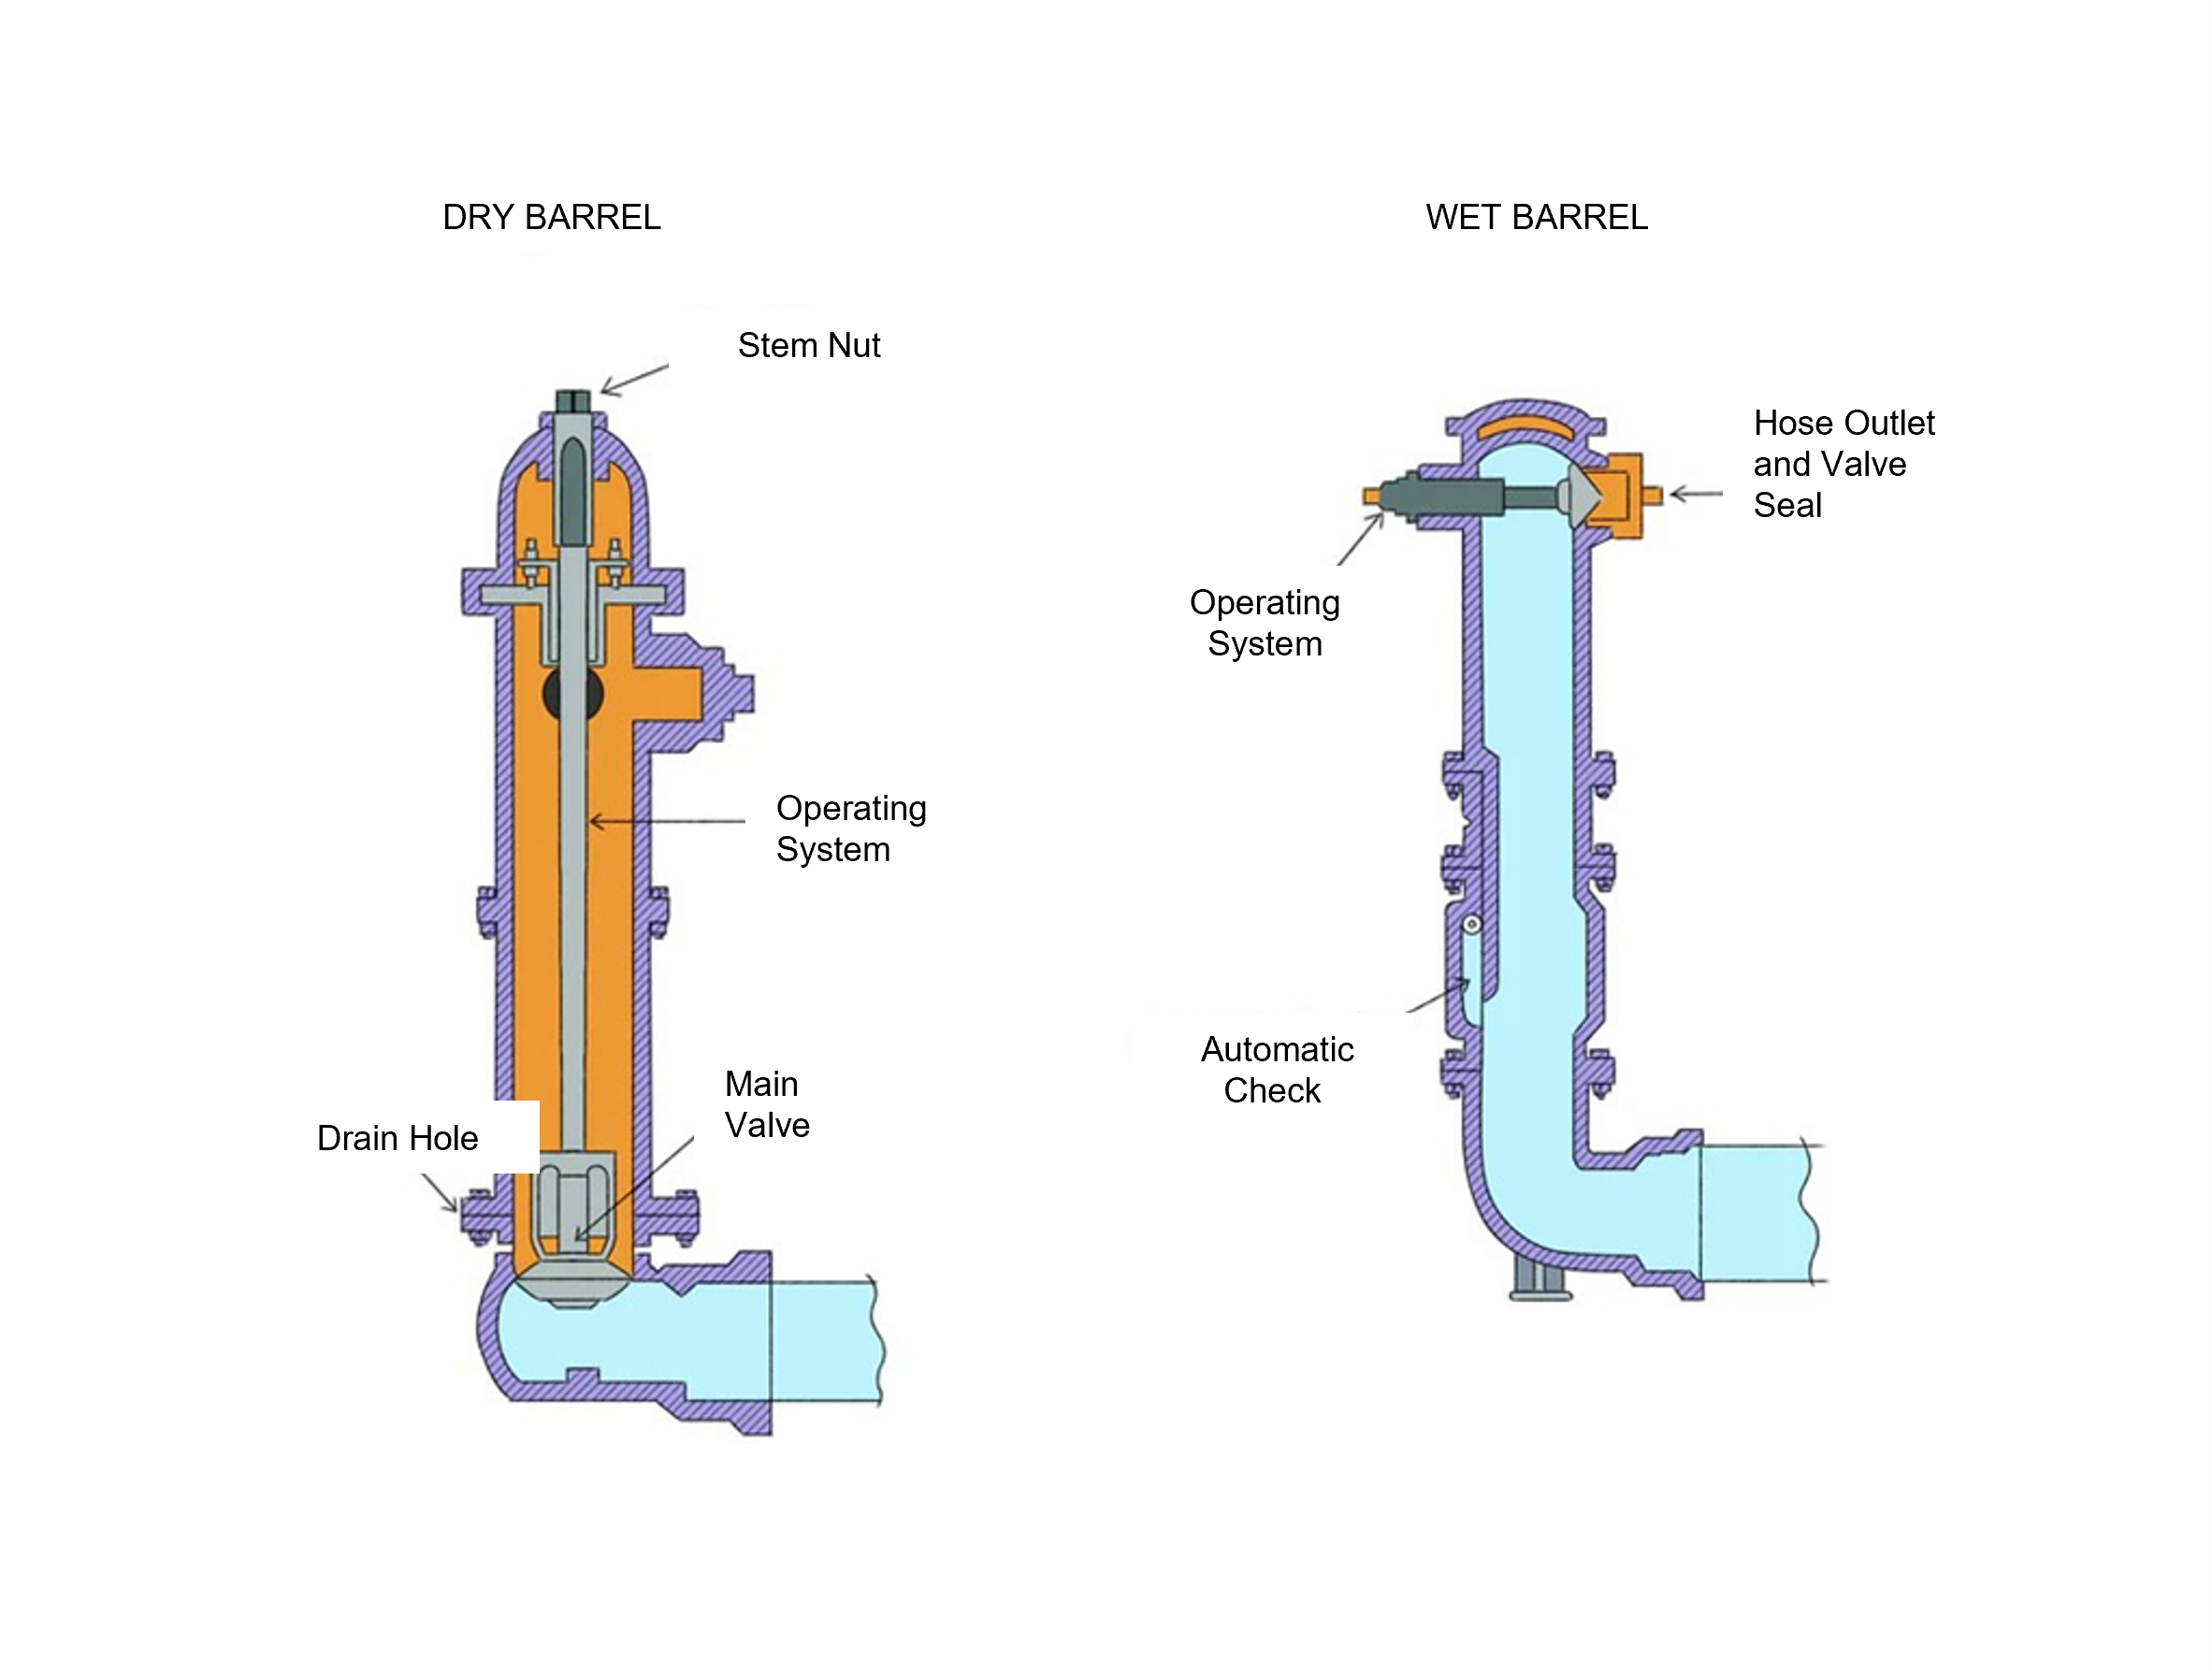
\includegraphics[scale=0.85]{FireHydrantTypes2}
        \caption{Types of fire hydrants}
\end{center}
\end{table}

\section{Water Meters}\index{Water meters}
\begin{itemize}
\item \begin{singlespacing}Meters measure, display, and record the amount of water that passes through a distribution system component. \end{singlespacing}

\item Typical applications of meters in a distribution network include:

\begin{itemize}
\item Measuring the amount of water supplied to the system.

\item Measuring the amount of water supplied to a particular area of the system, including through a pump station or control valve.

\item Measuring the amount of water used by a customer, for billing purposes.

\item Monitoring unaccounted-for water in a distribution network.\\

\end{itemize}
\item Table ~\ref{table:Watermeters} summarizes the properties and use of the commonly used distribution system water meters.
\end{itemize}
\vspace{-0.5em}
\newpage

\begin{table}[h!]
  \centering
  \begin{tabular}{|c m{11cm} |}
    \hline
\multicolumn{2}{c}{Positive Displacement (PD) Meter} \index{Water meters!Positive displacement or nutating disc type}\\ \hline
    \begin{minipage}{.25\textwidth}
    \hspace{1cm}
%    \tcbox[colframe=green!30!black,
%           colback=green!30]{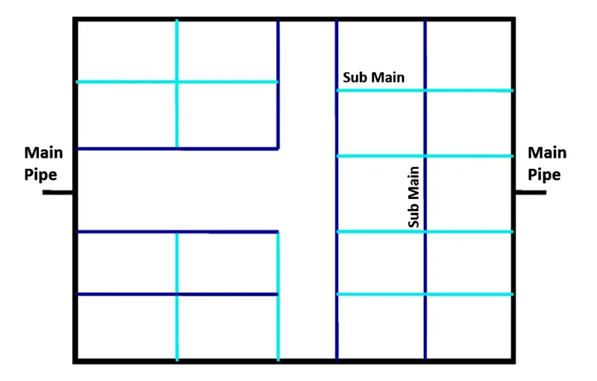
\includegraphics[scale=0.5]{RingDistributionSystem}}    
     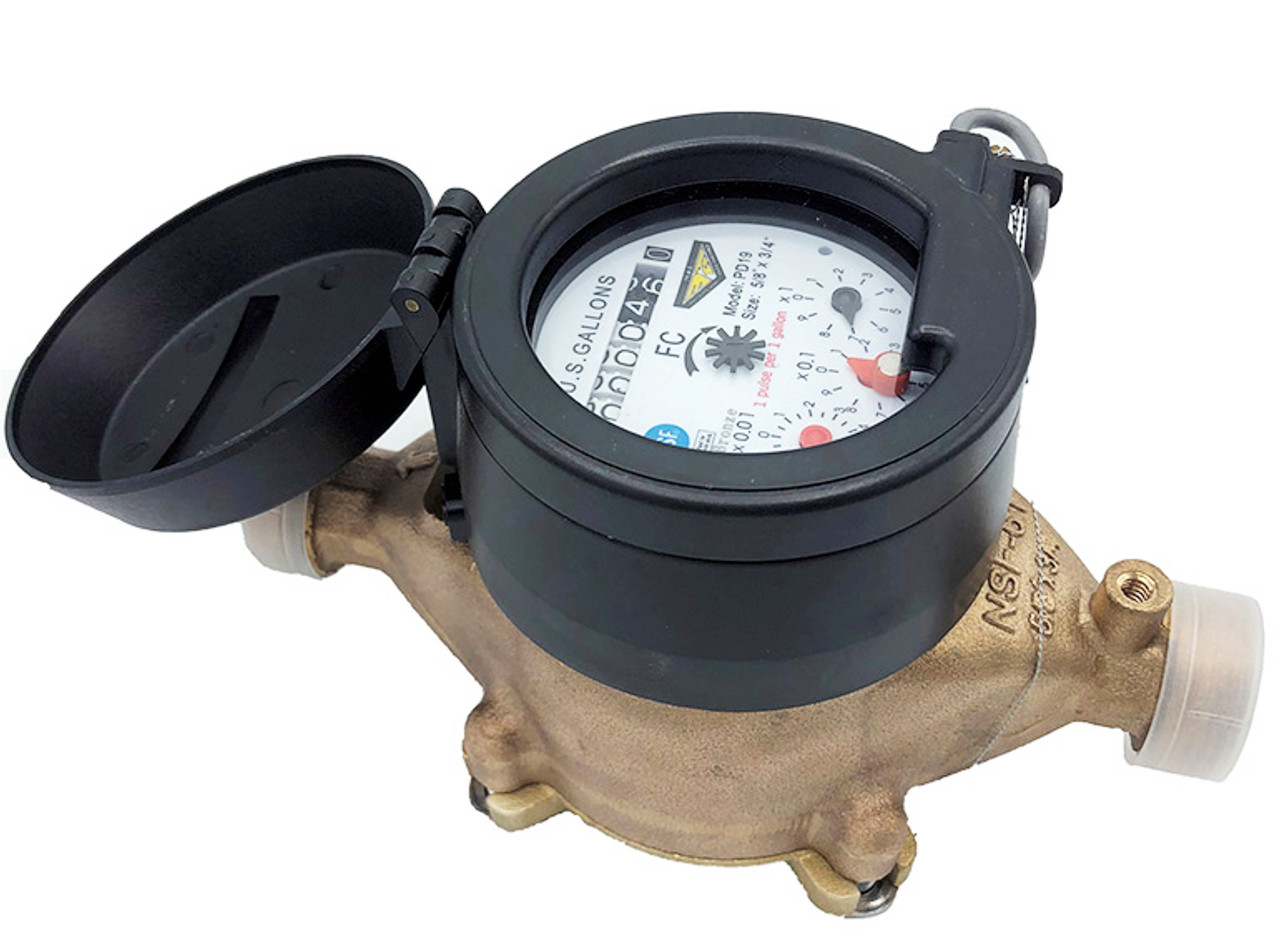
\includegraphics[scale=0.08]{PDMeter}
\\
    \end{minipage}
     &
    \vspace{0.3cm}
    %\begin{minipage}[t]{5cm}
      \begin{itemize}[leftmargin=*]

  \item Nutating disc flow meter is the most common types of PD flow meter. A disc mounted to a central ball wobbles (nutates) when fluid enters the chamber, transferring the displaced volume to the register.
  
  \item Commonly used as customer service meters.

  \item Typically has a diameter of 2-inches or less.

  \item Generally used to measure low flow rates.

  \item Have limitations at very high flows.

\end{itemize}
\\ \hline

\multicolumn{2}{c}{Velocity Meter} \index{Water meters!Velocity meter}\\ \hline
    \begin{minipage}{.25\textwidth}
%    \tcbox[colframe=green!30!black,
%           colback=green!30]{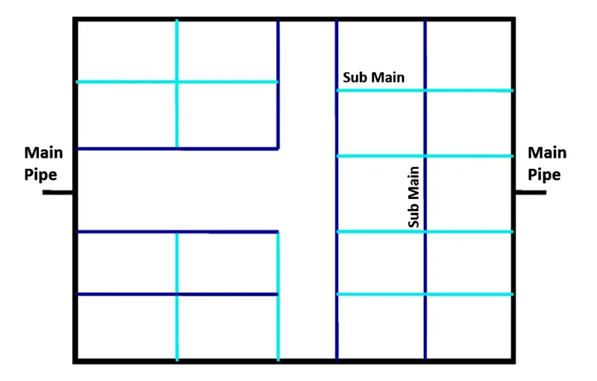
\includegraphics[scale=0.5]{RingDistributionSystem}}    
     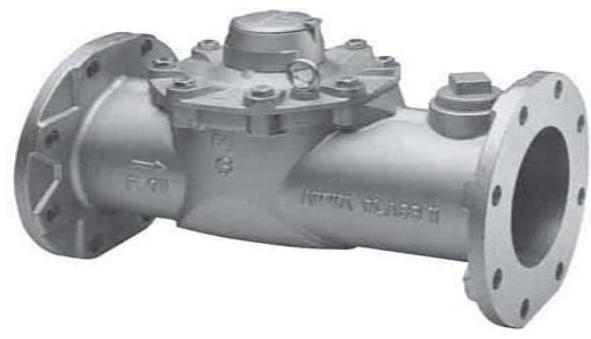
\includegraphics[scale=0.15]{VelocityMeter}\\
    \end{minipage}
     &
    \vspace{0.3cm}
    %\begin{minipage}[t]{5cm}
      \begin{itemize}[leftmargin=*]

\item Commonly used in pump stations, industrial facilities, and large diameter mains to measure high rates of flow.

  \item Does not accurately measure low flow rates.

  \item Includes the Venturi, Turbine, and Propeller type meters.


\end{itemize}
    %\end{minipage}
    
    \\ \hline

\multicolumn{2}{c}{Compound Meter}\index{Water meters!Compound meter}\\ \hline
    \begin{minipage}{.25\textwidth}
%    \tcbox[colframe=green!30!black,
%           colback=green!30]{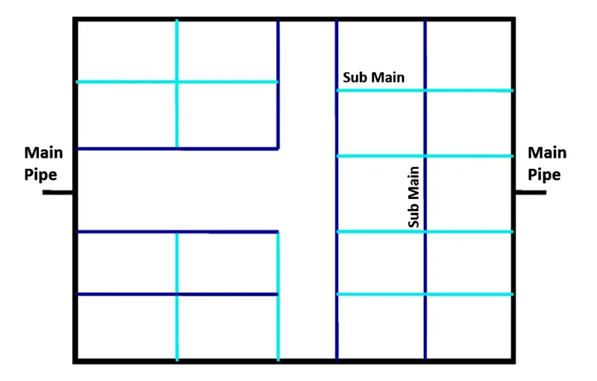
\includegraphics[scale=0.5]{RingDistributionSystem}}    
     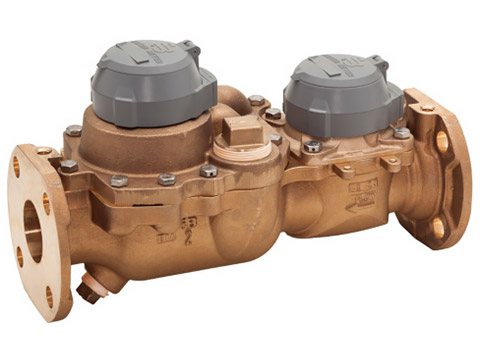
\includegraphics[scale=0.16]{CompoundMeter}\\
    \end{minipage}
     &
    \vspace{0.4cm}
    %\begin{minipage}[t]{5cm}
      \begin{itemize}[leftmargin=*]

  \item Commonly used to measure flow at apartment complexes, schools, and industries that can typically have high peaks in water use compared with daily averages.

  \item Composite of the displacement and velocity meters.

  \item Used to measure flowrates that vary widely.


\end{itemize}
\\ \hline
    %\end{minipage}

\multicolumn{2}{c}{Electronic Meter}  \index{Water meters!Electronic meter}\\ \hline
    \begin{minipage}{.25\textwidth}
    \hspace{1cm}
%    \tcbox[colframe=green!30!black,
%           colback=green!30]{\includegraphics[scale=0.5]{RingDistributionSystem}}    
     \includegraphics[scale=0.13]{ElectronicMeter}\\
    \end{minipage}
     &
    \vspace{0.8cm}
    %\begin{minipage}[t]{5cm}
      \begin{itemize}[leftmargin=*]



  \item Measures flow magnetically (mag meter) \index{Water meters!Electronic meter!Mag-meter}or sonically.

  \item Highly accurate if properly located.


\end{itemize}
\\ \hline

\multicolumn{2}{c}{Proportional Meter}\\ \hline
    \begin{minipage}{.25\textwidth}
%    \tcbox[colframe=green!30!black,
%           colback=green!30]{\includegraphics[scale=0.5]{RingDistributionSystem}}    
     \includegraphics[scale=0.35]{ProportionalMeter}\\
    \end{minipage}
     &
    \vspace{0.8cm}
    %\begin{minipage}[t]{5cm}
      \begin{itemize}[leftmargin=*]

  \item Measures high flowrates at larger pipes such as fire service lines.
  \item It has a small bypass meter, located parallel to the main pipe which is calibrated to measure the flow through the main pipe.
  \item Does not measure low flows accurately.


\end{itemize}
\\ \hline
    %\end{minipage}
\end{tabular}
\caption{Types of water meters}  
                \label{table:Watermeters} 
\end{table}


\vspace{-2em} 

\section{Distribution System Operation and Maintenance Elements}\index{Distribution system operation and maintenance elements}


\subsection{Maintaining distribution system pressure} \index{Maintaining distribution system pressure}
\begin{itemize}
\item Distribution systems must be maintained under pressure at all times to help ensure that contamination does not enter the system. 
\item In the event that the distribution system is de-pressurized, the water system operator must promptly restore pressure and take corrective action to monitor and restore water quality.  The corrective action should include flushing and disinfection.
\end{itemize}

\subsection{System Disinfection Program} \index{Disinfection!System disinfection program}
\subsubsection{Disinfecting new and existing wells} \index{Disinfection!Disinfecting new and existing wells}
Well disinfection under the following circumstances should be performed in accordance with the American Water Works Association C654-03 \index{Disinfection!AWWA Standard!C654-03 Disinfection of wells}, and re-sampled for bacteriological quality and the test results shall be submitted to the State Board for review and approval before the well is placed into service: \\
\begin{itemize}
\item A new or repaired well, or a well that has not been in operation for more than three months
\item When coliform bacteria are present in the water
\item After flooding of the well
\item After plumbing installation, e.g. softeners, sinks, filters
\item After casing or pump repairs - submersible types or other
\item When water taste or odor changes, e.g. from iron or sulfur reducing bacteria
\item As part of annual maintenance
\item During startup of seasonal wells
\item Elements of well disinfection include:
\begin{itemize}
\item Disinfection is accomplished using sodium hypochlorite
\item A 50 mg/l chlorine concentration is recommended with a 24-hour contact time
\item Application of bleach through the pump column pipe is preferred over the application using the vent pipe as the chlorine injection point.
\item At the end of the disinfection period, the well is pumped until all evidence of residual is gone.
\end{itemize}
\end{itemize}

\subsubsection{Disinfecting Water Mains} \index{Disinfection!Disinfecting water mains}
\begin{itemize}
\item Disinfection of repaired mains is not required, if the repairs are done with the line full of water and under pressure.
\item Utmost care should be taken to prevent contamination during installation or repairs
\item Valves and fittings must be cleaned during installation. 
\item Sections of pipes, fittings and valves and other items that will not be disinfected by the filled line must be precleaned and disinfected. 
\item Prior to use, newly installed water mains, or water mains that have been taken out of service for maintenance or repair, shall be disinfected and sampled for bacteriological quality in accordance with American Water Works Association Standard C651-05 \index{Disinfection!AWWA Standard!C651-05 Disinfection of water mains}.
\item Crushed HTH tablets be placed in joints and hydrant branches to improve disinfection of spaces that are difficult to chlorinate once filled with water.
\
\item Flushing the mains for atleast 30 minutes at a minimum velocity of 2.5 ft/sec is recommended prior to disinfection
\item Common methods for disinfecting water mains are:\\
\vspace{0.3cm}
\begin{tabular}{ | p {3 cm} | m {3 cm}| m{3 cm} | m{3 cm} |} 
 \hline
\thead{METHOD}&\thead{MAX. CHLORINE\\DOSAGE (mg/l)}&\thead{MINIMUM CONTACT\\TIME (hr)}&\thead{MINIMUM CHLORINE\\RESIDUAL (mg/l)}  \\ 
 \hline
 Continuous & \multicolumn{1}{c|}{50} & \multicolumn{1}{c|}{24} & \multicolumn{1}{c|}{25} \\
 \hline
  Slug & \multicolumn{1}{c|}{500} & \multicolumn{1}{c|}{3} & \multicolumn{1}{c|}{300} \\
 \hline
  Tablet & \multicolumn{1}{c|}{50} & \multicolumn{1}{c|}{24} & \multicolumn{1}{c|}{25} \\
 \hline
\end{tabular}\\
\vspace{0.3cm}
\item Post-disinfection, lines must be flushed until chlorine residual is less than 1 mg/l
\item Bacteriological test - 24-hour membrane filter test is required to be conducted after disinfection and prior to placing the line in service.
\end{itemize}

\subsubsection{Disinfecting Water Storage Tanks} \index{Disinfection!Disinfecting water storage tanks}
\begin{itemize}
\item After the repair/rehabilitation of the water tank is conducted or after the construction of the new tank, prior ot putting the tank in-service, the surfaces of the walls, floor, and operating facilities of the storage facility shall be cleaned thoroughly by use of a high pressure water jet, sweeping, scrubbing, or equally effective means. 

\item After the cleaning, the tank is required to be disinfected and is deemed adequately disinfected and ready for service only if the bacteriological testing results show negative coliform results.

\item AWWA C652-19 \index{Disinfection!AWWA Standard!C652-19 Disinfection of water storage facility} Disinfection of Water Storage Facility is the standard for disinfection of water-storage facilities describes materials, facility preparation, application of disinfectant to interior surfaces of facilities, and sampling and testing for the presence of coliform bacteria, chlorine residual, and acceptable aesthetic water quality. 

\item Acceptable water storage disinfection procedures include:
\begin{enumerate}
\item A new tank can be disinfected by filling the tank to the overflow level with potable water with an initial chlorine concentration of 50 mg/L in the full tank and holding that water for 24 hours.

\item Application of a chlorine solution containing at least 200 mg/L of free available chlorine using either spray equipment or brushes followed by keeping the chlorine solution in contact with the tank surfaces for at least 30 minutes.  The tank is then filled with the distribution system water that is treated with chlorine to provide a residual of atleast 3 mg/l and held for 3-6 hours.  
\end{enumerate}
\item After the disinfection step is completed, the tank is filled with potable water to the overflow level and tested for satisfactory bacteriological quality before placing the tank in service.

\item For the bacteriological testing, two water samples from the tank are to be collected at least 24 hours apart and analyzed by a certified laboratory. The results of these samples must indicate no coliform contamination before the pipe, tanks, or equipment can be utilized as part of the water distribution system. 
\end{itemize}

\subsection{Controlling nitrification} \index{Nitrification!Control in distribution system}
\begin{itemize}
\item Nitrification is a microbial process that converts ammonia and similar nitrogen compounds into nitrite (NO$_2$) and then nitrate (NO$_3$).
\item Nitrification may particularly be an issue in water systems where ammonia is added to form chloramines.
\item The problem is greatest when temperatures are warm and water usage is low.
\item Nitrification control measures include:
\begin{itemize}
\item Optimizing the chloramination process.
\item Reducing the water age by flushing routinely and deep cycling storage tanks.
\item Hard flushing or mechanically pigging the distribution system, and conducting valve maintenance.
\item Replacing aging infrastructure as tuberculation in older pipes would allow biofilm accumulation.
\item Managing disinfectants in source waters containing chlorine and other sources that contain chloramines by blending.
\item Regular monitoring of the system for nitrification.
\end{itemize}
\end{itemize}



\subsection{System Flushing Program} \index{System flushing program}
\begin{itemize}
\item Each public water system should flush the water distribution system as necessary to reduce stagnant water and sediment build-up.
\item Biofilm or slime growth along with sediment deposits in the distribution pipes increases the chlorine demand and also negatively affect the water quality.
\item Flushing improves the water quality and also the carrying capacity of the pipes.
\item Flushing is normally practiced after receiving water quality complaints or preemptively during spring to prevent the rapid growth of biofilm during summer.
\item Advance planning elements include: minimizing inconvenience to customers and traffic impacts, public notifications, identifying sections of mains to be flushed and required valving and resource allocations.
\item Unidirectional flushing - where the flushing start point is at or near the source of supply and working outward into the distribution system is usually practiced.
\item A minimum flushing velocity of 2.5 ft/sec is recommended.
\item Hydrants are opened for atleast 5 to 10 minutes to stir up deposits.
\item Usually lines are flushed for atleast 30 minutes while ensuring the system pressure of the affected area does not drop below 20 psi.
\item Water samples may be taken at the beginning ad after flushing to determine its effectiveness and to identify need for additional flushing.
\end{itemize}

\subsection{Valves Operation and Maintenance} \index{Valves operation and maintenance}
\begin{itemize}
\item Hydraulic problems associated with improper operation of valves include:
\begin{enumerate}
\item Cavitation \index{Cavitation}
\begin{itemize}
\item Cavitation is a common occurrence in valves used in throttling or modulating service during the last few degrees of closure when the supply pressure is greater than about 100 psig. 
\item Cavitation is the sudden vaporization and violent condensation of a liquid downstream of the valve due to localized low pressure zones. 
\item When flow passes through a throttled valve, a localized low pressure zone forms immediately downstream of the valve. If the localized pressure falls below the vapor pressure of the fluid, the liquid vaporizes (boils) and forms a vapor pocket. As the vapor bubbles flow downstream, the pressure
recovers, and the bubbles violently implode causing a popping or rumbling sound similar to tumbling rocks in a pipe. 
\item The sound of cavitation in a pipeline is unmistakable. 
\item Cavitation can quickly destroy valve internals and even erode through pipe walls.
\item The condensation of the bubbles not only produces a ringing sound, but also creates localized stresses in the pipe walls and valve body that can cause severe pitting.
\item 
\item Cavitation may be prevented by ensuring selection of right size, type and location of the valve.
\begin{figure}[H]
\begin{center}
\includegraphics[scale=0.8]{CavitationinValves}
\caption{Valve cavitation}
\end{center}
\end{figure}
\end{itemize}
\item Water Hammer \index{Water hammer}
\begin{itemize}
\item Water hammer is the result of a pressure surge, or high-pressure shockwave that propagates through a piping system when a fluid in motion is forced to change direction or stop abruptly. 
\item This shockwave is typically characterized by a marked banging or knocking sound on the pipes immediately after a shutoff.
\item Water hammer can occur when an open valve suddenly closes, causing the water to slam into it, or when a pump suddenly shuts down and the flow reverses direction back to the pump. 
\item Since water is incompressible, the impact of the water results in a shock wave that propagates at the speed of sound between the valve and the next elbow in the piping system or within the column of water after the valve.
\item Water hammer, like cavitation, has the potential to cause catastrophic destruction to the distribution system piping.
\item Selecting the correct valve and lengthening the valve closure duration help mitigate water hammer occurrence.
\item Additionally, installation of air relief valves, air chambers - short segment of pipe with an an empty/air filled chamber that cushions shock waves, and water hammer arrestors - comprised of springs and air bladders which operate similarly to air chambers to reduce shock waves downstream of quick closing valves.
\end{itemize}
\end{enumerate}
\item Valves must be maintained in working order.  This necessitates that valves be “exercised” on a routine basis and visually inspected for leaks on a regular basis.
\item Valve information including the following should be readily available:
\begin{itemize}
\item System map showing valve locations and system isolation points
\item Information on valve sizing, direction to open the valve, number of turns, model type and installation date
\end{itemize}
\item Adequate inventory of valves and its replaceable parts need to be maintained to ensure availability .
\item Detailed records of valve inspections and maintenance activities including inspection logs and service requests must be maintained.
\end{itemize}

\subsection{Distribution System Map} \index{Distribution system map}
\begin{itemize}
\item Each water system should maintain an accurate map of the distribution system piping and valves. 
\item The map should be sufficiently detailed to enable maintenance personnel to promptly locate facilities for repair or operational purposes.
\item All valves and pipes are shown on the system's "as built" plans.  They are updated as repairs are made.  In addition, the fixed facilities and structures are shown on the map.
\item Comprehensive \index{Distribution system map!Comprehensive map} and plat maps are typically used.
\item A comprehensive map provides an overall view of the entire distribution system.
\item A plat map \index{Distribution system map!Plat map} shows property boundaries and includes roads and location of utilities such as gas lines, access by water and sewer lines, as well as the location of buildings and other infrastructure on the property.\index{Plat map}
\item A map scale which is distance on the map and distance on the ground (actual), allows for showing locations and distances accurately on a sheet of paper of convenient size. \index{Map scale}
\item A map scale is provided on the map as a fraction or a ratio-1/10,000 or 1:10,000. These "representative fraction" scales mean that one unit of measurement on the map 1 inch or 1 centimeter represents 10,000 of the same units on the ground.
\item The scale used will be dependent on the size of system and the size of the map.  A commonly used scale for maps used for utilities is 1:600 - 1-inch on the map represents 600 inches or 50 feet (600 feet * 12inches/1 feet) on the ground.
\end{itemize}

\subsection{Distribution System Record keeping} \index{Distribution system record-keeping}
The minimum record keeping requirements include:
\begin{itemize}
\item Date, time and cause of any system pressure loss.
\item Corrective action taken in response to system pressure loss.
\item Distribution system repairs and maintenance: date, location and reason for repairs.
\end{itemize}

\subsection{Water Usage Records} \index{Water usage records}
\begin{itemize}
\item Each public water system should have production meters and should maintain records on water usage throughout the year. These records are kept for future information.
\end{itemize}

\subsection{Storage Tank Maintenance} \index{Storage tank maintenance}
\begin{itemize}
\item Water storage tanks should be inspected on a regular basis to ensure that the structure is in satisfactory condition and properly secured. 
\item Records should be maintained of these inspections.  
\item Access hatches should be locked and all openings to the tank should be properly screened.  \item Roofs should not allow entry of contaminants.
\item The storage tank is visually inspected weekly.  A detailed inspection is done on the tank every four (4) months.  
\item Applying protective coating - painting/coating, the internal and external walls of the tank needs to be conducted periodically.
\item Several tank coating related considerations and precautions include: 
\begin{itemize}
\item Selecting the right paint - paints containing lead, PCBs, trichloroethylene etc. should be avoided.
\item  Ensuring appropriate surface preparation and adequate coatings drying times are provided.
\end{itemize}
\item Periodic, visual inspections and detailed cleaning and internal inspections are required. 

\item Records of the inspections are kept and any problems noted.
\end{itemize}

\subsection{Lead and Copper Sampling}\index{Sampling!Lead and copper sampling}
\begin{enumerate}
\item Samples are collected at customer's tap usually by the customer.
\item Sample needs to be a first draw sample - not allowing the water to run and NOT flushing out the service line.
\item Sample is collected early in the morning - no water to be used for a minimum of six hours before a sample is collected, no flushing and no opening a faucet.
\item Samples are not be be collected from unoccupied home where water has not been used for over 24 hours.
\item Action level for lead is 0.015 mg/L and copper is 1.30 mg/L
\item Action level means entailing either service line replacement program or changing water quality parameters, or adding chemicals such as polyphosphate to the water to reduce its corrosion potential.
\end{enumerate}


\subsection{Computer Based Controls and Monitoring} \index{Computer based controls and monitoring}
\begin{enumerate}
\item SCADA \index{SCADA}
\begin{itemize}
\item SCADA - Supervisory Control and Data Acquisition is a  useful and now widely used  computer based control system
\item Distribution system components and operational parameters including - pressures, flows, meters, pump speed, wetwell levels, valve positions etc. can be monitored and controlled onsite or from a central location using SCADA.
\item SCADA allows for monitoring system operations to identify excursions of operating equipment from normal operating conditions/ranges and help predict/identify maintenance, repair and replacement requirements.
\end{itemize}
\item Automated Meter Reading 
\begin{itemize}
\item  Automated Meter Reading (AMR) is the communication technology water utilities use to automatically collect water consumption and status data from water meters. 
\item After collection, the meter data is transferred to a database where utilities can monitor and analyze usage, troubleshoot issues and bill customers based on actual consumption, rather than predictions that were often required with bi-monthly or quarterly manual reads.
\end{itemize}
\item Advanced Metering Infrastructure 
\begin{itemize}
\item Advanced metering infrastructure (AMI) is an integrated system of water meters, communication networks and data management systems that enables two-way communication between meter endpoints and utilities.  
\item The utility can use the data to improve operational efficiencies and sustainability by effectively monitoring water usage and system efficiency, detecting malfunctions and recognizing irregularities.
\end{itemize}
\end{enumerate}

\subsection{Corrosion Control} \index{Corrosion control}
\begin{itemize}
\item Metallic elements of the water distribution system, including pipes and fittings, is subject to corrosion where the metal is converted to its salt or oxide.
\item Corrosion in the water distribution system leads to:

\begin{itemize}
\item Reduced mechanical strength leading to a loss in service life and piping failures - leaks and ruptures.
\item Leaching of toxic metals such as lead and copper into the drinking water
\item Formation and deposition of corrosion by-products in pipes made from material which include iron, leading to:

\begin{itemize}
\item Desposition of corrosion products on the inside surface of the pipe - \textbf{Tuberculation}  \index{Tuberculation} increase the roughness of the pipe, increasing the resistance to water thereby decreasing the water carrying capacity of the pipe and increasing the pumping cost.
\begin{figure}[h]
			      	\begin{center}
			      		\includegraphics[scale=0.07]{Tuberculation.jpg}\\
			      		\caption{Tuberculation}
			      	\end{center}
\end{figure}
\item  Consumer complaints of reddish or reddish-brown water and staining of plumbing fixtures due to the presence of iron oxides.
\end{itemize}

\end{itemize}

\item Corrosion can happen from the outside of the pipe and also from the inside.
\item Corrosion from the outside occurs because of either \textbf{Galvanic Corrosion} \index{Corrosion!Galvanic corrosion} resulting from and electric current flowing between two dissimilar metals which are in direct contact or indirect contact through a conductive environment such as moist soil or due to \textbf{Chemical Corrosion} due to corrosive soil.
\begin{figure}[H]
			      	\begin{center}
			      		\includegraphics[scale=0.5]{ExternalCorrosion.jpg}\\
			      		\caption{External corrosion}
			      	\end{center}
\end{figure} 
\item Corrosion from the inside occurs because of:


\begin{itemize}
\item Water quality parameters which promote corrosion - low pH (acidic water, less than 7.0, but typically in the range of 4.0 to 6.5), low carbonate alkalinity, high oxygen content, high total dissolved solids, and/or high chloride or sulfides
\item Biofilm/slime formed on the inside surface of the pipe by bacteria creates an oxygen depleted environment under the biofilm next to the pipe surface, which in turn leads to the growth of specific types of bacteria that produce by-products corrosive to metals.
\end{itemize}

\item Corrosion control is critical to ensure integrity of the distribution system.
\item Corrosion rates are affected by the quality of water and system components design.
\item Regular inspections and observations provide indications of corrosion activity.
\item Corrosion coupons \index{Corrosion!Corrosion coupons} placed in the system provide quantitative measurement of corrosion.  Coupons are small pieces of the same type of metal as the piping which are inserted into pipes at various locations in the distribution system and are left in place for a period of time after which the amount of metal lost from the coupon due to corrosion can be determined.
\setlength{\floatsep}{-0.5ex plus0.2ex}
\begin{figure}[H]
			      	\begin{center}
			      		\includegraphics[scale=0.12]{CorrosionCoupon}\\
			      		\caption{Corrosion coupon}
			      		\textit{Figure shows how a corrosion coupon is inserted using a transparent pipe}
			      	\end{center}
\end{figure} 
\item Other maintenance and operation elements to control corrosion include:

\begin{itemize}
\item Ensuring integrity of internal and external coatings of pipes and storage tanks
\item Dosing adequate quantities of corrosion inhibitors
\item Protecting the piping from external galvanic corrosion by the installation and proper operation of cathodic protection systems.  A cathodic protection system \index{Corrosion!Cathodic protection} protects a steel pipe from galvanic corrosion by electrically connecting the pipe to a replaceable, highly active metal - anode, which looses its ions and keeps the less active steel pipe from corroding. 
\begin{figure}[H]
			      	\begin{center}
			      		\includegraphics[scale=0.8]{CathodicProtection.jpg}\\
			      		\caption{Cathodic protection}
			      	\end{center}
\end{figure} 

\item Ensuring adequate secondary disinfection and periodic flushing of lines to minimize and remove biofilm/slime growth.
\end{itemize}


\end{itemize}
